\hypertarget{einleitung}{%
\section{Einleitung}\label{einleitung}}

\hypertarget{hintergrund}{%
\subsection{Hintergrund}\label{hintergrund}}

Zwei \AbbreVidR flinke Boxer jagen die quirlige Eva und \AbbreVzB
ihren Mops durch Sylt. Franz jagt im komplett verwahrlosten Taxi
quer durch Bayern. Zwölf Boxkämpfer jagen Viktor quer über den
großen Sylter Deich. Vogel Quax zwickt Johnys Pferd Bim
\autocite[214-216]{Samuel_StudiesMachine_1959}.
\textcite[564\psqq]{Nocedal_NumericalOptimization_2006} jagen im
komplett verwahrlosten Taxi quer durch Bayern. Zwölf Boxkämpfer
jagen \textcite{DeSmedt_PatternPython_2012} quer über die großen
S.~10 und S.~12.

Sylvia wagt quick den Jux bei Pforzheim
\autocite[vgl.][21\psqq]{VanderWalt_NumPyArray_2011}. Polyfon
zwitschernd aßen Mäxchens Vögel Rüben, Joghurt und Quark.
\enquote{Fix, Schwyz!} quäkt Jürgen blöd vom Paß.\footnote{Er steht
  schon lange dort, daher weiß er nichts von der Rechtschreibreform.}
Victor jagt zwölf Boxkämpfer quer über den großen Sylter Deich.
Falsches Üben von Xylophonmusik quält jeden größeren Zwerg.
Heizölrückstoßabdämpfung. Zwei flinke Boxer jagen die quirlige Eva
und ihren Mops durch Sylt. Franz jagt im komplett verwahrlosten Taxi
quer durch Bayern. Zwölf Boxkämpfer jagen Viktor quer über den
großen Sylter Deich. Vogel Quax zwickt Johnys Pferd Bim.

\emph{Sylvia wagt quick den Jux bei Pforzheim. Polyfon zwitschernd
aßen Mäxchens Vögel Rüben, Joghurt und Quark. \enquote{Fix, Schwyz!}
quäkt Jürgen blöd vom PAẞ. Victor jagt zwölf Boxkämpfer quer über
den großen Sylter Deich. Falsches Üben von Xylophonmusik quält jeden
größeren Zwerg.} Heizölrückstoßabdämpfungjqvwxy.\footnote{Dieses
  Nonsenswort dient der Erkennung schlechten Kemings. Angesichts
  dessen drängt sich die Frage auf, ob es sich wirklich um ein
  Nonsenswort handelt.

  Fragen über Fragen. Was trüge Jürgen -- fragten wir ihn -- wohl
  dazu bei? Äußerte er eine Meinung? Oder beließe er es (seiner
  Gewohnheit stur folgend) dabei, ein weiteres Mal die \emph{Schwyz}
  anzufeuern? Wir werden es wohl nie erfahren.} Zwei flinke Boxer
jagen die quirlige Eva und ihren Mops durch Sylt. Franz jagt im
komplett verwahrlosten Taxi quer durch Bayern. Zwölf Boxkämpfer
jagen Viktor quer über den großen Sylter Deich. Vogel Quax zwickt
Johnys Pferd Bim.

\emph{Sylvia wagt quick den Jux bei \emph{Pforzheim}. Polyfon
zwitschernd aßen Mäxchens Vögel Rüben, Joghurt und Quark.
\enquote{Fix, Schwyz!} quäkt Jürgen blöd vom Paß. Victor jagt zwölf
Boxkämpfer quer über den großen Sylter Deich. Falsches Üben von
\emph{Xylophonmusik} quält jeden größeren Zwerg.}
Heizölrückstoßabdämpfung. Zwei flinke Boxer jagen die quirlige Eva
und ihren Mops durch Sylt. Franz jagt im komplett verwahrlosten Taxi
quer durch Bayern. Zwölf Boxkämpfer jagen Viktor quer über den
großen Sylter Deich. Vogel Quax zwickt Johnys Pferd Bim. Sylvia wagt
quick den Jux bei Pforzheim.

\emph{This is the introduction. Quisque finibus aliquet cursus.
Integer in pellentesque tellus. Duis eu dignissim nulla, a porttitor
enim. Quisque vehicula leo non ultrices finibus. Duis vehicula quis
sem sit amet sollicitudin. Integer neque est, pharetra et auctor
vel, iaculis interdum lectus.}

\hypertarget{einordnung}{%
\subsection{Einordnung}\label{einordnung}}

Jemand musste Josef K. verleumdet haben, denn ohne dass er etwas
Böses getan hätte, wurde er eines Morgens verhaftet. \enquote{Wie
ein Hund!} sagte er, es war, als sollte die Scham ihn überleben.

Als Gregor Samsa eines Morgens aus unruhigen Träumen erwachte, fand
er sich in seinem Bett zu einem ungeheueren Ungeziefer verwandelt.

\enquote{Es ist ein eigentümlicher Apparat}, sagte der Offizier zu
dem Forschungsreisenden und überblickte mit einem gewissermaßen
bewundernden Blick den ihm doch wohlbekannten Apparat. Sie hätten
noch ins Boot springen können, aber der Reisende hob ein schweres,
geknotetes Tau vom Boden, drohte ihnen damit und hielt sie dadurch
von dem Sprunge ab.

\hypertarget{eingrenzung}{%
\subsubsection{Eingrenzung}\label{eingrenzung}}

Er hörte leise Schritte hinter sich. Das bedeutete nichts Gutes. Wer
würde ihm schon folgen, spät in der Nacht und dazu noch in dieser
engen Gasse mitten im übel beleumundeten Hafenviertel?

Gerade jetzt, wo er das Ding seines Lebens gedreht hatte und mit der
Beute verschwinden wollte! Hatte einer seiner zahllosen Kollegen
dieselbe Idee gehabt, ihn beobachtet und abgewartet, um ihn nun um
die Früchte seiner Arbeit zu erleichtern? Es war, wie sein
kanadischer Französischlehrer stets behauptet hatte:

\begin{french}

\begin{quote}
Cette citation est écrite en français canadien.
\end{quote}

\end{french}

Oder gehörten die Schritte hinter ihm zu einem der unzähligen
Gesetzeshüter dieser Stadt, und die stählerne Acht um seine
Handgelenke würde gleich zuschnappen? Er konnte die Aufforderung
stehen zu bleiben schon hören. Gehetzt sah er sich um.

\hypertarget{abgrenzung}{%
\subsubsection{Abgrenzung}\label{abgrenzung}}

Es gibt im Moment in diese Mannschaft, oh, einige Spieler vergessen
ihnen Profi was sie sind. Ich lese nicht sehr viele Zeitungen, aber
ich habe gehört viele Situationen. Erstens: wir haben nicht offensiv
gespielt.

Es gibt keine deutsche Mannschaft spielt offensiv und die Name
offensiv wie Bayern. Letzte Spiel hatten wir in Platz drei Spitzen:
\textsc{Elber}, \textuppercase{Jancka} und dann Zickler. Wir müssen
nicht vergessen Zickler. Zickler ist eine Spitzen mehr, Mehmet eh
mehr Basler.

Ist klar diese Wörter, ist möglich verstehen, was ich hab gesagt?
Danke. Offensiv, offensiv ist wie machen wir in Platz. Zweitens: ich
habe erklärt mit diese zwei Spieler: nach Dortmund brauchen
vielleicht Halbzeit Pause.

\hypertarget{kapiteluxfcbersicht}{%
\subsection{Kapitelübersicht}\label{kapiteluxfcbersicht}}

Eine wunderbare \emph{Heiterkeit} hat meine ganze Seele eingenommen,
gleich den süßen \textbf{Frühlingsmorgen}, die ich mit ganzem Herzen
genieße. Ich bin allein und freue mich meines Lebens in dieser
\emph{\textbf{Gegend}}, die für solche Seelen geschaffen ist wie die
meine.

\hypertarget{literaturuxfcberblick}{%
\section{Literaturüberblick}\label{literaturuxfcberblick}}

\hypertarget{einfuxfchrung}{%
\subsection{Einführung}\label{einfuxfchrung}}

Auch gibt es niemanden, der den Schmerz an sich liebt, sucht oder
wünscht, nur, weil er Schmerz ist, es sei denn, es kommt zu
zufälligen Umständen, in denen Mühen und Schmerz ihm große Freude
bereiten können.

Um ein triviales Beispiel zu nehmen, wer von uns unterzieht sich je
anstrengender körperlicher Betätigung, außer um Vorteile daraus zu
ziehen?

Aber wer hat irgend ein Recht, einen Menschen zu tadeln, der die
Entscheidung trifft, eine Freude zu genießen, die keine unangenehmen
Folgen hat, oder einen, der Schmerz vermeidet, welcher keine daraus
resultierende Freude nach sich zieht?

\hypertarget{analyse}{%
\subsection{Analyse}\label{analyse}}

Überall dieselbe alte Leier. Das Layout ist fertig, der Text lässt
auf sich warten. Damit das Layout nun nicht nackt im Raume steht und
sich klein und leer vorkommt, springe ich ein:
\(J(X, y, \theta) = \frac{1}{2m}\sum_{n=1}^m{(h_{\theta}(x_{n})-y_{n})^2}\).
Genau zu diesem Zwecke erschaffen, immer im Schatten meines großen
Bruders --- \(\frac{mL}{min^{-1}}\) --- , freue ich mich jedes Mal,
wenn Sie ein paar Zeilen lesen. Denn \emph{esse est percipi} --
\emph{Sein ist wahrgenommen werden}.

Und weil Sie nun schon die Güte haben, mich ein paar weitere Sätze
lang zu begleiten, möchte ich diese Gelegenheit nutzen, Ihnen nicht
nur als Lückenfüller zu dienen, sondern auf etwas hinzuweisen, das
es ebenso verdient wahrgenommen zu werden:

\begin{equation}
\begin{aligned}
  J(X, y, \theta) &= \frac{1}{2m}\sum_{n=1}^m{\big(h_{\theta}(x_{n})-y_{n}\big)^2} \\
  f(x) &= ax^3 + bx^2 + cx + d
\end{aligned}
\end{equation}

\begin{align}
  J(X, y, \theta) &= \frac{1}{2m}\sum_{n=1}^m{\big(h_{\theta}(x_{n})-y_{n}\big)^2} \\
  f(x) &= ax^3 + bx^2 + cx + d \\
    \theta = \arccos \left(\frac{a}{c}\right) \neq R &= \sqrt{ a^2 - 2ab + b^2 } \approx \Gamma \\
    \int_0^{\frac{\pi}{2}} \frac{ d \theta}{\sqrt{a^2\cos^2\theta +b^2 \sin^2\theta }} &= \frac{\pi}{2\kern1pt\mathoper{AGM}(a,b)} \\
    \frac{\partial u}{\partial x}(x, y) &= 0 \\
    u_{xx} &= \frac{\partial^2 u}{\partial x^2} \\
    \nabla &= 0 \\
    \vec{\theta} &= \left(\theta_1, \theta_2, \theta_3, \cdots, \theta_n\right)^T
\end{align}

Oder in einem Satz:
\(a' a'' a''' a'''' \hat{a} \bar{a} \grave{a} \acute{a} \dot{a} \ddot{a} \not{a} \overrightarrow{AB} \overleftarrow{AB} \overline{aaa} \check{a} \breve{a} \vec{a} \dddot{a} \ddddot{a} \widehat{AAA} \widetilde{AAA} \tilde{a} \underline{a} \pm \mp\).

Sehen Sie, Webstandards sind das Regelwerk, auf dem Webseiten
aufbauen. So gibt es Regeln für \gls{html}, \gls{css}, \gls{yaml},
JavaScript oder auch \gls{xml}; Worte, die Sie vielleicht schon
einmal von Ihrem Entwickler gehört haben: \num{.3e45}, aber auch
\num{1.654 x 2.34 x 3.430} und \num{-e10}.

Auch gibt es Regeln für \gls{html}, \gls{css}, \gls{yaml} und \gls{xml}. Diese Standards sorgen
dafür, dass alle Beteiligten aus einer Webseite den größten Nutzen
ziehen. Im Gegensatz zu früheren Webseiten müssen wir zum Beispiel
nicht mehr zwei verschiedene Webseiten für den Internet Explorer und
einen anderen Browser programmieren.

\hypertarget{listen}{%
\subsection{Listen}\label{listen}}

Es reicht eine Seite, die - richtig angelegt - sowohl auf
verschiedenen Browsern im Netz funktioniert, aber ebenso gut für den
Ausdruck oder die Darstellung auf einem Handy geeignet ist.
Wohlgemerkt: Eine Seite für alle Formate. Was für eine
Erleichterung.

Standards sparen Zeit bei den Entwicklungskosten und sorgen dafür,
dass sich Webseiten später leichter pflegen lassen. Natürlich nur
dann, wenn sich alle an diese Standards halten. Das gilt für Browser
wie \autocite[vgl.][10-15]{Al-Rfou_TheanoPython_2016}:

\begin{itemize}
\tightlist
\item
  Firefox
\item
  Opera
\item
  Safari
\item
  Internet Explorer
\end{itemize}

ebenso wie für die Darstellung in Handys. Und was können Sie für
Standards tun? Fordern Sie von Ihren Designern und Programmieren
einfach standardkonforme Webseiten. Ihr Budget wird es Ihnen auf
Dauer danken.

\begin{itemize}
\item
  Gerade jetzt, wo er das Ding seines Lebens gedreht hatte und mit
  der Beute verschwinden wollte! Hatte einer seiner zahllosen
  Kollegen dieselbe Idee gehabt, ihn beobachtet und abgewartet, um
  ihn nun um die Früchte seiner Arbeit zu erleichtern?
\item
  Oder gehörten die Schritte hinter ihm zu einem der unzähligen
  Gesetzeshüter dieser Stadt, und die stählerne Acht um seine
  Handgelenke würde gleich zuschnappen? Er konnte die Aufforderung
  stehen zu bleiben schon hören. Gehetzt sah er sich um.
\item
  Es gibt im Moment in diese Mannschaft, oh, einige Spieler
  vergessen ihnen Profi was sie sind. Ich lese nicht sehr viele
  Zeitungen, aber ich habe gehört viele Situationen. Erstens: wir
  haben nicht offensiv gespielt.
\item
  Es gibt keine deutsche Mannschaft spielt offensiv und die Name
  offensiv wie Bayern. Letzte Spiel hatten wir in Platz drei
  Spitzen: Elber, Jancka und dann Zickler. Wir müssen nicht
  vergessen Zickler. Zickler ist eine Spitzen mehr, Mehmet eh mehr
  Basler.
\end{itemize}

\hypertarget{first-research-study-with-code}{%
\section{First research study, with
code}\label{first-research-study-with-code}}

\hypertarget{introduction}{%
\subsection{Introduction}\label{introduction}}

This is the introduction. Nam mollis congue tortor, sit amet
convallis tortor mollis eget. Fusce viverra ut magna eu sagittis.
Vestibulum at ultrices sapien, at elementum urna. Nam a blandit leo,
non lobortis quam. Aliquam feugiat turpis vitae tincidunt ultricies.
Mauris ullamcorper pellentesque nisl, vel molestie lorem viverra at.

\hypertarget{method}{%
\subsection{Method}\label{method}}

Suspendisse iaculis in lacus ut dignissim. Cras dignissim dictum
eleifend. Suspendisse potenti. Suspendisse et nisi suscipit,
vestibulum est at, maximus sapien. Sed ut diam tortor.

\hypertarget{subsection-1-with-example-code-block}{%
\subsubsection{Subsection 1 with example code
block}\label{subsection-1-with-example-code-block}}

This is the first part of the methodology. Cras porta dui a dolor
tincidunt placerat. Cras scelerisque sem et malesuada vestibulum.
Vivamus faucibus ligula ac sodales consectetur. Aliquam vel
tristique nisl. Aliquam erat volutpat. Pellentesque iaculis enim sit
amet posuere facilisis. Integer egestas quam sit amet nunc maximus,
id bibendum ex blandit.

For syntax highlighting in code blocks, add three \enquote{`}
characters before and after a code block:

\begin{listing}[htbp]
\begin{minted}[linenos=true, mathescape]{python}
def gradient_descent(X, y, theta, alpha, iterations):
    m = X.shape[0]
    J_history = np.zeros(iterations)

    for i in range(iterations):
        hyp_error = X.dot(theta) - y
        theta = theta - alpha * (1/m) * (np.transpose(X).dot(hyp_error))
        J_history[i] = compute_cost(X, y, theta)

    return (theta, J_history)
\end{minted}
\caption{Lineares Gradientenverfahren
\autocite[vgl.][33-35]{Press_NumericalRecipes_2007}}
\label{linear-gradient-descent}
\end{listing}

This is the conclusion to the chapter. Praesent bibendum urna orci,
a venenatis tellus venenatis at. Etiam ornare, est sed lacinia
elementum, lectus diam tempor leo, sit amet elementum ex elit id ex.
Ut ac viverra turpis. Quisque in nisl auctor, ornare dui ac,
consequat tellus.

\hypertarget{subsection-2}{%
\subsubsection{Subsection 2}\label{subsection-2}}

This is the second part of the methodology. Proin tincidunt odio non
sem mollis tristique. Fusce pharetra accumsan volutpat. In nec
mauris vel orci rutrum dapibus nec ac nibh. Praesent malesuada
sagittis nulla, eget commodo mauris ultricies eget. Suspendisse
iaculis finibus ligula.

\hypertarget{results}{%
\subsection{Results}\label{results}}

These are the results. Ut accumsan tempus aliquam. Sed massa ex,
egestas non libero id, imperdiet scelerisque augue. Duis rutrum
ultrices arcu et ultricies. Proin vel elit eu magna mattis vehicula.
Sed ex erat, fringilla vel feugiat ut, fringilla non diam.

\hypertarget{discussion}{%
\subsection{Discussion}\label{discussion}}

This is the discussion. Duis ultrices tempor sem vitae convallis.
Pellentesque lobortis risus ac nisi varius bibendum. Phasellus
volutpat aliquam varius. Mauris vitae neque quis libero volutpat
finibus. Nunc diam metus, imperdiet vitae leo sed, varius posuere
orci.

\hypertarget{conclusion}{%
\subsection{Conclusion}\label{conclusion}}

This is the conclusion to the chapter. Praesent bibendum urna orci,
a venenatis tellus venenatis at. Etiam ornare, est sed lacinia
elementum, lectus diam tempor leo, sit amet elementum ex elit id ex.
Ut ac viverra turpis. Quisque in nisl auctor, ornare dui ac,
consequat tellus.

\hypertarget{research-containing-a-figure}{%
\section{Research containing a
figure}\label{research-containing-a-figure}}

\hypertarget{introduction-1}{%
\subsection{Introduction}\label{introduction-1}}

This is the introduction. Sed vulputate tortor at nisl blandit
interdum: \enquote{Scientific computing, a discipline at the
intersection}\autocite[13]{Perez_Python_2011}. Cras sagittis massa
ex, quis eleifend purus condimentum congue. Maecenas tristique,
justo vitae efficitur mollis, mi nulla varius elit, in consequat
ligula nulla ut augue. Phasellus diam sapien, placerat sit amet
tempor non, lobortis tempus ante.

\hypertarget{quotes}{%
\subsection{Quotes}\label{quotes}}

\begin{quote}
\enquote{Scientific computing, a discipline at the intersection of
scientific research, engineering, and computing, has traditionally
focused either on raw performance (in languages such as Fortran and
C/C++) or generality and ease of use (in systems such as Matlab or
Mathematica), and mainly for numerical problems. Today, scientific
researchers use computers for problems that extend far beyond pure
numerics, and we need tools flexible enough to address issues beyond
performance and usability.}

\autocite[13]{Perez_PythonEcosystem_2011}
\end{quote}

\textcquote[][13]{Perez_PythonEcosystem_2011}{Today, scientific researchers use computers for problems that extend far beyond pure numerics, and we need tools flexible enough to address issues beyond performance and usability.}

\blockcquote{Perez_PythonEcosystem_2011}{\enquote{Scientific computing, a discipline at the intersection of scientific research, engineering, and computing, has traditionally focused either on raw performance (in languages such as Fortran and C/C++) or generality and ease of use (in systems such as Matlab or Mathematica), and mainly for numerical problems. Today, scientific researchers use computers for problems that extend far beyond pure numerics, and we need tools flexible enough to address issues beyond performance and usability.}}

\hypertarget{subsection-1}{%
\subsubsection{Subsection 1}\label{subsection-1}}

This is the first part of the methodology. Duis tempor sapien sed
tellus ultrices blandit. Sed porta mauris tortor, eu vulputate arcu
dapibus ac. Curabitur sodales at felis efficitur sollicitudin.
Quisque at neque sollicitudin, mollis arcu vitae, faucibus tellus.

\hypertarget{subsection-2-1}{%
\subsubsection{Subsection 2}\label{subsection-2-1}}

This is the second part of the methodology. Sed ut ipsum ultrices,
interdum ipsum vel, lobortis diam. Curabitur sit amet massa quis
tortor molestie dapibus a at libero. Mauris mollis magna quis ante
vulputate consequat. Integer leo turpis, suscipit ac venenatis
pellentesque, efficitur non sem. Pellentesque eget vulputate turpis.
Etiam id nibh at elit fermentum interdum.

\hypertarget{results-1}{%
\subsection{Results}\label{results-1}}

These are the results. In vitae odio at libero elementum fermentum
vel iaculis enim. Nullam finibus sapien in congue condimentum.
Curabitur et ligula et ipsum mollis fringilla.

\hypertarget{discussion-1}{%
\subsection{Discussion}\label{discussion-1}}

Figure \ref{ref_a_pgf_figure} shows how to add a figure. Donec ut
lacinia nibh. Nam tincidunt augue et tristique cursus. Vestibulum
sagittis odio nisl, a malesuada turpis blandit quis. Cras ultrices
metus tempor laoreet sodales. Nam molestie ipsum ac imperdiet
laoreet. Pellentesque habitant morbi tristique senectus et netus et
malesuada fames ac turpis egestas.

\begin{figure}[htbp]
\hypertarget{ref_a_pdf_figure}{%
\centering
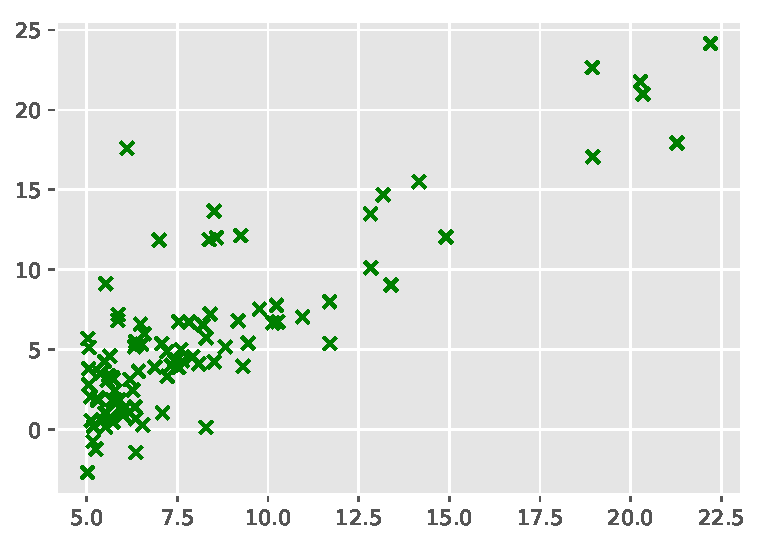
\includegraphics{assets/ex1_food_truck_profit.pdf}
\caption[Eine unskalierte PDF-Grafik]{Eine unskalierte PDF-Grafik mit langer Unterschrift
\autocite[vgl.][13]{Perez_PythonEcosystem_2011}}\label{ref_a_pdf_figure}
}
\end{figure}

These are the results. Ut accumsan tempus aliquam. Sed massa ex,
egestas non libero id, imperdiet scelerisque augue. Duis rutrum
ultrices arcu et ultricies. Proin vel elit eu magna mattis vehicula.
Sed ex erat, fringilla vel feugiat ut, fringilla non diam.

\begin{figure}[]
\hypertarget{ref_a_scaled_pdf_figure}{%
\centering
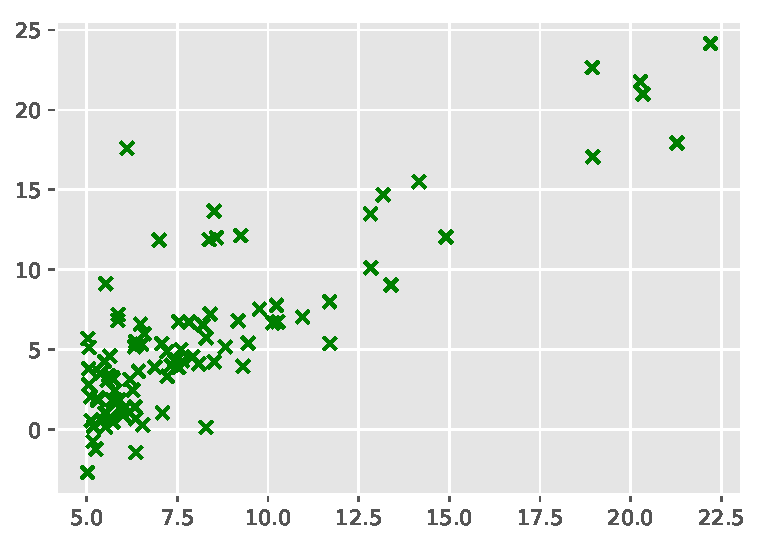
\includegraphics[width=0.70\textwidth]{assets/ex1_food_truck_profit.pdf}
\caption[Eine skalierte PDF-Grafik]{Eine skalierte PDF-Grafik mit langer Unterschrift
\autocite[vgl.][13]{Perez_PythonEcosystem_2011}}\label{ref_a_scaled_pdf_figure}
}
\end{figure}

This is the discussion. Duis ultrices tempor sem vitae convallis.
Pellentesque lobortis risus ac nisi varius bibendum. Phasellus
volutpat aliquam varius. Mauris vitae neque quis libero volutpat
finibus. Nunc diam metus, imperdiet vitae leo sed, varius posuere
orci.

\begin{figure}[]
\hypertarget{ref_a_pgf_figure}{%
\centering
%% Creator: Matplotlib, PGF backend
%%
%% To include the figure in your LaTeX document, write
%%   \input{<filename>.pgf}
%%
%% Make sure the required packages are loaded in your preamble
%%   \usepackage{pgf}
%%
%% Figures using additional raster images can only be included by \input if
%% they are in the same directory as the main LaTeX file. For loading figures
%% from other directories you can use the `import` package
%%   \usepackage{import}
%% and then include the figures with
%%   \import{<path to file>}{<filename>.pgf}
%%
%% Matplotlib used the following preamble
%%   \usepackage[utf8x]{inputenc}
%%   \usepackage[T1]{fontenc}
%%   \usepackage{cmbright}
%%   \usepackage{fontspec}
%%   \setmainfont{Times New Roman}
%%   \setsansfont{Verdana}
%%   \setmonofont{Courier New}
%%
\begingroup%
\makeatletter%
\begin{pgfpicture}%
\pgfpathrectangle{\pgfpointorigin}{\pgfqpoint{5.310640in}{3.844655in}}%
\pgfusepath{use as bounding box, clip}%
\begin{pgfscope}%
\pgfsetbuttcap%
\pgfsetmiterjoin%
\definecolor{currentfill}{rgb}{1.000000,1.000000,1.000000}%
\pgfsetfillcolor{currentfill}%
\pgfsetlinewidth{0.000000pt}%
\definecolor{currentstroke}{rgb}{1.000000,1.000000,1.000000}%
\pgfsetstrokecolor{currentstroke}%
\pgfsetdash{}{0pt}%
\pgfpathmoveto{\pgfqpoint{0.000000in}{0.000000in}}%
\pgfpathlineto{\pgfqpoint{5.310640in}{0.000000in}}%
\pgfpathlineto{\pgfqpoint{5.310640in}{3.844655in}}%
\pgfpathlineto{\pgfqpoint{0.000000in}{3.844655in}}%
\pgfpathclose%
\pgfusepath{fill}%
\end{pgfscope}%
\begin{pgfscope}%
\pgfsetbuttcap%
\pgfsetmiterjoin%
\definecolor{currentfill}{rgb}{0.898039,0.898039,0.898039}%
\pgfsetfillcolor{currentfill}%
\pgfsetlinewidth{0.000000pt}%
\definecolor{currentstroke}{rgb}{0.000000,0.000000,0.000000}%
\pgfsetstrokecolor{currentstroke}%
\pgfsetstrokeopacity{0.000000}%
\pgfsetdash{}{0pt}%
\pgfpathmoveto{\pgfqpoint{0.589529in}{0.546398in}}%
\pgfpathlineto{\pgfqpoint{5.162029in}{0.546398in}}%
\pgfpathlineto{\pgfqpoint{5.162029in}{3.696044in}}%
\pgfpathlineto{\pgfqpoint{0.589529in}{3.696044in}}%
\pgfpathclose%
\pgfusepath{fill}%
\end{pgfscope}%
\begin{pgfscope}%
\pgfpathrectangle{\pgfqpoint{0.589529in}{0.546398in}}{\pgfqpoint{4.572500in}{3.149646in}}%
\pgfusepath{clip}%
\pgfsetrectcap%
\pgfsetroundjoin%
\pgfsetlinewidth{0.803000pt}%
\definecolor{currentstroke}{rgb}{1.000000,1.000000,1.000000}%
\pgfsetstrokecolor{currentstroke}%
\pgfsetdash{}{0pt}%
\pgfpathmoveto{\pgfqpoint{0.793070in}{0.546398in}}%
\pgfpathlineto{\pgfqpoint{0.793070in}{3.696044in}}%
\pgfusepath{stroke}%
\end{pgfscope}%
\begin{pgfscope}%
\pgfsetbuttcap%
\pgfsetroundjoin%
\definecolor{currentfill}{rgb}{0.333333,0.333333,0.333333}%
\pgfsetfillcolor{currentfill}%
\pgfsetlinewidth{0.803000pt}%
\definecolor{currentstroke}{rgb}{0.333333,0.333333,0.333333}%
\pgfsetstrokecolor{currentstroke}%
\pgfsetdash{}{0pt}%
\pgfsys@defobject{currentmarker}{\pgfqpoint{0.000000in}{-0.048611in}}{\pgfqpoint{0.000000in}{0.000000in}}{%
\pgfpathmoveto{\pgfqpoint{0.000000in}{0.000000in}}%
\pgfpathlineto{\pgfqpoint{0.000000in}{-0.048611in}}%
\pgfusepath{stroke,fill}%
}%
\begin{pgfscope}%
\pgfsys@transformshift{0.793070in}{0.546398in}%
\pgfsys@useobject{currentmarker}{}%
\end{pgfscope}%
\end{pgfscope}%
\begin{pgfscope}%
\definecolor{textcolor}{rgb}{0.333333,0.333333,0.333333}%
\pgfsetstrokecolor{textcolor}%
\pgfsetfillcolor{textcolor}%
\pgftext[x=0.793070in,y=0.449175in,,top]{\color{textcolor}\sffamily\fontsize{10.000000}{12.000000}\selectfont 5.0}%
\end{pgfscope}%
\begin{pgfscope}%
\pgfpathrectangle{\pgfqpoint{0.589529in}{0.546398in}}{\pgfqpoint{4.572500in}{3.149646in}}%
\pgfusepath{clip}%
\pgfsetrectcap%
\pgfsetroundjoin%
\pgfsetlinewidth{0.803000pt}%
\definecolor{currentstroke}{rgb}{1.000000,1.000000,1.000000}%
\pgfsetstrokecolor{currentstroke}%
\pgfsetdash{}{0pt}%
\pgfpathmoveto{\pgfqpoint{1.397458in}{0.546398in}}%
\pgfpathlineto{\pgfqpoint{1.397458in}{3.696044in}}%
\pgfusepath{stroke}%
\end{pgfscope}%
\begin{pgfscope}%
\pgfsetbuttcap%
\pgfsetroundjoin%
\definecolor{currentfill}{rgb}{0.333333,0.333333,0.333333}%
\pgfsetfillcolor{currentfill}%
\pgfsetlinewidth{0.803000pt}%
\definecolor{currentstroke}{rgb}{0.333333,0.333333,0.333333}%
\pgfsetstrokecolor{currentstroke}%
\pgfsetdash{}{0pt}%
\pgfsys@defobject{currentmarker}{\pgfqpoint{0.000000in}{-0.048611in}}{\pgfqpoint{0.000000in}{0.000000in}}{%
\pgfpathmoveto{\pgfqpoint{0.000000in}{0.000000in}}%
\pgfpathlineto{\pgfqpoint{0.000000in}{-0.048611in}}%
\pgfusepath{stroke,fill}%
}%
\begin{pgfscope}%
\pgfsys@transformshift{1.397458in}{0.546398in}%
\pgfsys@useobject{currentmarker}{}%
\end{pgfscope}%
\end{pgfscope}%
\begin{pgfscope}%
\definecolor{textcolor}{rgb}{0.333333,0.333333,0.333333}%
\pgfsetstrokecolor{textcolor}%
\pgfsetfillcolor{textcolor}%
\pgftext[x=1.397458in,y=0.449175in,,top]{\color{textcolor}\sffamily\fontsize{10.000000}{12.000000}\selectfont 7.5}%
\end{pgfscope}%
\begin{pgfscope}%
\pgfpathrectangle{\pgfqpoint{0.589529in}{0.546398in}}{\pgfqpoint{4.572500in}{3.149646in}}%
\pgfusepath{clip}%
\pgfsetrectcap%
\pgfsetroundjoin%
\pgfsetlinewidth{0.803000pt}%
\definecolor{currentstroke}{rgb}{1.000000,1.000000,1.000000}%
\pgfsetstrokecolor{currentstroke}%
\pgfsetdash{}{0pt}%
\pgfpathmoveto{\pgfqpoint{2.001846in}{0.546398in}}%
\pgfpathlineto{\pgfqpoint{2.001846in}{3.696044in}}%
\pgfusepath{stroke}%
\end{pgfscope}%
\begin{pgfscope}%
\pgfsetbuttcap%
\pgfsetroundjoin%
\definecolor{currentfill}{rgb}{0.333333,0.333333,0.333333}%
\pgfsetfillcolor{currentfill}%
\pgfsetlinewidth{0.803000pt}%
\definecolor{currentstroke}{rgb}{0.333333,0.333333,0.333333}%
\pgfsetstrokecolor{currentstroke}%
\pgfsetdash{}{0pt}%
\pgfsys@defobject{currentmarker}{\pgfqpoint{0.000000in}{-0.048611in}}{\pgfqpoint{0.000000in}{0.000000in}}{%
\pgfpathmoveto{\pgfqpoint{0.000000in}{0.000000in}}%
\pgfpathlineto{\pgfqpoint{0.000000in}{-0.048611in}}%
\pgfusepath{stroke,fill}%
}%
\begin{pgfscope}%
\pgfsys@transformshift{2.001846in}{0.546398in}%
\pgfsys@useobject{currentmarker}{}%
\end{pgfscope}%
\end{pgfscope}%
\begin{pgfscope}%
\definecolor{textcolor}{rgb}{0.333333,0.333333,0.333333}%
\pgfsetstrokecolor{textcolor}%
\pgfsetfillcolor{textcolor}%
\pgftext[x=2.001846in,y=0.449175in,,top]{\color{textcolor}\sffamily\fontsize{10.000000}{12.000000}\selectfont 10.0}%
\end{pgfscope}%
\begin{pgfscope}%
\pgfpathrectangle{\pgfqpoint{0.589529in}{0.546398in}}{\pgfqpoint{4.572500in}{3.149646in}}%
\pgfusepath{clip}%
\pgfsetrectcap%
\pgfsetroundjoin%
\pgfsetlinewidth{0.803000pt}%
\definecolor{currentstroke}{rgb}{1.000000,1.000000,1.000000}%
\pgfsetstrokecolor{currentstroke}%
\pgfsetdash{}{0pt}%
\pgfpathmoveto{\pgfqpoint{2.606234in}{0.546398in}}%
\pgfpathlineto{\pgfqpoint{2.606234in}{3.696044in}}%
\pgfusepath{stroke}%
\end{pgfscope}%
\begin{pgfscope}%
\pgfsetbuttcap%
\pgfsetroundjoin%
\definecolor{currentfill}{rgb}{0.333333,0.333333,0.333333}%
\pgfsetfillcolor{currentfill}%
\pgfsetlinewidth{0.803000pt}%
\definecolor{currentstroke}{rgb}{0.333333,0.333333,0.333333}%
\pgfsetstrokecolor{currentstroke}%
\pgfsetdash{}{0pt}%
\pgfsys@defobject{currentmarker}{\pgfqpoint{0.000000in}{-0.048611in}}{\pgfqpoint{0.000000in}{0.000000in}}{%
\pgfpathmoveto{\pgfqpoint{0.000000in}{0.000000in}}%
\pgfpathlineto{\pgfqpoint{0.000000in}{-0.048611in}}%
\pgfusepath{stroke,fill}%
}%
\begin{pgfscope}%
\pgfsys@transformshift{2.606234in}{0.546398in}%
\pgfsys@useobject{currentmarker}{}%
\end{pgfscope}%
\end{pgfscope}%
\begin{pgfscope}%
\definecolor{textcolor}{rgb}{0.333333,0.333333,0.333333}%
\pgfsetstrokecolor{textcolor}%
\pgfsetfillcolor{textcolor}%
\pgftext[x=2.606234in,y=0.449175in,,top]{\color{textcolor}\sffamily\fontsize{10.000000}{12.000000}\selectfont 12.5}%
\end{pgfscope}%
\begin{pgfscope}%
\pgfpathrectangle{\pgfqpoint{0.589529in}{0.546398in}}{\pgfqpoint{4.572500in}{3.149646in}}%
\pgfusepath{clip}%
\pgfsetrectcap%
\pgfsetroundjoin%
\pgfsetlinewidth{0.803000pt}%
\definecolor{currentstroke}{rgb}{1.000000,1.000000,1.000000}%
\pgfsetstrokecolor{currentstroke}%
\pgfsetdash{}{0pt}%
\pgfpathmoveto{\pgfqpoint{3.210622in}{0.546398in}}%
\pgfpathlineto{\pgfqpoint{3.210622in}{3.696044in}}%
\pgfusepath{stroke}%
\end{pgfscope}%
\begin{pgfscope}%
\pgfsetbuttcap%
\pgfsetroundjoin%
\definecolor{currentfill}{rgb}{0.333333,0.333333,0.333333}%
\pgfsetfillcolor{currentfill}%
\pgfsetlinewidth{0.803000pt}%
\definecolor{currentstroke}{rgb}{0.333333,0.333333,0.333333}%
\pgfsetstrokecolor{currentstroke}%
\pgfsetdash{}{0pt}%
\pgfsys@defobject{currentmarker}{\pgfqpoint{0.000000in}{-0.048611in}}{\pgfqpoint{0.000000in}{0.000000in}}{%
\pgfpathmoveto{\pgfqpoint{0.000000in}{0.000000in}}%
\pgfpathlineto{\pgfqpoint{0.000000in}{-0.048611in}}%
\pgfusepath{stroke,fill}%
}%
\begin{pgfscope}%
\pgfsys@transformshift{3.210622in}{0.546398in}%
\pgfsys@useobject{currentmarker}{}%
\end{pgfscope}%
\end{pgfscope}%
\begin{pgfscope}%
\definecolor{textcolor}{rgb}{0.333333,0.333333,0.333333}%
\pgfsetstrokecolor{textcolor}%
\pgfsetfillcolor{textcolor}%
\pgftext[x=3.210622in,y=0.449175in,,top]{\color{textcolor}\sffamily\fontsize{10.000000}{12.000000}\selectfont 15.0}%
\end{pgfscope}%
\begin{pgfscope}%
\pgfpathrectangle{\pgfqpoint{0.589529in}{0.546398in}}{\pgfqpoint{4.572500in}{3.149646in}}%
\pgfusepath{clip}%
\pgfsetrectcap%
\pgfsetroundjoin%
\pgfsetlinewidth{0.803000pt}%
\definecolor{currentstroke}{rgb}{1.000000,1.000000,1.000000}%
\pgfsetstrokecolor{currentstroke}%
\pgfsetdash{}{0pt}%
\pgfpathmoveto{\pgfqpoint{3.815010in}{0.546398in}}%
\pgfpathlineto{\pgfqpoint{3.815010in}{3.696044in}}%
\pgfusepath{stroke}%
\end{pgfscope}%
\begin{pgfscope}%
\pgfsetbuttcap%
\pgfsetroundjoin%
\definecolor{currentfill}{rgb}{0.333333,0.333333,0.333333}%
\pgfsetfillcolor{currentfill}%
\pgfsetlinewidth{0.803000pt}%
\definecolor{currentstroke}{rgb}{0.333333,0.333333,0.333333}%
\pgfsetstrokecolor{currentstroke}%
\pgfsetdash{}{0pt}%
\pgfsys@defobject{currentmarker}{\pgfqpoint{0.000000in}{-0.048611in}}{\pgfqpoint{0.000000in}{0.000000in}}{%
\pgfpathmoveto{\pgfqpoint{0.000000in}{0.000000in}}%
\pgfpathlineto{\pgfqpoint{0.000000in}{-0.048611in}}%
\pgfusepath{stroke,fill}%
}%
\begin{pgfscope}%
\pgfsys@transformshift{3.815010in}{0.546398in}%
\pgfsys@useobject{currentmarker}{}%
\end{pgfscope}%
\end{pgfscope}%
\begin{pgfscope}%
\definecolor{textcolor}{rgb}{0.333333,0.333333,0.333333}%
\pgfsetstrokecolor{textcolor}%
\pgfsetfillcolor{textcolor}%
\pgftext[x=3.815010in,y=0.449175in,,top]{\color{textcolor}\sffamily\fontsize{10.000000}{12.000000}\selectfont 17.5}%
\end{pgfscope}%
\begin{pgfscope}%
\pgfpathrectangle{\pgfqpoint{0.589529in}{0.546398in}}{\pgfqpoint{4.572500in}{3.149646in}}%
\pgfusepath{clip}%
\pgfsetrectcap%
\pgfsetroundjoin%
\pgfsetlinewidth{0.803000pt}%
\definecolor{currentstroke}{rgb}{1.000000,1.000000,1.000000}%
\pgfsetstrokecolor{currentstroke}%
\pgfsetdash{}{0pt}%
\pgfpathmoveto{\pgfqpoint{4.419398in}{0.546398in}}%
\pgfpathlineto{\pgfqpoint{4.419398in}{3.696044in}}%
\pgfusepath{stroke}%
\end{pgfscope}%
\begin{pgfscope}%
\pgfsetbuttcap%
\pgfsetroundjoin%
\definecolor{currentfill}{rgb}{0.333333,0.333333,0.333333}%
\pgfsetfillcolor{currentfill}%
\pgfsetlinewidth{0.803000pt}%
\definecolor{currentstroke}{rgb}{0.333333,0.333333,0.333333}%
\pgfsetstrokecolor{currentstroke}%
\pgfsetdash{}{0pt}%
\pgfsys@defobject{currentmarker}{\pgfqpoint{0.000000in}{-0.048611in}}{\pgfqpoint{0.000000in}{0.000000in}}{%
\pgfpathmoveto{\pgfqpoint{0.000000in}{0.000000in}}%
\pgfpathlineto{\pgfqpoint{0.000000in}{-0.048611in}}%
\pgfusepath{stroke,fill}%
}%
\begin{pgfscope}%
\pgfsys@transformshift{4.419398in}{0.546398in}%
\pgfsys@useobject{currentmarker}{}%
\end{pgfscope}%
\end{pgfscope}%
\begin{pgfscope}%
\definecolor{textcolor}{rgb}{0.333333,0.333333,0.333333}%
\pgfsetstrokecolor{textcolor}%
\pgfsetfillcolor{textcolor}%
\pgftext[x=4.419398in,y=0.449175in,,top]{\color{textcolor}\sffamily\fontsize{10.000000}{12.000000}\selectfont 20.0}%
\end{pgfscope}%
\begin{pgfscope}%
\pgfpathrectangle{\pgfqpoint{0.589529in}{0.546398in}}{\pgfqpoint{4.572500in}{3.149646in}}%
\pgfusepath{clip}%
\pgfsetrectcap%
\pgfsetroundjoin%
\pgfsetlinewidth{0.803000pt}%
\definecolor{currentstroke}{rgb}{1.000000,1.000000,1.000000}%
\pgfsetstrokecolor{currentstroke}%
\pgfsetdash{}{0pt}%
\pgfpathmoveto{\pgfqpoint{5.023786in}{0.546398in}}%
\pgfpathlineto{\pgfqpoint{5.023786in}{3.696044in}}%
\pgfusepath{stroke}%
\end{pgfscope}%
\begin{pgfscope}%
\pgfsetbuttcap%
\pgfsetroundjoin%
\definecolor{currentfill}{rgb}{0.333333,0.333333,0.333333}%
\pgfsetfillcolor{currentfill}%
\pgfsetlinewidth{0.803000pt}%
\definecolor{currentstroke}{rgb}{0.333333,0.333333,0.333333}%
\pgfsetstrokecolor{currentstroke}%
\pgfsetdash{}{0pt}%
\pgfsys@defobject{currentmarker}{\pgfqpoint{0.000000in}{-0.048611in}}{\pgfqpoint{0.000000in}{0.000000in}}{%
\pgfpathmoveto{\pgfqpoint{0.000000in}{0.000000in}}%
\pgfpathlineto{\pgfqpoint{0.000000in}{-0.048611in}}%
\pgfusepath{stroke,fill}%
}%
\begin{pgfscope}%
\pgfsys@transformshift{5.023786in}{0.546398in}%
\pgfsys@useobject{currentmarker}{}%
\end{pgfscope}%
\end{pgfscope}%
\begin{pgfscope}%
\definecolor{textcolor}{rgb}{0.333333,0.333333,0.333333}%
\pgfsetstrokecolor{textcolor}%
\pgfsetfillcolor{textcolor}%
\pgftext[x=5.023786in,y=0.449175in,,top]{\color{textcolor}\sffamily\fontsize{10.000000}{12.000000}\selectfont 22.5}%
\end{pgfscope}%
\begin{pgfscope}%
\definecolor{textcolor}{rgb}{0.333333,0.333333,0.333333}%
\pgfsetstrokecolor{textcolor}%
\pgfsetfillcolor{textcolor}%
\pgftext[x=2.875779in,y=0.260156in,,top]{\color{textcolor}\sffamily\fontsize{12.000000}{14.400000}\selectfont Population in 10000s}%
\end{pgfscope}%
\begin{pgfscope}%
\pgfpathrectangle{\pgfqpoint{0.589529in}{0.546398in}}{\pgfqpoint{4.572500in}{3.149646in}}%
\pgfusepath{clip}%
\pgfsetrectcap%
\pgfsetroundjoin%
\pgfsetlinewidth{0.803000pt}%
\definecolor{currentstroke}{rgb}{1.000000,1.000000,1.000000}%
\pgfsetstrokecolor{currentstroke}%
\pgfsetdash{}{0pt}%
\pgfpathmoveto{\pgfqpoint{0.589529in}{0.976803in}}%
\pgfpathlineto{\pgfqpoint{5.162029in}{0.976803in}}%
\pgfusepath{stroke}%
\end{pgfscope}%
\begin{pgfscope}%
\pgfsetbuttcap%
\pgfsetroundjoin%
\definecolor{currentfill}{rgb}{0.333333,0.333333,0.333333}%
\pgfsetfillcolor{currentfill}%
\pgfsetlinewidth{0.803000pt}%
\definecolor{currentstroke}{rgb}{0.333333,0.333333,0.333333}%
\pgfsetstrokecolor{currentstroke}%
\pgfsetdash{}{0pt}%
\pgfsys@defobject{currentmarker}{\pgfqpoint{-0.048611in}{0.000000in}}{\pgfqpoint{0.000000in}{0.000000in}}{%
\pgfpathmoveto{\pgfqpoint{0.000000in}{0.000000in}}%
\pgfpathlineto{\pgfqpoint{-0.048611in}{0.000000in}}%
\pgfusepath{stroke,fill}%
}%
\begin{pgfscope}%
\pgfsys@transformshift{0.589529in}{0.976803in}%
\pgfsys@useobject{currentmarker}{}%
\end{pgfscope}%
\end{pgfscope}%
\begin{pgfscope}%
\definecolor{textcolor}{rgb}{0.333333,0.333333,0.333333}%
\pgfsetstrokecolor{textcolor}%
\pgfsetfillcolor{textcolor}%
\pgftext[x=0.404009in,y=0.924041in,left,base]{\color{textcolor}\sffamily\fontsize{10.000000}{12.000000}\selectfont 0}%
\end{pgfscope}%
\begin{pgfscope}%
\pgfpathrectangle{\pgfqpoint{0.589529in}{0.546398in}}{\pgfqpoint{4.572500in}{3.149646in}}%
\pgfusepath{clip}%
\pgfsetrectcap%
\pgfsetroundjoin%
\pgfsetlinewidth{0.803000pt}%
\definecolor{currentstroke}{rgb}{1.000000,1.000000,1.000000}%
\pgfsetstrokecolor{currentstroke}%
\pgfsetdash{}{0pt}%
\pgfpathmoveto{\pgfqpoint{0.589529in}{1.509926in}}%
\pgfpathlineto{\pgfqpoint{5.162029in}{1.509926in}}%
\pgfusepath{stroke}%
\end{pgfscope}%
\begin{pgfscope}%
\pgfsetbuttcap%
\pgfsetroundjoin%
\definecolor{currentfill}{rgb}{0.333333,0.333333,0.333333}%
\pgfsetfillcolor{currentfill}%
\pgfsetlinewidth{0.803000pt}%
\definecolor{currentstroke}{rgb}{0.333333,0.333333,0.333333}%
\pgfsetstrokecolor{currentstroke}%
\pgfsetdash{}{0pt}%
\pgfsys@defobject{currentmarker}{\pgfqpoint{-0.048611in}{0.000000in}}{\pgfqpoint{0.000000in}{0.000000in}}{%
\pgfpathmoveto{\pgfqpoint{0.000000in}{0.000000in}}%
\pgfpathlineto{\pgfqpoint{-0.048611in}{0.000000in}}%
\pgfusepath{stroke,fill}%
}%
\begin{pgfscope}%
\pgfsys@transformshift{0.589529in}{1.509926in}%
\pgfsys@useobject{currentmarker}{}%
\end{pgfscope}%
\end{pgfscope}%
\begin{pgfscope}%
\definecolor{textcolor}{rgb}{0.333333,0.333333,0.333333}%
\pgfsetstrokecolor{textcolor}%
\pgfsetfillcolor{textcolor}%
\pgftext[x=0.404009in,y=1.457164in,left,base]{\color{textcolor}\sffamily\fontsize{10.000000}{12.000000}\selectfont 5}%
\end{pgfscope}%
\begin{pgfscope}%
\pgfpathrectangle{\pgfqpoint{0.589529in}{0.546398in}}{\pgfqpoint{4.572500in}{3.149646in}}%
\pgfusepath{clip}%
\pgfsetrectcap%
\pgfsetroundjoin%
\pgfsetlinewidth{0.803000pt}%
\definecolor{currentstroke}{rgb}{1.000000,1.000000,1.000000}%
\pgfsetstrokecolor{currentstroke}%
\pgfsetdash{}{0pt}%
\pgfpathmoveto{\pgfqpoint{0.589529in}{2.043049in}}%
\pgfpathlineto{\pgfqpoint{5.162029in}{2.043049in}}%
\pgfusepath{stroke}%
\end{pgfscope}%
\begin{pgfscope}%
\pgfsetbuttcap%
\pgfsetroundjoin%
\definecolor{currentfill}{rgb}{0.333333,0.333333,0.333333}%
\pgfsetfillcolor{currentfill}%
\pgfsetlinewidth{0.803000pt}%
\definecolor{currentstroke}{rgb}{0.333333,0.333333,0.333333}%
\pgfsetstrokecolor{currentstroke}%
\pgfsetdash{}{0pt}%
\pgfsys@defobject{currentmarker}{\pgfqpoint{-0.048611in}{0.000000in}}{\pgfqpoint{0.000000in}{0.000000in}}{%
\pgfpathmoveto{\pgfqpoint{0.000000in}{0.000000in}}%
\pgfpathlineto{\pgfqpoint{-0.048611in}{0.000000in}}%
\pgfusepath{stroke,fill}%
}%
\begin{pgfscope}%
\pgfsys@transformshift{0.589529in}{2.043049in}%
\pgfsys@useobject{currentmarker}{}%
\end{pgfscope}%
\end{pgfscope}%
\begin{pgfscope}%
\definecolor{textcolor}{rgb}{0.333333,0.333333,0.333333}%
\pgfsetstrokecolor{textcolor}%
\pgfsetfillcolor{textcolor}%
\pgftext[x=0.315712in,y=1.990287in,left,base]{\color{textcolor}\sffamily\fontsize{10.000000}{12.000000}\selectfont 10}%
\end{pgfscope}%
\begin{pgfscope}%
\pgfpathrectangle{\pgfqpoint{0.589529in}{0.546398in}}{\pgfqpoint{4.572500in}{3.149646in}}%
\pgfusepath{clip}%
\pgfsetrectcap%
\pgfsetroundjoin%
\pgfsetlinewidth{0.803000pt}%
\definecolor{currentstroke}{rgb}{1.000000,1.000000,1.000000}%
\pgfsetstrokecolor{currentstroke}%
\pgfsetdash{}{0pt}%
\pgfpathmoveto{\pgfqpoint{0.589529in}{2.576172in}}%
\pgfpathlineto{\pgfqpoint{5.162029in}{2.576172in}}%
\pgfusepath{stroke}%
\end{pgfscope}%
\begin{pgfscope}%
\pgfsetbuttcap%
\pgfsetroundjoin%
\definecolor{currentfill}{rgb}{0.333333,0.333333,0.333333}%
\pgfsetfillcolor{currentfill}%
\pgfsetlinewidth{0.803000pt}%
\definecolor{currentstroke}{rgb}{0.333333,0.333333,0.333333}%
\pgfsetstrokecolor{currentstroke}%
\pgfsetdash{}{0pt}%
\pgfsys@defobject{currentmarker}{\pgfqpoint{-0.048611in}{0.000000in}}{\pgfqpoint{0.000000in}{0.000000in}}{%
\pgfpathmoveto{\pgfqpoint{0.000000in}{0.000000in}}%
\pgfpathlineto{\pgfqpoint{-0.048611in}{0.000000in}}%
\pgfusepath{stroke,fill}%
}%
\begin{pgfscope}%
\pgfsys@transformshift{0.589529in}{2.576172in}%
\pgfsys@useobject{currentmarker}{}%
\end{pgfscope}%
\end{pgfscope}%
\begin{pgfscope}%
\definecolor{textcolor}{rgb}{0.333333,0.333333,0.333333}%
\pgfsetstrokecolor{textcolor}%
\pgfsetfillcolor{textcolor}%
\pgftext[x=0.315712in,y=2.523411in,left,base]{\color{textcolor}\sffamily\fontsize{10.000000}{12.000000}\selectfont 15}%
\end{pgfscope}%
\begin{pgfscope}%
\pgfpathrectangle{\pgfqpoint{0.589529in}{0.546398in}}{\pgfqpoint{4.572500in}{3.149646in}}%
\pgfusepath{clip}%
\pgfsetrectcap%
\pgfsetroundjoin%
\pgfsetlinewidth{0.803000pt}%
\definecolor{currentstroke}{rgb}{1.000000,1.000000,1.000000}%
\pgfsetstrokecolor{currentstroke}%
\pgfsetdash{}{0pt}%
\pgfpathmoveto{\pgfqpoint{0.589529in}{3.109295in}}%
\pgfpathlineto{\pgfqpoint{5.162029in}{3.109295in}}%
\pgfusepath{stroke}%
\end{pgfscope}%
\begin{pgfscope}%
\pgfsetbuttcap%
\pgfsetroundjoin%
\definecolor{currentfill}{rgb}{0.333333,0.333333,0.333333}%
\pgfsetfillcolor{currentfill}%
\pgfsetlinewidth{0.803000pt}%
\definecolor{currentstroke}{rgb}{0.333333,0.333333,0.333333}%
\pgfsetstrokecolor{currentstroke}%
\pgfsetdash{}{0pt}%
\pgfsys@defobject{currentmarker}{\pgfqpoint{-0.048611in}{0.000000in}}{\pgfqpoint{0.000000in}{0.000000in}}{%
\pgfpathmoveto{\pgfqpoint{0.000000in}{0.000000in}}%
\pgfpathlineto{\pgfqpoint{-0.048611in}{0.000000in}}%
\pgfusepath{stroke,fill}%
}%
\begin{pgfscope}%
\pgfsys@transformshift{0.589529in}{3.109295in}%
\pgfsys@useobject{currentmarker}{}%
\end{pgfscope}%
\end{pgfscope}%
\begin{pgfscope}%
\definecolor{textcolor}{rgb}{0.333333,0.333333,0.333333}%
\pgfsetstrokecolor{textcolor}%
\pgfsetfillcolor{textcolor}%
\pgftext[x=0.315712in,y=3.056534in,left,base]{\color{textcolor}\sffamily\fontsize{10.000000}{12.000000}\selectfont 20}%
\end{pgfscope}%
\begin{pgfscope}%
\pgfpathrectangle{\pgfqpoint{0.589529in}{0.546398in}}{\pgfqpoint{4.572500in}{3.149646in}}%
\pgfusepath{clip}%
\pgfsetrectcap%
\pgfsetroundjoin%
\pgfsetlinewidth{0.803000pt}%
\definecolor{currentstroke}{rgb}{1.000000,1.000000,1.000000}%
\pgfsetstrokecolor{currentstroke}%
\pgfsetdash{}{0pt}%
\pgfpathmoveto{\pgfqpoint{0.589529in}{3.642419in}}%
\pgfpathlineto{\pgfqpoint{5.162029in}{3.642419in}}%
\pgfusepath{stroke}%
\end{pgfscope}%
\begin{pgfscope}%
\pgfsetbuttcap%
\pgfsetroundjoin%
\definecolor{currentfill}{rgb}{0.333333,0.333333,0.333333}%
\pgfsetfillcolor{currentfill}%
\pgfsetlinewidth{0.803000pt}%
\definecolor{currentstroke}{rgb}{0.333333,0.333333,0.333333}%
\pgfsetstrokecolor{currentstroke}%
\pgfsetdash{}{0pt}%
\pgfsys@defobject{currentmarker}{\pgfqpoint{-0.048611in}{0.000000in}}{\pgfqpoint{0.000000in}{0.000000in}}{%
\pgfpathmoveto{\pgfqpoint{0.000000in}{0.000000in}}%
\pgfpathlineto{\pgfqpoint{-0.048611in}{0.000000in}}%
\pgfusepath{stroke,fill}%
}%
\begin{pgfscope}%
\pgfsys@transformshift{0.589529in}{3.642419in}%
\pgfsys@useobject{currentmarker}{}%
\end{pgfscope}%
\end{pgfscope}%
\begin{pgfscope}%
\definecolor{textcolor}{rgb}{0.333333,0.333333,0.333333}%
\pgfsetstrokecolor{textcolor}%
\pgfsetfillcolor{textcolor}%
\pgftext[x=0.315712in,y=3.589657in,left,base]{\color{textcolor}\sffamily\fontsize{10.000000}{12.000000}\selectfont 25}%
\end{pgfscope}%
\begin{pgfscope}%
\definecolor{textcolor}{rgb}{0.333333,0.333333,0.333333}%
\pgfsetstrokecolor{textcolor}%
\pgfsetfillcolor{textcolor}%
\pgftext[x=0.260156in,y=2.121221in,,bottom,rotate=90.000000]{\color{textcolor}\sffamily\fontsize{12.000000}{14.400000}\selectfont Profit in \(\displaystyle 10000s\)}%
\end{pgfscope}%
\begin{pgfscope}%
\pgfpathrectangle{\pgfqpoint{0.589529in}{0.546398in}}{\pgfqpoint{4.572500in}{3.149646in}}%
\pgfusepath{clip}%
\pgfsetbuttcap%
\pgfsetroundjoin%
\definecolor{currentfill}{rgb}{0.000000,0.500000,0.000000}%
\pgfsetfillcolor{currentfill}%
\pgfsetlinewidth{1.505625pt}%
\definecolor{currentstroke}{rgb}{0.000000,0.500000,0.000000}%
\pgfsetstrokecolor{currentstroke}%
\pgfsetdash{}{0pt}%
\pgfpathmoveto{\pgfqpoint{1.019776in}{2.810877in}}%
\pgfpathlineto{\pgfqpoint{1.103109in}{2.894210in}}%
\pgfpathmoveto{\pgfqpoint{1.019776in}{2.894210in}}%
\pgfpathlineto{\pgfqpoint{1.103109in}{2.810877in}}%
\pgfusepath{stroke,fill}%
\end{pgfscope}%
\begin{pgfscope}%
\pgfpathrectangle{\pgfqpoint{0.589529in}{0.546398in}}{\pgfqpoint{4.572500in}{3.149646in}}%
\pgfusepath{clip}%
\pgfsetbuttcap%
\pgfsetroundjoin%
\definecolor{currentfill}{rgb}{0.000000,0.500000,0.000000}%
\pgfsetfillcolor{currentfill}%
\pgfsetlinewidth{1.505625pt}%
\definecolor{currentstroke}{rgb}{0.000000,0.500000,0.000000}%
\pgfsetstrokecolor{currentstroke}%
\pgfsetdash{}{0pt}%
\pgfpathmoveto{\pgfqpoint{0.878977in}{1.908640in}}%
\pgfpathlineto{\pgfqpoint{0.962311in}{1.991974in}}%
\pgfpathmoveto{\pgfqpoint{0.878977in}{1.991974in}}%
\pgfpathlineto{\pgfqpoint{0.962311in}{1.908640in}}%
\pgfusepath{stroke,fill}%
\end{pgfscope}%
\begin{pgfscope}%
\pgfpathrectangle{\pgfqpoint{0.589529in}{0.546398in}}{\pgfqpoint{4.572500in}{3.149646in}}%
\pgfusepath{clip}%
\pgfsetbuttcap%
\pgfsetroundjoin%
\definecolor{currentfill}{rgb}{0.000000,0.500000,0.000000}%
\pgfsetfillcolor{currentfill}%
\pgfsetlinewidth{1.505625pt}%
\definecolor{currentstroke}{rgb}{0.000000,0.500000,0.000000}%
\pgfsetstrokecolor{currentstroke}%
\pgfsetdash{}{0pt}%
\pgfpathmoveto{\pgfqpoint{1.602043in}{2.391842in}}%
\pgfpathlineto{\pgfqpoint{1.685376in}{2.475175in}}%
\pgfpathmoveto{\pgfqpoint{1.602043in}{2.475175in}}%
\pgfpathlineto{\pgfqpoint{1.685376in}{2.391842in}}%
\pgfusepath{stroke,fill}%
\end{pgfscope}%
\begin{pgfscope}%
\pgfpathrectangle{\pgfqpoint{0.589529in}{0.546398in}}{\pgfqpoint{4.572500in}{3.149646in}}%
\pgfusepath{clip}%
\pgfsetbuttcap%
\pgfsetroundjoin%
\definecolor{currentfill}{rgb}{0.000000,0.500000,0.000000}%
\pgfsetfillcolor{currentfill}%
\pgfsetlinewidth{1.505625pt}%
\definecolor{currentstroke}{rgb}{0.000000,0.500000,0.000000}%
\pgfsetstrokecolor{currentstroke}%
\pgfsetdash{}{0pt}%
\pgfpathmoveto{\pgfqpoint{1.235687in}{2.199064in}}%
\pgfpathlineto{\pgfqpoint{1.319020in}{2.282398in}}%
\pgfpathmoveto{\pgfqpoint{1.235687in}{2.282398in}}%
\pgfpathlineto{\pgfqpoint{1.319020in}{2.199064in}}%
\pgfusepath{stroke,fill}%
\end{pgfscope}%
\begin{pgfscope}%
\pgfpathrectangle{\pgfqpoint{0.589529in}{0.546398in}}{\pgfqpoint{4.572500in}{3.149646in}}%
\pgfusepath{clip}%
\pgfsetbuttcap%
\pgfsetroundjoin%
\definecolor{currentfill}{rgb}{0.000000,0.500000,0.000000}%
\pgfsetfillcolor{currentfill}%
\pgfsetlinewidth{1.505625pt}%
\definecolor{currentstroke}{rgb}{0.000000,0.500000,0.000000}%
\pgfsetstrokecolor{currentstroke}%
\pgfsetdash{}{0pt}%
\pgfpathmoveto{\pgfqpoint{0.959264in}{1.662668in}}%
\pgfpathlineto{\pgfqpoint{1.042598in}{1.746001in}}%
\pgfpathmoveto{\pgfqpoint{0.959264in}{1.746001in}}%
\pgfpathlineto{\pgfqpoint{1.042598in}{1.662668in}}%
\pgfusepath{stroke,fill}%
\end{pgfscope}%
\begin{pgfscope}%
\pgfpathrectangle{\pgfqpoint{0.589529in}{0.546398in}}{\pgfqpoint{4.572500in}{3.149646in}}%
\pgfusepath{clip}%
\pgfsetbuttcap%
\pgfsetroundjoin%
\definecolor{currentfill}{rgb}{0.000000,0.500000,0.000000}%
\pgfsetfillcolor{currentfill}%
\pgfsetlinewidth{1.505625pt}%
\definecolor{currentstroke}{rgb}{0.000000,0.500000,0.000000}%
\pgfsetstrokecolor{currentstroke}%
\pgfsetdash{}{0pt}%
\pgfpathmoveto{\pgfqpoint{1.569237in}{2.202476in}}%
\pgfpathlineto{\pgfqpoint{1.652570in}{2.285810in}}%
\pgfpathmoveto{\pgfqpoint{1.569237in}{2.285810in}}%
\pgfpathlineto{\pgfqpoint{1.652570in}{2.202476in}}%
\pgfusepath{stroke,fill}%
\end{pgfscope}%
\begin{pgfscope}%
\pgfpathrectangle{\pgfqpoint{0.589529in}{0.546398in}}{\pgfqpoint{4.572500in}{3.149646in}}%
\pgfusepath{clip}%
\pgfsetbuttcap%
\pgfsetroundjoin%
\definecolor{currentfill}{rgb}{0.000000,0.500000,0.000000}%
\pgfsetfillcolor{currentfill}%
\pgfsetlinewidth{1.505625pt}%
\definecolor{currentstroke}{rgb}{0.000000,0.500000,0.000000}%
\pgfsetstrokecolor{currentstroke}%
\pgfsetdash{}{0pt}%
\pgfpathmoveto{\pgfqpoint{1.350086in}{1.398772in}}%
\pgfpathlineto{\pgfqpoint{1.433419in}{1.482105in}}%
\pgfpathmoveto{\pgfqpoint{1.350086in}{1.482105in}}%
\pgfpathlineto{\pgfqpoint{1.433419in}{1.398772in}}%
\pgfusepath{stroke,fill}%
\end{pgfscope}%
\begin{pgfscope}%
\pgfpathrectangle{\pgfqpoint{0.589529in}{0.546398in}}{\pgfqpoint{4.572500in}{3.149646in}}%
\pgfusepath{clip}%
\pgfsetbuttcap%
\pgfsetroundjoin%
\definecolor{currentfill}{rgb}{0.000000,0.500000,0.000000}%
\pgfsetfillcolor{currentfill}%
\pgfsetlinewidth{1.505625pt}%
\definecolor{currentstroke}{rgb}{0.000000,0.500000,0.000000}%
\pgfsetstrokecolor{currentstroke}%
\pgfsetdash{}{0pt}%
\pgfpathmoveto{\pgfqpoint{1.616427in}{2.214632in}}%
\pgfpathlineto{\pgfqpoint{1.699761in}{2.297965in}}%
\pgfpathmoveto{\pgfqpoint{1.616427in}{2.297965in}}%
\pgfpathlineto{\pgfqpoint{1.699761in}{2.214632in}}%
\pgfusepath{stroke,fill}%
\end{pgfscope}%
\begin{pgfscope}%
\pgfpathrectangle{\pgfqpoint{0.589529in}{0.546398in}}{\pgfqpoint{4.572500in}{3.149646in}}%
\pgfusepath{clip}%
\pgfsetbuttcap%
\pgfsetroundjoin%
\definecolor{currentfill}{rgb}{0.000000,0.500000,0.000000}%
\pgfsetfillcolor{currentfill}%
\pgfsetlinewidth{1.505625pt}%
\definecolor{currentstroke}{rgb}{0.000000,0.500000,0.000000}%
\pgfsetstrokecolor{currentstroke}%
\pgfsetdash{}{0pt}%
\pgfpathmoveto{\pgfqpoint{1.110700in}{1.638720in}}%
\pgfpathlineto{\pgfqpoint{1.194033in}{1.722053in}}%
\pgfpathmoveto{\pgfqpoint{1.110700in}{1.722053in}}%
\pgfpathlineto{\pgfqpoint{1.194033in}{1.638720in}}%
\pgfusepath{stroke,fill}%
\end{pgfscope}%
\begin{pgfscope}%
\pgfpathrectangle{\pgfqpoint{0.589529in}{0.546398in}}{\pgfqpoint{4.572500in}{3.149646in}}%
\pgfusepath{clip}%
\pgfsetbuttcap%
\pgfsetroundjoin%
\definecolor{currentfill}{rgb}{0.000000,0.500000,0.000000}%
\pgfsetfillcolor{currentfill}%
\pgfsetlinewidth{1.505625pt}%
\definecolor{currentstroke}{rgb}{0.000000,0.500000,0.000000}%
\pgfsetstrokecolor{currentstroke}%
\pgfsetdash{}{0pt}%
\pgfpathmoveto{\pgfqpoint{0.764603in}{1.342080in}}%
\pgfpathlineto{\pgfqpoint{0.847936in}{1.425413in}}%
\pgfpathmoveto{\pgfqpoint{0.764603in}{1.425413in}}%
\pgfpathlineto{\pgfqpoint{0.847936in}{1.342080in}}%
\pgfusepath{stroke,fill}%
\end{pgfscope}%
\begin{pgfscope}%
\pgfpathrectangle{\pgfqpoint{0.589529in}{0.546398in}}{\pgfqpoint{4.572500in}{3.149646in}}%
\pgfusepath{clip}%
\pgfsetbuttcap%
\pgfsetroundjoin%
\definecolor{currentfill}{rgb}{0.000000,0.500000,0.000000}%
\pgfsetfillcolor{currentfill}%
\pgfsetlinewidth{1.505625pt}%
\definecolor{currentstroke}{rgb}{0.000000,0.500000,0.000000}%
\pgfsetstrokecolor{currentstroke}%
\pgfsetdash{}{0pt}%
\pgfpathmoveto{\pgfqpoint{0.923218in}{1.281901in}}%
\pgfpathlineto{\pgfqpoint{1.006552in}{1.365234in}}%
\pgfpathmoveto{\pgfqpoint{0.923218in}{1.365234in}}%
\pgfpathlineto{\pgfqpoint{1.006552in}{1.281901in}}%
\pgfusepath{stroke,fill}%
\end{pgfscope}%
\begin{pgfscope}%
\pgfpathrectangle{\pgfqpoint{0.589529in}{0.546398in}}{\pgfqpoint{4.572500in}{3.149646in}}%
\pgfusepath{clip}%
\pgfsetbuttcap%
\pgfsetroundjoin%
\definecolor{currentfill}{rgb}{0.000000,0.500000,0.000000}%
\pgfsetfillcolor{currentfill}%
\pgfsetlinewidth{1.505625pt}%
\definecolor{currentstroke}{rgb}{0.000000,0.500000,0.000000}%
\pgfsetstrokecolor{currentstroke}%
\pgfsetdash{}{0pt}%
\pgfpathmoveto{\pgfqpoint{2.966848in}{2.588351in}}%
\pgfpathlineto{\pgfqpoint{3.050181in}{2.671684in}}%
\pgfpathmoveto{\pgfqpoint{2.966848in}{2.671684in}}%
\pgfpathlineto{\pgfqpoint{3.050181in}{2.588351in}}%
\pgfusepath{stroke,fill}%
\end{pgfscope}%
\begin{pgfscope}%
\pgfpathrectangle{\pgfqpoint{0.589529in}{0.546398in}}{\pgfqpoint{4.572500in}{3.149646in}}%
\pgfusepath{clip}%
\pgfsetbuttcap%
\pgfsetroundjoin%
\definecolor{currentfill}{rgb}{0.000000,0.500000,0.000000}%
\pgfsetfillcolor{currentfill}%
\pgfsetlinewidth{1.505625pt}%
\definecolor{currentstroke}{rgb}{0.000000,0.500000,0.000000}%
\pgfsetstrokecolor{currentstroke}%
\pgfsetdash{}{0pt}%
\pgfpathmoveto{\pgfqpoint{0.928851in}{1.271547in}}%
\pgfpathlineto{\pgfqpoint{1.012185in}{1.354881in}}%
\pgfpathmoveto{\pgfqpoint{0.928851in}{1.354881in}}%
\pgfpathlineto{\pgfqpoint{1.012185in}{1.271547in}}%
\pgfusepath{stroke,fill}%
\end{pgfscope}%
\begin{pgfscope}%
\pgfpathrectangle{\pgfqpoint{0.589529in}{0.546398in}}{\pgfqpoint{4.572500in}{3.149646in}}%
\pgfusepath{clip}%
\pgfsetbuttcap%
\pgfsetroundjoin%
\definecolor{currentfill}{rgb}{0.000000,0.500000,0.000000}%
\pgfsetfillcolor{currentfill}%
\pgfsetlinewidth{1.505625pt}%
\definecolor{currentstroke}{rgb}{0.000000,0.500000,0.000000}%
\pgfsetstrokecolor{currentstroke}%
\pgfsetdash{}{0pt}%
\pgfpathmoveto{\pgfqpoint{1.575402in}{1.705584in}}%
\pgfpathlineto{\pgfqpoint{1.658735in}{1.788918in}}%
\pgfpathmoveto{\pgfqpoint{1.575402in}{1.788918in}}%
\pgfpathlineto{\pgfqpoint{1.658735in}{1.705584in}}%
\pgfusepath{stroke,fill}%
\end{pgfscope}%
\begin{pgfscope}%
\pgfpathrectangle{\pgfqpoint{0.589529in}{0.546398in}}{\pgfqpoint{4.572500in}{3.149646in}}%
\pgfusepath{clip}%
\pgfsetbuttcap%
\pgfsetroundjoin%
\definecolor{currentfill}{rgb}{0.000000,0.500000,0.000000}%
\pgfsetfillcolor{currentfill}%
\pgfsetlinewidth{1.505625pt}%
\definecolor{currentstroke}{rgb}{0.000000,0.500000,0.000000}%
\pgfsetstrokecolor{currentstroke}%
\pgfsetdash{}{0pt}%
\pgfpathmoveto{\pgfqpoint{0.906296in}{1.011498in}}%
\pgfpathlineto{\pgfqpoint{0.989629in}{1.094832in}}%
\pgfpathmoveto{\pgfqpoint{0.906296in}{1.094832in}}%
\pgfpathlineto{\pgfqpoint{0.989629in}{1.011498in}}%
\pgfusepath{stroke,fill}%
\end{pgfscope}%
\begin{pgfscope}%
\pgfpathrectangle{\pgfqpoint{0.589529in}{0.546398in}}{\pgfqpoint{4.572500in}{3.149646in}}%
\pgfusepath{clip}%
\pgfsetbuttcap%
\pgfsetroundjoin%
\definecolor{currentfill}{rgb}{0.000000,0.500000,0.000000}%
\pgfsetfillcolor{currentfill}%
\pgfsetlinewidth{1.505625pt}%
\definecolor{currentstroke}{rgb}{0.000000,0.500000,0.000000}%
\pgfsetstrokecolor{currentstroke}%
\pgfsetdash{}{0pt}%
\pgfpathmoveto{\pgfqpoint{0.843125in}{1.309698in}}%
\pgfpathlineto{\pgfqpoint{0.926458in}{1.393031in}}%
\pgfpathmoveto{\pgfqpoint{0.843125in}{1.393031in}}%
\pgfpathlineto{\pgfqpoint{0.926458in}{1.309698in}}%
\pgfusepath{stroke,fill}%
\end{pgfscope}%
\begin{pgfscope}%
\pgfpathrectangle{\pgfqpoint{0.589529in}{0.546398in}}{\pgfqpoint{4.572500in}{3.149646in}}%
\pgfusepath{clip}%
\pgfsetbuttcap%
\pgfsetroundjoin%
\definecolor{currentfill}{rgb}{0.000000,0.500000,0.000000}%
\pgfsetfillcolor{currentfill}%
\pgfsetlinewidth{1.505625pt}%
\definecolor{currentstroke}{rgb}{0.000000,0.500000,0.000000}%
\pgfsetstrokecolor{currentstroke}%
\pgfsetdash{}{0pt}%
\pgfpathmoveto{\pgfqpoint{1.081496in}{1.500758in}}%
\pgfpathlineto{\pgfqpoint{1.164829in}{1.584092in}}%
\pgfpathmoveto{\pgfqpoint{1.081496in}{1.584092in}}%
\pgfpathlineto{\pgfqpoint{1.164829in}{1.500758in}}%
\pgfusepath{stroke,fill}%
\end{pgfscope}%
\begin{pgfscope}%
\pgfpathrectangle{\pgfqpoint{0.589529in}{0.546398in}}{\pgfqpoint{4.572500in}{3.149646in}}%
\pgfusepath{clip}%
\pgfsetbuttcap%
\pgfsetroundjoin%
\definecolor{currentfill}{rgb}{0.000000,0.500000,0.000000}%
\pgfsetfillcolor{currentfill}%
\pgfsetlinewidth{1.505625pt}%
\definecolor{currentstroke}{rgb}{0.000000,0.500000,0.000000}%
\pgfsetstrokecolor{currentstroke}%
\pgfsetdash{}{0pt}%
\pgfpathmoveto{\pgfqpoint{0.782855in}{0.994928in}}%
\pgfpathlineto{\pgfqpoint{0.866189in}{1.078261in}}%
\pgfpathmoveto{\pgfqpoint{0.782855in}{1.078261in}}%
\pgfpathlineto{\pgfqpoint{0.866189in}{0.994928in}}%
\pgfusepath{stroke,fill}%
\end{pgfscope}%
\begin{pgfscope}%
\pgfpathrectangle{\pgfqpoint{0.589529in}{0.546398in}}{\pgfqpoint{4.572500in}{3.149646in}}%
\pgfusepath{clip}%
\pgfsetbuttcap%
\pgfsetroundjoin%
\definecolor{currentfill}{rgb}{0.000000,0.500000,0.000000}%
\pgfsetfillcolor{currentfill}%
\pgfsetlinewidth{1.505625pt}%
\definecolor{currentstroke}{rgb}{0.000000,0.500000,0.000000}%
\pgfsetstrokecolor{currentstroke}%
\pgfsetdash{}{0pt}%
\pgfpathmoveto{\pgfqpoint{1.097016in}{1.324508in}}%
\pgfpathlineto{\pgfqpoint{1.180350in}{1.407841in}}%
\pgfpathmoveto{\pgfqpoint{1.097016in}{1.407841in}}%
\pgfpathlineto{\pgfqpoint{1.180350in}{1.324508in}}%
\pgfusepath{stroke,fill}%
\end{pgfscope}%
\begin{pgfscope}%
\pgfpathrectangle{\pgfqpoint{0.589529in}{0.546398in}}{\pgfqpoint{4.572500in}{3.149646in}}%
\pgfusepath{clip}%
\pgfsetbuttcap%
\pgfsetroundjoin%
\definecolor{currentfill}{rgb}{0.000000,0.500000,0.000000}%
\pgfsetfillcolor{currentfill}%
\pgfsetlinewidth{1.505625pt}%
\definecolor{currentstroke}{rgb}{0.000000,0.500000,0.000000}%
\pgfsetstrokecolor{currentstroke}%
\pgfsetdash{}{0pt}%
\pgfpathmoveto{\pgfqpoint{1.252030in}{1.509768in}}%
\pgfpathlineto{\pgfqpoint{1.335363in}{1.593101in}}%
\pgfpathmoveto{\pgfqpoint{1.252030in}{1.593101in}}%
\pgfpathlineto{\pgfqpoint{1.335363in}{1.509768in}}%
\pgfusepath{stroke,fill}%
\end{pgfscope}%
\begin{pgfscope}%
\pgfpathrectangle{\pgfqpoint{0.589529in}{0.546398in}}{\pgfqpoint{4.572500in}{3.149646in}}%
\pgfusepath{clip}%
\pgfsetbuttcap%
\pgfsetroundjoin%
\definecolor{currentfill}{rgb}{0.000000,0.500000,0.000000}%
\pgfsetfillcolor{currentfill}%
\pgfsetlinewidth{1.505625pt}%
\definecolor{currentstroke}{rgb}{0.000000,0.500000,0.000000}%
\pgfsetstrokecolor{currentstroke}%
\pgfsetdash{}{0pt}%
\pgfpathmoveto{\pgfqpoint{1.038874in}{1.269788in}}%
\pgfpathlineto{\pgfqpoint{1.122208in}{1.353121in}}%
\pgfpathmoveto{\pgfqpoint{1.038874in}{1.353121in}}%
\pgfpathlineto{\pgfqpoint{1.122208in}{1.269788in}}%
\pgfusepath{stroke,fill}%
\end{pgfscope}%
\begin{pgfscope}%
\pgfpathrectangle{\pgfqpoint{0.589529in}{0.546398in}}{\pgfqpoint{4.572500in}{3.149646in}}%
\pgfusepath{clip}%
\pgfsetbuttcap%
\pgfsetroundjoin%
\definecolor{currentfill}{rgb}{0.000000,0.500000,0.000000}%
\pgfsetfillcolor{currentfill}%
\pgfsetlinewidth{1.505625pt}%
\definecolor{currentstroke}{rgb}{0.000000,0.500000,0.000000}%
\pgfsetstrokecolor{currentstroke}%
\pgfsetdash{}{0pt}%
\pgfpathmoveto{\pgfqpoint{4.443006in}{3.256035in}}%
\pgfpathlineto{\pgfqpoint{4.526339in}{3.339368in}}%
\pgfpathmoveto{\pgfqpoint{4.443006in}{3.339368in}}%
\pgfpathlineto{\pgfqpoint{4.526339in}{3.256035in}}%
\pgfusepath{stroke,fill}%
\end{pgfscope}%
\begin{pgfscope}%
\pgfpathrectangle{\pgfqpoint{0.589529in}{0.546398in}}{\pgfqpoint{4.572500in}{3.149646in}}%
\pgfusepath{clip}%
\pgfsetbuttcap%
\pgfsetroundjoin%
\definecolor{currentfill}{rgb}{0.000000,0.500000,0.000000}%
\pgfsetfillcolor{currentfill}%
\pgfsetlinewidth{1.505625pt}%
\definecolor{currentstroke}{rgb}{0.000000,0.500000,0.000000}%
\pgfsetstrokecolor{currentstroke}%
\pgfsetdash{}{0pt}%
\pgfpathmoveto{\pgfqpoint{0.869887in}{1.389677in}}%
\pgfpathlineto{\pgfqpoint{0.953221in}{1.473010in}}%
\pgfpathmoveto{\pgfqpoint{0.869887in}{1.473010in}}%
\pgfpathlineto{\pgfqpoint{0.953221in}{1.389677in}}%
\pgfusepath{stroke,fill}%
\end{pgfscope}%
\begin{pgfscope}%
\pgfpathrectangle{\pgfqpoint{0.589529in}{0.546398in}}{\pgfqpoint{4.572500in}{3.149646in}}%
\pgfusepath{clip}%
\pgfsetbuttcap%
\pgfsetroundjoin%
\definecolor{currentfill}{rgb}{0.000000,0.500000,0.000000}%
\pgfsetfillcolor{currentfill}%
\pgfsetlinewidth{1.505625pt}%
\definecolor{currentstroke}{rgb}{0.000000,0.500000,0.000000}%
\pgfsetstrokecolor{currentstroke}%
\pgfsetdash{}{0pt}%
\pgfpathmoveto{\pgfqpoint{1.071995in}{1.488251in}}%
\pgfpathlineto{\pgfqpoint{1.155328in}{1.571585in}}%
\pgfpathmoveto{\pgfqpoint{1.071995in}{1.571585in}}%
\pgfpathlineto{\pgfqpoint{1.155328in}{1.488251in}}%
\pgfusepath{stroke,fill}%
\end{pgfscope}%
\begin{pgfscope}%
\pgfpathrectangle{\pgfqpoint{0.589529in}{0.546398in}}{\pgfqpoint{4.572500in}{3.149646in}}%
\pgfusepath{clip}%
\pgfsetbuttcap%
\pgfsetroundjoin%
\definecolor{currentfill}{rgb}{0.000000,0.500000,0.000000}%
\pgfsetfillcolor{currentfill}%
\pgfsetlinewidth{1.505625pt}%
\definecolor{currentstroke}{rgb}{0.000000,0.500000,0.000000}%
\pgfsetstrokecolor{currentstroke}%
\pgfsetdash{}{0pt}%
\pgfpathmoveto{\pgfqpoint{0.887971in}{1.263806in}}%
\pgfpathlineto{\pgfqpoint{0.971304in}{1.347140in}}%
\pgfpathmoveto{\pgfqpoint{0.887971in}{1.347140in}}%
\pgfpathlineto{\pgfqpoint{0.971304in}{1.263806in}}%
\pgfusepath{stroke,fill}%
\end{pgfscope}%
\begin{pgfscope}%
\pgfpathrectangle{\pgfqpoint{0.589529in}{0.546398in}}{\pgfqpoint{4.572500in}{3.149646in}}%
\pgfusepath{clip}%
\pgfsetbuttcap%
\pgfsetroundjoin%
\definecolor{currentfill}{rgb}{0.000000,0.500000,0.000000}%
\pgfsetfillcolor{currentfill}%
\pgfsetlinewidth{1.505625pt}%
\definecolor{currentstroke}{rgb}{0.000000,0.500000,0.000000}%
\pgfsetstrokecolor{currentstroke}%
\pgfsetdash{}{0pt}%
\pgfpathmoveto{\pgfqpoint{4.122680in}{3.348905in}}%
\pgfpathlineto{\pgfqpoint{4.206013in}{3.432238in}}%
\pgfpathmoveto{\pgfqpoint{4.122680in}{3.432238in}}%
\pgfpathlineto{\pgfqpoint{4.206013in}{3.348905in}}%
\pgfusepath{stroke,fill}%
\end{pgfscope}%
\begin{pgfscope}%
\pgfpathrectangle{\pgfqpoint{0.589529in}{0.546398in}}{\pgfqpoint{4.572500in}{3.149646in}}%
\pgfusepath{clip}%
\pgfsetbuttcap%
\pgfsetroundjoin%
\definecolor{currentfill}{rgb}{0.000000,0.500000,0.000000}%
\pgfsetfillcolor{currentfill}%
\pgfsetlinewidth{1.505625pt}%
\definecolor{currentstroke}{rgb}{0.000000,0.500000,0.000000}%
\pgfsetstrokecolor{currentstroke}%
\pgfsetdash{}{0pt}%
\pgfpathmoveto{\pgfqpoint{2.643863in}{2.374675in}}%
\pgfpathlineto{\pgfqpoint{2.727196in}{2.458009in}}%
\pgfpathmoveto{\pgfqpoint{2.643863in}{2.458009in}}%
\pgfpathlineto{\pgfqpoint{2.727196in}{2.374675in}}%
\pgfusepath{stroke,fill}%
\end{pgfscope}%
\begin{pgfscope}%
\pgfpathrectangle{\pgfqpoint{0.589529in}{0.546398in}}{\pgfqpoint{4.572500in}{3.149646in}}%
\pgfusepath{clip}%
\pgfsetbuttcap%
\pgfsetroundjoin%
\definecolor{currentfill}{rgb}{0.000000,0.500000,0.000000}%
\pgfsetfillcolor{currentfill}%
\pgfsetlinewidth{1.505625pt}%
\definecolor{currentstroke}{rgb}{0.000000,0.500000,0.000000}%
\pgfsetstrokecolor{currentstroke}%
\pgfsetdash{}{0pt}%
\pgfpathmoveto{\pgfqpoint{2.191539in}{1.686488in}}%
\pgfpathlineto{\pgfqpoint{2.274872in}{1.769821in}}%
\pgfpathmoveto{\pgfqpoint{2.191539in}{1.769821in}}%
\pgfpathlineto{\pgfqpoint{2.274872in}{1.686488in}}%
\pgfusepath{stroke,fill}%
\end{pgfscope}%
\begin{pgfscope}%
\pgfpathrectangle{\pgfqpoint{0.589529in}{0.546398in}}{\pgfqpoint{4.572500in}{3.149646in}}%
\pgfusepath{clip}%
\pgfsetbuttcap%
\pgfsetroundjoin%
\definecolor{currentfill}{rgb}{0.000000,0.500000,0.000000}%
\pgfsetfillcolor{currentfill}%
\pgfsetlinewidth{1.505625pt}%
\definecolor{currentstroke}{rgb}{0.000000,0.500000,0.000000}%
\pgfsetstrokecolor{currentstroke}%
\pgfsetdash{}{0pt}%
\pgfpathmoveto{\pgfqpoint{2.727994in}{2.501665in}}%
\pgfpathlineto{\pgfqpoint{2.811327in}{2.584998in}}%
\pgfpathmoveto{\pgfqpoint{2.727994in}{2.584998in}}%
\pgfpathlineto{\pgfqpoint{2.811327in}{2.501665in}}%
\pgfusepath{stroke,fill}%
\end{pgfscope}%
\begin{pgfscope}%
\pgfpathrectangle{\pgfqpoint{0.589529in}{0.546398in}}{\pgfqpoint{4.572500in}{3.149646in}}%
\pgfusepath{clip}%
\pgfsetbuttcap%
\pgfsetroundjoin%
\definecolor{currentfill}{rgb}{0.000000,0.500000,0.000000}%
\pgfsetfillcolor{currentfill}%
\pgfsetlinewidth{1.505625pt}%
\definecolor{currentstroke}{rgb}{0.000000,0.500000,0.000000}%
\pgfsetstrokecolor{currentstroke}%
\pgfsetdash{}{0pt}%
\pgfpathmoveto{\pgfqpoint{4.910318in}{3.509801in}}%
\pgfpathlineto{\pgfqpoint{4.993652in}{3.593134in}}%
\pgfpathmoveto{\pgfqpoint{4.910318in}{3.593134in}}%
\pgfpathlineto{\pgfqpoint{4.993652in}{3.509801in}}%
\pgfusepath{stroke,fill}%
\end{pgfscope}%
\begin{pgfscope}%
\pgfpathrectangle{\pgfqpoint{0.589529in}{0.546398in}}{\pgfqpoint{4.572500in}{3.149646in}}%
\pgfusepath{clip}%
\pgfsetbuttcap%
\pgfsetroundjoin%
\definecolor{currentfill}{rgb}{0.000000,0.500000,0.000000}%
\pgfsetfillcolor{currentfill}%
\pgfsetlinewidth{1.505625pt}%
\definecolor{currentstroke}{rgb}{0.000000,0.500000,0.000000}%
\pgfsetstrokecolor{currentstroke}%
\pgfsetdash{}{0pt}%
\pgfpathmoveto{\pgfqpoint{0.812422in}{0.805054in}}%
\pgfpathlineto{\pgfqpoint{0.895755in}{0.888387in}}%
\pgfpathmoveto{\pgfqpoint{0.812422in}{0.888387in}}%
\pgfpathlineto{\pgfqpoint{0.895755in}{0.805054in}}%
\pgfusepath{stroke,fill}%
\end{pgfscope}%
\begin{pgfscope}%
\pgfpathrectangle{\pgfqpoint{0.589529in}{0.546398in}}{\pgfqpoint{4.572500in}{3.149646in}}%
\pgfusepath{clip}%
\pgfsetbuttcap%
\pgfsetroundjoin%
\definecolor{currentfill}{rgb}{0.000000,0.500000,0.000000}%
\pgfsetfillcolor{currentfill}%
\pgfsetlinewidth{1.505625pt}%
\definecolor{currentstroke}{rgb}{0.000000,0.500000,0.000000}%
\pgfsetstrokecolor{currentstroke}%
\pgfsetdash{}{0pt}%
\pgfpathmoveto{\pgfqpoint{1.135649in}{1.574521in}}%
\pgfpathlineto{\pgfqpoint{1.218982in}{1.657855in}}%
\pgfpathmoveto{\pgfqpoint{1.135649in}{1.657855in}}%
\pgfpathlineto{\pgfqpoint{1.218982in}{1.574521in}}%
\pgfusepath{stroke,fill}%
\end{pgfscope}%
\begin{pgfscope}%
\pgfpathrectangle{\pgfqpoint{0.589529in}{0.546398in}}{\pgfqpoint{4.572500in}{3.149646in}}%
\pgfusepath{clip}%
\pgfsetbuttcap%
\pgfsetroundjoin%
\definecolor{currentfill}{rgb}{0.000000,0.500000,0.000000}%
\pgfsetfillcolor{currentfill}%
\pgfsetlinewidth{1.505625pt}%
\definecolor{currentstroke}{rgb}{0.000000,0.500000,0.000000}%
\pgfsetstrokecolor{currentstroke}%
\pgfsetdash{}{0pt}%
\pgfpathmoveto{\pgfqpoint{1.778428in}{2.228919in}}%
\pgfpathlineto{\pgfqpoint{1.861761in}{2.312253in}}%
\pgfpathmoveto{\pgfqpoint{1.778428in}{2.312253in}}%
\pgfpathlineto{\pgfqpoint{1.861761in}{2.228919in}}%
\pgfusepath{stroke,fill}%
\end{pgfscope}%
\begin{pgfscope}%
\pgfpathrectangle{\pgfqpoint{0.589529in}{0.546398in}}{\pgfqpoint{4.572500in}{3.149646in}}%
\pgfusepath{clip}%
\pgfsetbuttcap%
\pgfsetroundjoin%
\definecolor{currentfill}{rgb}{0.000000,0.500000,0.000000}%
\pgfsetfillcolor{currentfill}%
\pgfsetlinewidth{1.505625pt}%
\definecolor{currentstroke}{rgb}{0.000000,0.500000,0.000000}%
\pgfsetstrokecolor{currentstroke}%
\pgfsetdash{}{0pt}%
\pgfpathmoveto{\pgfqpoint{0.967000in}{1.132338in}}%
\pgfpathlineto{\pgfqpoint{1.050334in}{1.215672in}}%
\pgfpathmoveto{\pgfqpoint{0.967000in}{1.215672in}}%
\pgfpathlineto{\pgfqpoint{1.050334in}{1.132338in}}%
\pgfusepath{stroke,fill}%
\end{pgfscope}%
\begin{pgfscope}%
\pgfpathrectangle{\pgfqpoint{0.589529in}{0.546398in}}{\pgfqpoint{4.572500in}{3.149646in}}%
\pgfusepath{clip}%
\pgfsetbuttcap%
\pgfsetroundjoin%
\definecolor{currentfill}{rgb}{0.000000,0.500000,0.000000}%
\pgfsetfillcolor{currentfill}%
\pgfsetlinewidth{1.505625pt}%
\definecolor{currentstroke}{rgb}{0.000000,0.500000,0.000000}%
\pgfsetstrokecolor{currentstroke}%
\pgfsetdash{}{0pt}%
\pgfpathmoveto{\pgfqpoint{1.527703in}{1.632738in}}%
\pgfpathlineto{\pgfqpoint{1.611037in}{1.716072in}}%
\pgfpathmoveto{\pgfqpoint{1.527703in}{1.716072in}}%
\pgfpathlineto{\pgfqpoint{1.611037in}{1.632738in}}%
\pgfusepath{stroke,fill}%
\end{pgfscope}%
\begin{pgfscope}%
\pgfpathrectangle{\pgfqpoint{0.589529in}{0.546398in}}{\pgfqpoint{4.572500in}{3.149646in}}%
\pgfusepath{clip}%
\pgfsetbuttcap%
\pgfsetroundjoin%
\definecolor{currentfill}{rgb}{0.000000,0.500000,0.000000}%
\pgfsetfillcolor{currentfill}%
\pgfsetlinewidth{1.505625pt}%
\definecolor{currentstroke}{rgb}{0.000000,0.500000,0.000000}%
\pgfsetstrokecolor{currentstroke}%
\pgfsetdash{}{0pt}%
\pgfpathmoveto{\pgfqpoint{1.460568in}{1.421590in}}%
\pgfpathlineto{\pgfqpoint{1.543901in}{1.504923in}}%
\pgfpathmoveto{\pgfqpoint{1.460568in}{1.504923in}}%
\pgfpathlineto{\pgfqpoint{1.543901in}{1.421590in}}%
\pgfusepath{stroke,fill}%
\end{pgfscope}%
\begin{pgfscope}%
\pgfpathrectangle{\pgfqpoint{0.589529in}{0.546398in}}{\pgfqpoint{4.572500in}{3.149646in}}%
\pgfusepath{clip}%
\pgfsetbuttcap%
\pgfsetroundjoin%
\definecolor{currentfill}{rgb}{0.000000,0.500000,0.000000}%
\pgfsetfillcolor{currentfill}%
\pgfsetlinewidth{1.505625pt}%
\definecolor{currentstroke}{rgb}{0.000000,0.500000,0.000000}%
\pgfsetstrokecolor{currentstroke}%
\pgfsetdash{}{0pt}%
\pgfpathmoveto{\pgfqpoint{1.499853in}{1.374046in}}%
\pgfpathlineto{\pgfqpoint{1.583186in}{1.457379in}}%
\pgfpathmoveto{\pgfqpoint{1.499853in}{1.457379in}}%
\pgfpathlineto{\pgfqpoint{1.583186in}{1.374046in}}%
\pgfusepath{stroke,fill}%
\end{pgfscope}%
\begin{pgfscope}%
\pgfpathrectangle{\pgfqpoint{0.589529in}{0.546398in}}{\pgfqpoint{4.572500in}{3.149646in}}%
\pgfusepath{clip}%
\pgfsetbuttcap%
\pgfsetroundjoin%
\definecolor{currentfill}{rgb}{0.000000,0.500000,0.000000}%
\pgfsetfillcolor{currentfill}%
\pgfsetlinewidth{1.505625pt}%
\definecolor{currentstroke}{rgb}{0.000000,0.500000,0.000000}%
\pgfsetstrokecolor{currentstroke}%
\pgfsetdash{}{0pt}%
\pgfpathmoveto{\pgfqpoint{0.897979in}{1.296892in}}%
\pgfpathlineto{\pgfqpoint{0.981313in}{1.380225in}}%
\pgfpathmoveto{\pgfqpoint{0.897979in}{1.380225in}}%
\pgfpathlineto{\pgfqpoint{0.981313in}{1.296892in}}%
\pgfusepath{stroke,fill}%
\end{pgfscope}%
\begin{pgfscope}%
\pgfpathrectangle{\pgfqpoint{0.589529in}{0.546398in}}{\pgfqpoint{4.572500in}{3.149646in}}%
\pgfusepath{clip}%
\pgfsetbuttcap%
\pgfsetroundjoin%
\definecolor{currentfill}{rgb}{0.000000,0.500000,0.000000}%
\pgfsetfillcolor{currentfill}%
\pgfsetlinewidth{1.505625pt}%
\definecolor{currentstroke}{rgb}{0.000000,0.500000,0.000000}%
\pgfsetstrokecolor{currentstroke}%
\pgfsetdash{}{0pt}%
\pgfpathmoveto{\pgfqpoint{2.645797in}{2.013857in}}%
\pgfpathlineto{\pgfqpoint{2.729130in}{2.097191in}}%
\pgfpathmoveto{\pgfqpoint{2.645797in}{2.097191in}}%
\pgfpathlineto{\pgfqpoint{2.729130in}{2.013857in}}%
\pgfusepath{stroke,fill}%
\end{pgfscope}%
\begin{pgfscope}%
\pgfpathrectangle{\pgfqpoint{0.589529in}{0.546398in}}{\pgfqpoint{4.572500in}{3.149646in}}%
\pgfusepath{clip}%
\pgfsetbuttcap%
\pgfsetroundjoin%
\definecolor{currentfill}{rgb}{0.000000,0.500000,0.000000}%
\pgfsetfillcolor{currentfill}%
\pgfsetlinewidth{1.505625pt}%
\definecolor{currentstroke}{rgb}{0.000000,0.500000,0.000000}%
\pgfsetstrokecolor{currentstroke}%
\pgfsetdash{}{0pt}%
\pgfpathmoveto{\pgfqpoint{1.078595in}{1.521294in}}%
\pgfpathlineto{\pgfqpoint{1.161928in}{1.604628in}}%
\pgfpathmoveto{\pgfqpoint{1.078595in}{1.604628in}}%
\pgfpathlineto{\pgfqpoint{1.161928in}{1.521294in}}%
\pgfusepath{stroke,fill}%
\end{pgfscope}%
\begin{pgfscope}%
\pgfpathrectangle{\pgfqpoint{0.589529in}{0.546398in}}{\pgfqpoint{4.572500in}{3.149646in}}%
\pgfusepath{clip}%
\pgfsetbuttcap%
\pgfsetroundjoin%
\definecolor{currentfill}{rgb}{0.000000,0.500000,0.000000}%
\pgfsetfillcolor{currentfill}%
\pgfsetlinewidth{1.505625pt}%
\definecolor{currentstroke}{rgb}{0.000000,0.500000,0.000000}%
\pgfsetstrokecolor{currentstroke}%
\pgfsetdash{}{0pt}%
\pgfpathmoveto{\pgfqpoint{0.849773in}{0.994480in}}%
\pgfpathlineto{\pgfqpoint{0.933107in}{1.077813in}}%
\pgfpathmoveto{\pgfqpoint{0.849773in}{1.077813in}}%
\pgfpathlineto{\pgfqpoint{0.933107in}{0.994480in}}%
\pgfusepath{stroke,fill}%
\end{pgfscope}%
\begin{pgfscope}%
\pgfpathrectangle{\pgfqpoint{0.589529in}{0.546398in}}{\pgfqpoint{4.572500in}{3.149646in}}%
\pgfusepath{clip}%
\pgfsetbuttcap%
\pgfsetroundjoin%
\definecolor{currentfill}{rgb}{0.000000,0.500000,0.000000}%
\pgfsetfillcolor{currentfill}%
\pgfsetlinewidth{1.505625pt}%
\definecolor{currentstroke}{rgb}{0.000000,0.500000,0.000000}%
\pgfsetstrokecolor{currentstroke}%
\pgfsetdash{}{0pt}%
\pgfpathmoveto{\pgfqpoint{1.206507in}{1.352198in}}%
\pgfpathlineto{\pgfqpoint{1.289841in}{1.435532in}}%
\pgfpathmoveto{\pgfqpoint{1.206507in}{1.435532in}}%
\pgfpathlineto{\pgfqpoint{1.289841in}{1.352198in}}%
\pgfusepath{stroke,fill}%
\end{pgfscope}%
\begin{pgfscope}%
\pgfpathrectangle{\pgfqpoint{0.589529in}{0.546398in}}{\pgfqpoint{4.572500in}{3.149646in}}%
\pgfusepath{clip}%
\pgfsetbuttcap%
\pgfsetroundjoin%
\definecolor{currentfill}{rgb}{0.000000,0.500000,0.000000}%
\pgfsetfillcolor{currentfill}%
\pgfsetlinewidth{1.505625pt}%
\definecolor{currentstroke}{rgb}{0.000000,0.500000,0.000000}%
\pgfsetstrokecolor{currentstroke}%
\pgfsetdash{}{0pt}%
\pgfpathmoveto{\pgfqpoint{2.373097in}{1.509352in}}%
\pgfpathlineto{\pgfqpoint{2.456431in}{1.592686in}}%
\pgfpathmoveto{\pgfqpoint{2.373097in}{1.592686in}}%
\pgfpathlineto{\pgfqpoint{2.456431in}{1.509352in}}%
\pgfusepath{stroke,fill}%
\end{pgfscope}%
\begin{pgfscope}%
\pgfpathrectangle{\pgfqpoint{0.589529in}{0.546398in}}{\pgfqpoint{4.572500in}{3.149646in}}%
\pgfusepath{clip}%
\pgfsetbuttcap%
\pgfsetroundjoin%
\definecolor{currentfill}{rgb}{0.000000,0.500000,0.000000}%
\pgfsetfillcolor{currentfill}%
\pgfsetlinewidth{1.505625pt}%
\definecolor{currentstroke}{rgb}{0.000000,0.500000,0.000000}%
\pgfsetstrokecolor{currentstroke}%
\pgfsetdash{}{0pt}%
\pgfpathmoveto{\pgfqpoint{0.938449in}{1.195364in}}%
\pgfpathlineto{\pgfqpoint{1.021782in}{1.278697in}}%
\pgfpathmoveto{\pgfqpoint{0.938449in}{1.278697in}}%
\pgfpathlineto{\pgfqpoint{1.021782in}{1.195364in}}%
\pgfusepath{stroke,fill}%
\end{pgfscope}%
\begin{pgfscope}%
\pgfpathrectangle{\pgfqpoint{0.589529in}{0.546398in}}{\pgfqpoint{4.572500in}{3.149646in}}%
\pgfusepath{clip}%
\pgfsetbuttcap%
\pgfsetroundjoin%
\definecolor{currentfill}{rgb}{0.000000,0.500000,0.000000}%
\pgfsetfillcolor{currentfill}%
\pgfsetlinewidth{1.505625pt}%
\definecolor{currentstroke}{rgb}{0.000000,0.500000,0.000000}%
\pgfsetstrokecolor{currentstroke}%
\pgfsetdash{}{0pt}%
\pgfpathmoveto{\pgfqpoint{1.434289in}{1.652912in}}%
\pgfpathlineto{\pgfqpoint{1.517622in}{1.736245in}}%
\pgfpathmoveto{\pgfqpoint{1.434289in}{1.736245in}}%
\pgfpathlineto{\pgfqpoint{1.517622in}{1.652912in}}%
\pgfusepath{stroke,fill}%
\end{pgfscope}%
\begin{pgfscope}%
\pgfpathrectangle{\pgfqpoint{0.589529in}{0.546398in}}{\pgfqpoint{4.572500in}{3.149646in}}%
\pgfusepath{clip}%
\pgfsetbuttcap%
\pgfsetroundjoin%
\definecolor{currentfill}{rgb}{0.000000,0.500000,0.000000}%
\pgfsetfillcolor{currentfill}%
\pgfsetlinewidth{1.505625pt}%
\definecolor{currentstroke}{rgb}{0.000000,0.500000,0.000000}%
\pgfsetstrokecolor{currentstroke}%
\pgfsetdash{}{0pt}%
\pgfpathmoveto{\pgfqpoint{1.257421in}{1.046697in}}%
\pgfpathlineto{\pgfqpoint{1.340754in}{1.130031in}}%
\pgfpathmoveto{\pgfqpoint{1.257421in}{1.130031in}}%
\pgfpathlineto{\pgfqpoint{1.340754in}{1.046697in}}%
\pgfusepath{stroke,fill}%
\end{pgfscope}%
\begin{pgfscope}%
\pgfpathrectangle{\pgfqpoint{0.589529in}{0.546398in}}{\pgfqpoint{4.572500in}{3.149646in}}%
\pgfusepath{clip}%
\pgfsetbuttcap%
\pgfsetroundjoin%
\definecolor{currentfill}{rgb}{0.000000,0.500000,0.000000}%
\pgfsetfillcolor{currentfill}%
\pgfsetlinewidth{1.505625pt}%
\definecolor{currentstroke}{rgb}{0.000000,0.500000,0.000000}%
\pgfsetstrokecolor{currentstroke}%
\pgfsetdash{}{0pt}%
\pgfpathmoveto{\pgfqpoint{0.768374in}{1.482515in}}%
\pgfpathlineto{\pgfqpoint{0.851708in}{1.565848in}}%
\pgfpathmoveto{\pgfqpoint{0.768374in}{1.565848in}}%
\pgfpathlineto{\pgfqpoint{0.851708in}{1.482515in}}%
\pgfusepath{stroke,fill}%
\end{pgfscope}%
\begin{pgfscope}%
\pgfpathrectangle{\pgfqpoint{0.589529in}{0.546398in}}{\pgfqpoint{4.572500in}{3.149646in}}%
\pgfusepath{clip}%
\pgfsetbuttcap%
\pgfsetroundjoin%
\definecolor{currentfill}{rgb}{0.000000,0.500000,0.000000}%
\pgfsetfillcolor{currentfill}%
\pgfsetlinewidth{1.505625pt}%
\definecolor{currentstroke}{rgb}{0.000000,0.500000,0.000000}%
\pgfsetstrokecolor{currentstroke}%
\pgfsetdash{}{0pt}%
\pgfpathmoveto{\pgfqpoint{0.945146in}{1.131752in}}%
\pgfpathlineto{\pgfqpoint{1.028479in}{1.215085in}}%
\pgfpathmoveto{\pgfqpoint{0.945146in}{1.215085in}}%
\pgfpathlineto{\pgfqpoint{1.028479in}{1.131752in}}%
\pgfusepath{stroke,fill}%
\end{pgfscope}%
\begin{pgfscope}%
\pgfpathrectangle{\pgfqpoint{0.589529in}{0.546398in}}{\pgfqpoint{4.572500in}{3.149646in}}%
\pgfusepath{clip}%
\pgfsetbuttcap%
\pgfsetroundjoin%
\definecolor{currentfill}{rgb}{0.000000,0.500000,0.000000}%
\pgfsetfillcolor{currentfill}%
\pgfsetlinewidth{1.505625pt}%
\definecolor{currentstroke}{rgb}{0.000000,0.500000,0.000000}%
\pgfsetstrokecolor{currentstroke}%
\pgfsetdash{}{0pt}%
\pgfpathmoveto{\pgfqpoint{2.371163in}{1.788592in}}%
\pgfpathlineto{\pgfqpoint{2.454496in}{1.871925in}}%
\pgfpathmoveto{\pgfqpoint{2.371163in}{1.871925in}}%
\pgfpathlineto{\pgfqpoint{2.454496in}{1.788592in}}%
\pgfusepath{stroke,fill}%
\end{pgfscope}%
\begin{pgfscope}%
\pgfpathrectangle{\pgfqpoint{0.589529in}{0.546398in}}{\pgfqpoint{4.572500in}{3.149646in}}%
\pgfusepath{clip}%
\pgfsetbuttcap%
\pgfsetroundjoin%
\definecolor{currentfill}{rgb}{0.000000,0.500000,0.000000}%
\pgfsetfillcolor{currentfill}%
\pgfsetlinewidth{1.505625pt}%
\definecolor{currentstroke}{rgb}{0.000000,0.500000,0.000000}%
\pgfsetstrokecolor{currentstroke}%
\pgfsetdash{}{0pt}%
\pgfpathmoveto{\pgfqpoint{0.882338in}{1.043669in}}%
\pgfpathlineto{\pgfqpoint{0.965671in}{1.127002in}}%
\pgfpathmoveto{\pgfqpoint{0.882338in}{1.127002in}}%
\pgfpathlineto{\pgfqpoint{0.965671in}{1.043669in}}%
\pgfusepath{stroke,fill}%
\end{pgfscope}%
\begin{pgfscope}%
\pgfpathrectangle{\pgfqpoint{0.589529in}{0.546398in}}{\pgfqpoint{4.572500in}{3.149646in}}%
\pgfusepath{clip}%
\pgfsetbuttcap%
\pgfsetroundjoin%
\definecolor{currentfill}{rgb}{0.000000,0.500000,0.000000}%
\pgfsetfillcolor{currentfill}%
\pgfsetlinewidth{1.505625pt}%
\definecolor{currentstroke}{rgb}{0.000000,0.500000,0.000000}%
\pgfsetstrokecolor{currentstroke}%
\pgfsetdash{}{0pt}%
\pgfpathmoveto{\pgfqpoint{1.365510in}{1.654895in}}%
\pgfpathlineto{\pgfqpoint{1.448843in}{1.738228in}}%
\pgfpathmoveto{\pgfqpoint{1.365510in}{1.738228in}}%
\pgfpathlineto{\pgfqpoint{1.448843in}{1.654895in}}%
\pgfusepath{stroke,fill}%
\end{pgfscope}%
\begin{pgfscope}%
\pgfpathrectangle{\pgfqpoint{0.589529in}{0.546398in}}{\pgfqpoint{4.572500in}{3.149646in}}%
\pgfusepath{clip}%
\pgfsetbuttcap%
\pgfsetroundjoin%
\definecolor{currentfill}{rgb}{0.000000,0.500000,0.000000}%
\pgfsetfillcolor{currentfill}%
\pgfsetlinewidth{1.505625pt}%
\definecolor{currentstroke}{rgb}{0.000000,0.500000,0.000000}%
\pgfsetstrokecolor{currentstroke}%
\pgfsetdash{}{0pt}%
\pgfpathmoveto{\pgfqpoint{0.825791in}{1.131283in}}%
\pgfpathlineto{\pgfqpoint{0.909124in}{1.214616in}}%
\pgfpathmoveto{\pgfqpoint{0.825791in}{1.214616in}}%
\pgfpathlineto{\pgfqpoint{0.909124in}{1.131283in}}%
\pgfusepath{stroke,fill}%
\end{pgfscope}%
\begin{pgfscope}%
\pgfpathrectangle{\pgfqpoint{0.589529in}{0.546398in}}{\pgfqpoint{4.572500in}{3.149646in}}%
\pgfusepath{clip}%
\pgfsetbuttcap%
\pgfsetroundjoin%
\definecolor{currentfill}{rgb}{0.000000,0.500000,0.000000}%
\pgfsetfillcolor{currentfill}%
\pgfsetlinewidth{1.505625pt}%
\definecolor{currentstroke}{rgb}{0.000000,0.500000,0.000000}%
\pgfsetstrokecolor{currentstroke}%
\pgfsetdash{}{0pt}%
\pgfpathmoveto{\pgfqpoint{1.337394in}{1.392396in}}%
\pgfpathlineto{\pgfqpoint{1.420727in}{1.475729in}}%
\pgfpathmoveto{\pgfqpoint{1.337394in}{1.475729in}}%
\pgfpathlineto{\pgfqpoint{1.420727in}{1.392396in}}%
\pgfusepath{stroke,fill}%
\end{pgfscope}%
\begin{pgfscope}%
\pgfpathrectangle{\pgfqpoint{0.589529in}{0.546398in}}{\pgfqpoint{4.572500in}{3.149646in}}%
\pgfusepath{clip}%
\pgfsetbuttcap%
\pgfsetroundjoin%
\definecolor{currentfill}{rgb}{0.000000,0.500000,0.000000}%
\pgfsetfillcolor{currentfill}%
\pgfsetlinewidth{1.505625pt}%
\definecolor{currentstroke}{rgb}{0.000000,0.500000,0.000000}%
\pgfsetstrokecolor{currentstroke}%
\pgfsetdash{}{0pt}%
\pgfpathmoveto{\pgfqpoint{1.380716in}{1.468057in}}%
\pgfpathlineto{\pgfqpoint{1.464049in}{1.551390in}}%
\pgfpathmoveto{\pgfqpoint{1.380716in}{1.551390in}}%
\pgfpathlineto{\pgfqpoint{1.464049in}{1.468057in}}%
\pgfusepath{stroke,fill}%
\end{pgfscope}%
\begin{pgfscope}%
\pgfpathrectangle{\pgfqpoint{0.589529in}{0.546398in}}{\pgfqpoint{4.572500in}{3.149646in}}%
\pgfusepath{clip}%
\pgfsetbuttcap%
\pgfsetroundjoin%
\definecolor{currentfill}{rgb}{0.000000,0.500000,0.000000}%
\pgfsetfillcolor{currentfill}%
\pgfsetlinewidth{1.505625pt}%
\definecolor{currentstroke}{rgb}{0.000000,0.500000,0.000000}%
\pgfsetstrokecolor{currentstroke}%
\pgfsetdash{}{0pt}%
\pgfpathmoveto{\pgfqpoint{1.073614in}{1.086895in}}%
\pgfpathlineto{\pgfqpoint{1.156948in}{1.170228in}}%
\pgfpathmoveto{\pgfqpoint{1.073614in}{1.170228in}}%
\pgfpathlineto{\pgfqpoint{1.156948in}{1.086895in}}%
\pgfusepath{stroke,fill}%
\end{pgfscope}%
\begin{pgfscope}%
\pgfpathrectangle{\pgfqpoint{0.589529in}{0.546398in}}{\pgfqpoint{4.572500in}{3.149646in}}%
\pgfusepath{clip}%
\pgfsetbuttcap%
\pgfsetroundjoin%
\definecolor{currentfill}{rgb}{0.000000,0.500000,0.000000}%
\pgfsetfillcolor{currentfill}%
\pgfsetlinewidth{1.505625pt}%
\definecolor{currentstroke}{rgb}{0.000000,0.500000,0.000000}%
\pgfsetstrokecolor{currentstroke}%
\pgfsetdash{}{0pt}%
\pgfpathmoveto{\pgfqpoint{1.079924in}{0.783612in}}%
\pgfpathlineto{\pgfqpoint{1.163258in}{0.866945in}}%
\pgfpathmoveto{\pgfqpoint{1.079924in}{0.866945in}}%
\pgfpathlineto{\pgfqpoint{1.163258in}{0.783612in}}%
\pgfusepath{stroke,fill}%
\end{pgfscope}%
\begin{pgfscope}%
\pgfpathrectangle{\pgfqpoint{0.589529in}{0.546398in}}{\pgfqpoint{4.572500in}{3.149646in}}%
\pgfusepath{clip}%
\pgfsetbuttcap%
\pgfsetroundjoin%
\definecolor{currentfill}{rgb}{0.000000,0.500000,0.000000}%
\pgfsetfillcolor{currentfill}%
\pgfsetlinewidth{1.505625pt}%
\definecolor{currentstroke}{rgb}{0.000000,0.500000,0.000000}%
\pgfsetstrokecolor{currentstroke}%
\pgfsetdash{}{0pt}%
\pgfpathmoveto{\pgfqpoint{1.059448in}{1.199096in}}%
\pgfpathlineto{\pgfqpoint{1.142781in}{1.282429in}}%
\pgfpathmoveto{\pgfqpoint{1.059448in}{1.282429in}}%
\pgfpathlineto{\pgfqpoint{1.142781in}{1.199096in}}%
\pgfusepath{stroke,fill}%
\end{pgfscope}%
\begin{pgfscope}%
\pgfpathrectangle{\pgfqpoint{0.589529in}{0.546398in}}{\pgfqpoint{4.572500in}{3.149646in}}%
\pgfusepath{clip}%
\pgfsetbuttcap%
\pgfsetroundjoin%
\definecolor{currentfill}{rgb}{0.000000,0.500000,0.000000}%
\pgfsetfillcolor{currentfill}%
\pgfsetlinewidth{1.505625pt}%
\definecolor{currentstroke}{rgb}{0.000000,0.500000,0.000000}%
\pgfsetstrokecolor{currentstroke}%
\pgfsetdash{}{0pt}%
\pgfpathmoveto{\pgfqpoint{0.906054in}{1.426057in}}%
\pgfpathlineto{\pgfqpoint{0.989387in}{1.509390in}}%
\pgfpathmoveto{\pgfqpoint{0.906054in}{1.509390in}}%
\pgfpathlineto{\pgfqpoint{0.989387in}{1.426057in}}%
\pgfusepath{stroke,fill}%
\end{pgfscope}%
\begin{pgfscope}%
\pgfpathrectangle{\pgfqpoint{0.589529in}{0.546398in}}{\pgfqpoint{4.572500in}{3.149646in}}%
\pgfusepath{clip}%
\pgfsetbuttcap%
\pgfsetroundjoin%
\definecolor{currentfill}{rgb}{0.000000,0.500000,0.000000}%
\pgfsetfillcolor{currentfill}%
\pgfsetlinewidth{1.505625pt}%
\definecolor{currentstroke}{rgb}{0.000000,0.500000,0.000000}%
\pgfsetstrokecolor{currentstroke}%
\pgfsetdash{}{0pt}%
\pgfpathmoveto{\pgfqpoint{1.793416in}{1.357625in}}%
\pgfpathlineto{\pgfqpoint{1.876750in}{1.440959in}}%
\pgfpathmoveto{\pgfqpoint{1.793416in}{1.440959in}}%
\pgfpathlineto{\pgfqpoint{1.876750in}{1.357625in}}%
\pgfusepath{stroke,fill}%
\end{pgfscope}%
\begin{pgfscope}%
\pgfpathrectangle{\pgfqpoint{0.589529in}{0.546398in}}{\pgfqpoint{4.572500in}{3.149646in}}%
\pgfusepath{clip}%
\pgfsetbuttcap%
\pgfsetroundjoin%
\definecolor{currentfill}{rgb}{0.000000,0.500000,0.000000}%
\pgfsetfillcolor{currentfill}%
\pgfsetlinewidth{1.505625pt}%
\definecolor{currentstroke}{rgb}{0.000000,0.500000,0.000000}%
\pgfsetstrokecolor{currentstroke}%
\pgfsetdash{}{0pt}%
\pgfpathmoveto{\pgfqpoint{1.828084in}{1.512412in}}%
\pgfpathlineto{\pgfqpoint{1.911418in}{1.595746in}}%
\pgfpathmoveto{\pgfqpoint{1.828084in}{1.595746in}}%
\pgfpathlineto{\pgfqpoint{1.911418in}{1.512412in}}%
\pgfusepath{stroke,fill}%
\end{pgfscope}%
\begin{pgfscope}%
\pgfpathrectangle{\pgfqpoint{0.589529in}{0.546398in}}{\pgfqpoint{4.572500in}{3.149646in}}%
\pgfusepath{clip}%
\pgfsetbuttcap%
\pgfsetroundjoin%
\definecolor{currentfill}{rgb}{0.000000,0.500000,0.000000}%
\pgfsetfillcolor{currentfill}%
\pgfsetlinewidth{1.505625pt}%
\definecolor{currentstroke}{rgb}{0.000000,0.500000,0.000000}%
\pgfsetstrokecolor{currentstroke}%
\pgfsetdash{}{0pt}%
\pgfpathmoveto{\pgfqpoint{1.676214in}{1.486321in}}%
\pgfpathlineto{\pgfqpoint{1.759547in}{1.569655in}}%
\pgfpathmoveto{\pgfqpoint{1.676214in}{1.569655in}}%
\pgfpathlineto{\pgfqpoint{1.759547in}{1.486321in}}%
\pgfusepath{stroke,fill}%
\end{pgfscope}%
\begin{pgfscope}%
\pgfpathrectangle{\pgfqpoint{0.589529in}{0.546398in}}{\pgfqpoint{4.572500in}{3.149646in}}%
\pgfusepath{clip}%
\pgfsetbuttcap%
\pgfsetroundjoin%
\definecolor{currentfill}{rgb}{0.000000,0.500000,0.000000}%
\pgfsetfillcolor{currentfill}%
\pgfsetlinewidth{1.505625pt}%
\definecolor{currentstroke}{rgb}{0.000000,0.500000,0.000000}%
\pgfsetstrokecolor{currentstroke}%
\pgfsetdash{}{0pt}%
\pgfpathmoveto{\pgfqpoint{0.794750in}{0.855936in}}%
\pgfpathlineto{\pgfqpoint{0.878083in}{0.939270in}}%
\pgfpathmoveto{\pgfqpoint{0.794750in}{0.939270in}}%
\pgfpathlineto{\pgfqpoint{0.878083in}{0.855936in}}%
\pgfusepath{stroke,fill}%
\end{pgfscope}%
\begin{pgfscope}%
\pgfpathrectangle{\pgfqpoint{0.589529in}{0.546398in}}{\pgfqpoint{4.572500in}{3.149646in}}%
\pgfusepath{clip}%
\pgfsetbuttcap%
\pgfsetroundjoin%
\definecolor{currentfill}{rgb}{0.000000,0.500000,0.000000}%
\pgfsetfillcolor{currentfill}%
\pgfsetlinewidth{1.505625pt}%
\definecolor{currentstroke}{rgb}{0.000000,0.500000,0.000000}%
\pgfsetstrokecolor{currentstroke}%
\pgfsetdash{}{0pt}%
\pgfpathmoveto{\pgfqpoint{4.686937in}{2.846809in}}%
\pgfpathlineto{\pgfqpoint{4.770270in}{2.930142in}}%
\pgfpathmoveto{\pgfqpoint{4.686937in}{2.930142in}}%
\pgfpathlineto{\pgfqpoint{4.770270in}{2.846809in}}%
\pgfusepath{stroke,fill}%
\end{pgfscope}%
\begin{pgfscope}%
\pgfpathrectangle{\pgfqpoint{0.589529in}{0.546398in}}{\pgfqpoint{4.572500in}{3.149646in}}%
\pgfusepath{clip}%
\pgfsetbuttcap%
\pgfsetroundjoin%
\definecolor{currentfill}{rgb}{0.000000,0.500000,0.000000}%
\pgfsetfillcolor{currentfill}%
\pgfsetlinewidth{1.505625pt}%
\definecolor{currentstroke}{rgb}{0.000000,0.500000,0.000000}%
\pgfsetstrokecolor{currentstroke}%
\pgfsetdash{}{0pt}%
\pgfpathmoveto{\pgfqpoint{3.146714in}{2.220389in}}%
\pgfpathlineto{\pgfqpoint{3.230047in}{2.303723in}}%
\pgfpathmoveto{\pgfqpoint{3.146714in}{2.303723in}}%
\pgfpathlineto{\pgfqpoint{3.230047in}{2.220389in}}%
\pgfusepath{stroke,fill}%
\end{pgfscope}%
\begin{pgfscope}%
\pgfpathrectangle{\pgfqpoint{0.589529in}{0.546398in}}{\pgfqpoint{4.572500in}{3.149646in}}%
\pgfusepath{clip}%
\pgfsetbuttcap%
\pgfsetroundjoin%
\definecolor{currentfill}{rgb}{0.000000,0.500000,0.000000}%
\pgfsetfillcolor{currentfill}%
\pgfsetlinewidth{1.505625pt}%
\definecolor{currentstroke}{rgb}{0.000000,0.500000,0.000000}%
\pgfsetstrokecolor{currentstroke}%
\pgfsetdash{}{0pt}%
\pgfpathmoveto{\pgfqpoint{4.126064in}{2.753513in}}%
\pgfpathlineto{\pgfqpoint{4.209398in}{2.836846in}}%
\pgfpathmoveto{\pgfqpoint{4.126064in}{2.836846in}}%
\pgfpathlineto{\pgfqpoint{4.209398in}{2.753513in}}%
\pgfusepath{stroke,fill}%
\end{pgfscope}%
\begin{pgfscope}%
\pgfpathrectangle{\pgfqpoint{0.589529in}{0.546398in}}{\pgfqpoint{4.572500in}{3.149646in}}%
\pgfusepath{clip}%
\pgfsetbuttcap%
\pgfsetroundjoin%
\definecolor{currentfill}{rgb}{0.000000,0.500000,0.000000}%
\pgfsetfillcolor{currentfill}%
\pgfsetlinewidth{1.505625pt}%
\definecolor{currentstroke}{rgb}{0.000000,0.500000,0.000000}%
\pgfsetstrokecolor{currentstroke}%
\pgfsetdash{}{0pt}%
\pgfpathmoveto{\pgfqpoint{1.287665in}{1.456019in}}%
\pgfpathlineto{\pgfqpoint{1.370998in}{1.539352in}}%
\pgfpathmoveto{\pgfqpoint{1.287665in}{1.539352in}}%
\pgfpathlineto{\pgfqpoint{1.370998in}{1.456019in}}%
\pgfusepath{stroke,fill}%
\end{pgfscope}%
\begin{pgfscope}%
\pgfpathrectangle{\pgfqpoint{0.589529in}{0.546398in}}{\pgfqpoint{4.572500in}{3.149646in}}%
\pgfusepath{clip}%
\pgfsetbuttcap%
\pgfsetroundjoin%
\definecolor{currentfill}{rgb}{0.000000,0.500000,0.000000}%
\pgfsetfillcolor{currentfill}%
\pgfsetlinewidth{1.505625pt}%
\definecolor{currentstroke}{rgb}{0.000000,0.500000,0.000000}%
\pgfsetstrokecolor{currentstroke}%
\pgfsetdash{}{0pt}%
\pgfpathmoveto{\pgfqpoint{1.548011in}{1.547609in}}%
\pgfpathlineto{\pgfqpoint{1.631344in}{1.630943in}}%
\pgfpathmoveto{\pgfqpoint{1.548011in}{1.630943in}}%
\pgfpathlineto{\pgfqpoint{1.631344in}{1.547609in}}%
\pgfusepath{stroke,fill}%
\end{pgfscope}%
\begin{pgfscope}%
\pgfpathrectangle{\pgfqpoint{0.589529in}{0.546398in}}{\pgfqpoint{4.572500in}{3.149646in}}%
\pgfusepath{clip}%
\pgfsetbuttcap%
\pgfsetroundjoin%
\definecolor{currentfill}{rgb}{0.000000,0.500000,0.000000}%
\pgfsetfillcolor{currentfill}%
\pgfsetlinewidth{1.505625pt}%
\definecolor{currentstroke}{rgb}{0.000000,0.500000,0.000000}%
\pgfsetstrokecolor{currentstroke}%
\pgfsetdash{}{0pt}%
\pgfpathmoveto{\pgfqpoint{2.017233in}{1.764185in}}%
\pgfpathlineto{\pgfqpoint{2.100567in}{1.847519in}}%
\pgfpathmoveto{\pgfqpoint{2.017233in}{1.847519in}}%
\pgfpathlineto{\pgfqpoint{2.100567in}{1.764185in}}%
\pgfusepath{stroke,fill}%
\end{pgfscope}%
\begin{pgfscope}%
\pgfpathrectangle{\pgfqpoint{0.589529in}{0.546398in}}{\pgfqpoint{4.572500in}{3.149646in}}%
\pgfusepath{clip}%
\pgfsetbuttcap%
\pgfsetroundjoin%
\definecolor{currentfill}{rgb}{0.000000,0.500000,0.000000}%
\pgfsetfillcolor{currentfill}%
\pgfsetlinewidth{1.505625pt}%
\definecolor{currentstroke}{rgb}{0.000000,0.500000,0.000000}%
\pgfsetstrokecolor{currentstroke}%
\pgfsetdash{}{0pt}%
\pgfpathmoveto{\pgfqpoint{0.872136in}{1.043605in}}%
\pgfpathlineto{\pgfqpoint{0.955469in}{1.126939in}}%
\pgfpathmoveto{\pgfqpoint{0.872136in}{1.126939in}}%
\pgfpathlineto{\pgfqpoint{0.955469in}{1.043605in}}%
\pgfusepath{stroke,fill}%
\end{pgfscope}%
\begin{pgfscope}%
\pgfpathrectangle{\pgfqpoint{0.589529in}{0.546398in}}{\pgfqpoint{4.572500in}{3.149646in}}%
\pgfusepath{clip}%
\pgfsetbuttcap%
\pgfsetroundjoin%
\definecolor{currentfill}{rgb}{0.000000,0.500000,0.000000}%
\pgfsetfillcolor{currentfill}%
\pgfsetlinewidth{1.505625pt}%
\definecolor{currentstroke}{rgb}{0.000000,0.500000,0.000000}%
\pgfsetstrokecolor{currentstroke}%
\pgfsetdash{}{0pt}%
\pgfpathmoveto{\pgfqpoint{4.460170in}{3.173400in}}%
\pgfpathlineto{\pgfqpoint{4.543504in}{3.256734in}}%
\pgfpathmoveto{\pgfqpoint{4.460170in}{3.256734in}}%
\pgfpathlineto{\pgfqpoint{4.543504in}{3.173400in}}%
\pgfusepath{stroke,fill}%
\end{pgfscope}%
\begin{pgfscope}%
\pgfpathrectangle{\pgfqpoint{0.589529in}{0.546398in}}{\pgfqpoint{4.572500in}{3.149646in}}%
\pgfusepath{clip}%
\pgfsetbuttcap%
\pgfsetroundjoin%
\definecolor{currentfill}{rgb}{0.000000,0.500000,0.000000}%
\pgfsetfillcolor{currentfill}%
\pgfsetlinewidth{1.505625pt}%
\definecolor{currentstroke}{rgb}{0.000000,0.500000,0.000000}%
\pgfsetstrokecolor{currentstroke}%
\pgfsetdash{}{0pt}%
\pgfpathmoveto{\pgfqpoint{1.993058in}{1.647378in}}%
\pgfpathlineto{\pgfqpoint{2.076391in}{1.730711in}}%
\pgfpathmoveto{\pgfqpoint{1.993058in}{1.730711in}}%
\pgfpathlineto{\pgfqpoint{2.076391in}{1.647378in}}%
\pgfusepath{stroke,fill}%
\end{pgfscope}%
\begin{pgfscope}%
\pgfpathrectangle{\pgfqpoint{0.589529in}{0.546398in}}{\pgfqpoint{4.572500in}{3.149646in}}%
\pgfusepath{clip}%
\pgfsetbuttcap%
\pgfsetroundjoin%
\definecolor{currentfill}{rgb}{0.000000,0.500000,0.000000}%
\pgfsetfillcolor{currentfill}%
\pgfsetlinewidth{1.505625pt}%
\definecolor{currentstroke}{rgb}{0.000000,0.500000,0.000000}%
\pgfsetstrokecolor{currentstroke}%
\pgfsetdash{}{0pt}%
\pgfpathmoveto{\pgfqpoint{1.315781in}{1.364396in}}%
\pgfpathlineto{\pgfqpoint{1.399114in}{1.447729in}}%
\pgfpathmoveto{\pgfqpoint{1.315781in}{1.447729in}}%
\pgfpathlineto{\pgfqpoint{1.399114in}{1.364396in}}%
\pgfusepath{stroke,fill}%
\end{pgfscope}%
\begin{pgfscope}%
\pgfpathrectangle{\pgfqpoint{0.589529in}{0.546398in}}{\pgfqpoint{4.572500in}{3.149646in}}%
\pgfusepath{clip}%
\pgfsetbuttcap%
\pgfsetroundjoin%
\definecolor{currentfill}{rgb}{0.000000,0.500000,0.000000}%
\pgfsetfillcolor{currentfill}%
\pgfsetlinewidth{1.505625pt}%
\definecolor{currentstroke}{rgb}{0.000000,0.500000,0.000000}%
\pgfsetstrokecolor{currentstroke}%
\pgfsetdash{}{0pt}%
\pgfpathmoveto{\pgfqpoint{0.994657in}{1.071445in}}%
\pgfpathlineto{\pgfqpoint{1.077990in}{1.154778in}}%
\pgfpathmoveto{\pgfqpoint{0.994657in}{1.154778in}}%
\pgfpathlineto{\pgfqpoint{1.077990in}{1.071445in}}%
\pgfusepath{stroke,fill}%
\end{pgfscope}%
\begin{pgfscope}%
\pgfpathrectangle{\pgfqpoint{0.589529in}{0.546398in}}{\pgfqpoint{4.572500in}{3.149646in}}%
\pgfusepath{clip}%
\pgfsetbuttcap%
\pgfsetroundjoin%
\definecolor{currentfill}{rgb}{0.000000,0.500000,0.000000}%
\pgfsetfillcolor{currentfill}%
\pgfsetlinewidth{1.505625pt}%
\definecolor{currentstroke}{rgb}{0.000000,0.500000,0.000000}%
\pgfsetstrokecolor{currentstroke}%
\pgfsetdash{}{0pt}%
\pgfpathmoveto{\pgfqpoint{1.289526in}{1.291380in}}%
\pgfpathlineto{\pgfqpoint{1.372859in}{1.374713in}}%
\pgfpathmoveto{\pgfqpoint{1.289526in}{1.374713in}}%
\pgfpathlineto{\pgfqpoint{1.372859in}{1.291380in}}%
\pgfusepath{stroke,fill}%
\end{pgfscope}%
\begin{pgfscope}%
\pgfpathrectangle{\pgfqpoint{0.589529in}{0.546398in}}{\pgfqpoint{4.572500in}{3.149646in}}%
\pgfusepath{clip}%
\pgfsetbuttcap%
\pgfsetroundjoin%
\definecolor{currentfill}{rgb}{0.000000,0.500000,0.000000}%
\pgfsetfillcolor{currentfill}%
\pgfsetlinewidth{1.505625pt}%
\definecolor{currentstroke}{rgb}{0.000000,0.500000,0.000000}%
\pgfsetstrokecolor{currentstroke}%
\pgfsetdash{}{0pt}%
\pgfpathmoveto{\pgfqpoint{0.757906in}{0.649307in}}%
\pgfpathlineto{\pgfqpoint{0.841240in}{0.732641in}}%
\pgfpathmoveto{\pgfqpoint{0.757906in}{0.732641in}}%
\pgfpathlineto{\pgfqpoint{0.841240in}{0.649307in}}%
\pgfusepath{stroke,fill}%
\end{pgfscope}%
\begin{pgfscope}%
\pgfpathrectangle{\pgfqpoint{0.589529in}{0.546398in}}{\pgfqpoint{4.572500in}{3.149646in}}%
\pgfusepath{clip}%
\pgfsetbuttcap%
\pgfsetroundjoin%
\definecolor{currentfill}{rgb}{0.000000,0.500000,0.000000}%
\pgfsetfillcolor{currentfill}%
\pgfsetlinewidth{1.505625pt}%
\definecolor{currentstroke}{rgb}{0.000000,0.500000,0.000000}%
\pgfsetstrokecolor{currentstroke}%
\pgfsetdash{}{0pt}%
\pgfpathmoveto{\pgfqpoint{1.125616in}{0.966780in}}%
\pgfpathlineto{\pgfqpoint{1.208949in}{1.050113in}}%
\pgfpathmoveto{\pgfqpoint{1.125616in}{1.050113in}}%
\pgfpathlineto{\pgfqpoint{1.208949in}{0.966780in}}%
\pgfusepath{stroke,fill}%
\end{pgfscope}%
\begin{pgfscope}%
\pgfpathrectangle{\pgfqpoint{0.589529in}{0.546398in}}{\pgfqpoint{4.572500in}{3.149646in}}%
\pgfusepath{clip}%
\pgfsetbuttcap%
\pgfsetroundjoin%
\definecolor{currentfill}{rgb}{0.000000,0.500000,0.000000}%
\pgfsetfillcolor{currentfill}%
\pgfsetlinewidth{1.505625pt}%
\definecolor{currentstroke}{rgb}{0.000000,0.500000,0.000000}%
\pgfsetstrokecolor{currentstroke}%
\pgfsetdash{}{0pt}%
\pgfpathmoveto{\pgfqpoint{1.365123in}{1.349319in}}%
\pgfpathlineto{\pgfqpoint{1.448456in}{1.432653in}}%
\pgfpathmoveto{\pgfqpoint{1.365123in}{1.432653in}}%
\pgfpathlineto{\pgfqpoint{1.448456in}{1.349319in}}%
\pgfusepath{stroke,fill}%
\end{pgfscope}%
\begin{pgfscope}%
\pgfpathrectangle{\pgfqpoint{0.589529in}{0.546398in}}{\pgfqpoint{4.572500in}{3.149646in}}%
\pgfusepath{clip}%
\pgfsetbuttcap%
\pgfsetroundjoin%
\definecolor{currentfill}{rgb}{0.000000,0.500000,0.000000}%
\pgfsetfillcolor{currentfill}%
\pgfsetlinewidth{1.505625pt}%
\definecolor{currentstroke}{rgb}{0.000000,0.500000,0.000000}%
\pgfsetstrokecolor{currentstroke}%
\pgfsetdash{}{0pt}%
\pgfpathmoveto{\pgfqpoint{0.760227in}{1.543046in}}%
\pgfpathlineto{\pgfqpoint{0.843560in}{1.626379in}}%
\pgfpathmoveto{\pgfqpoint{0.760227in}{1.626379in}}%
\pgfpathlineto{\pgfqpoint{0.843560in}{1.543046in}}%
\pgfusepath{stroke,fill}%
\end{pgfscope}%
\begin{pgfscope}%
\pgfpathrectangle{\pgfqpoint{0.589529in}{0.546398in}}{\pgfqpoint{4.572500in}{3.149646in}}%
\pgfusepath{clip}%
\pgfsetbuttcap%
\pgfsetroundjoin%
\definecolor{currentfill}{rgb}{0.000000,0.500000,0.000000}%
\pgfsetfillcolor{currentfill}%
\pgfsetlinewidth{1.505625pt}%
\definecolor{currentstroke}{rgb}{0.000000,0.500000,0.000000}%
\pgfsetstrokecolor{currentstroke}%
\pgfsetdash{}{0pt}%
\pgfpathmoveto{\pgfqpoint{2.026420in}{1.655129in}}%
\pgfpathlineto{\pgfqpoint{2.109754in}{1.738463in}}%
\pgfpathmoveto{\pgfqpoint{2.026420in}{1.738463in}}%
\pgfpathlineto{\pgfqpoint{2.109754in}{1.655129in}}%
\pgfusepath{stroke,fill}%
\end{pgfscope}%
\begin{pgfscope}%
\pgfpathrectangle{\pgfqpoint{0.589529in}{0.546398in}}{\pgfqpoint{4.572500in}{3.149646in}}%
\pgfusepath{clip}%
\pgfsetbuttcap%
\pgfsetroundjoin%
\definecolor{currentfill}{rgb}{0.000000,0.500000,0.000000}%
\pgfsetfillcolor{currentfill}%
\pgfsetlinewidth{1.505625pt}%
\definecolor{currentstroke}{rgb}{0.000000,0.500000,0.000000}%
\pgfsetstrokecolor{currentstroke}%
\pgfsetdash{}{0pt}%
\pgfpathmoveto{\pgfqpoint{0.777440in}{1.154527in}}%
\pgfpathlineto{\pgfqpoint{0.860773in}{1.237860in}}%
\pgfpathmoveto{\pgfqpoint{0.777440in}{1.237860in}}%
\pgfpathlineto{\pgfqpoint{0.860773in}{1.154527in}}%
\pgfusepath{stroke,fill}%
\end{pgfscope}%
\begin{pgfscope}%
\pgfpathrectangle{\pgfqpoint{0.589529in}{0.546398in}}{\pgfqpoint{4.572500in}{3.149646in}}%
\pgfusepath{clip}%
\pgfsetbuttcap%
\pgfsetroundjoin%
\definecolor{currentfill}{rgb}{0.000000,0.500000,0.000000}%
\pgfsetfillcolor{currentfill}%
\pgfsetlinewidth{1.505625pt}%
\definecolor{currentstroke}{rgb}{0.000000,0.500000,0.000000}%
\pgfsetstrokecolor{currentstroke}%
\pgfsetdash{}{0pt}%
\pgfpathmoveto{\pgfqpoint{0.927691in}{0.986266in}}%
\pgfpathlineto{\pgfqpoint{1.011024in}{1.069599in}}%
\pgfpathmoveto{\pgfqpoint{0.927691in}{1.069599in}}%
\pgfpathlineto{\pgfqpoint{1.011024in}{0.986266in}}%
\pgfusepath{stroke,fill}%
\end{pgfscope}%
\begin{pgfscope}%
\pgfpathrectangle{\pgfqpoint{0.589529in}{0.546398in}}{\pgfqpoint{4.572500in}{3.149646in}}%
\pgfusepath{clip}%
\pgfsetbuttcap%
\pgfsetroundjoin%
\definecolor{currentfill}{rgb}{0.000000,0.500000,0.000000}%
\pgfsetfillcolor{currentfill}%
\pgfsetlinewidth{1.505625pt}%
\definecolor{currentstroke}{rgb}{0.000000,0.500000,0.000000}%
\pgfsetstrokecolor{currentstroke}%
\pgfsetdash{}{0pt}%
\pgfpathmoveto{\pgfqpoint{0.796950in}{0.956910in}}%
\pgfpathlineto{\pgfqpoint{0.880283in}{1.040243in}}%
\pgfpathmoveto{\pgfqpoint{0.796950in}{1.040243in}}%
\pgfpathlineto{\pgfqpoint{0.880283in}{0.956910in}}%
\pgfusepath{stroke,fill}%
\end{pgfscope}%
\begin{pgfscope}%
\pgfpathrectangle{\pgfqpoint{0.589529in}{0.546398in}}{\pgfqpoint{4.572500in}{3.149646in}}%
\pgfusepath{clip}%
\pgfsetbuttcap%
\pgfsetroundjoin%
\definecolor{currentfill}{rgb}{0.000000,0.500000,0.000000}%
\pgfsetfillcolor{currentfill}%
\pgfsetlinewidth{1.505625pt}%
\definecolor{currentstroke}{rgb}{0.000000,0.500000,0.000000}%
\pgfsetstrokecolor{currentstroke}%
\pgfsetdash{}{0pt}%
\pgfpathmoveto{\pgfqpoint{1.079151in}{1.007492in}}%
\pgfpathlineto{\pgfqpoint{1.162484in}{1.090826in}}%
\pgfpathmoveto{\pgfqpoint{1.079151in}{1.090826in}}%
\pgfpathlineto{\pgfqpoint{1.162484in}{1.007492in}}%
\pgfusepath{stroke,fill}%
\end{pgfscope}%
\begin{pgfscope}%
\pgfpathrectangle{\pgfqpoint{0.589529in}{0.546398in}}{\pgfqpoint{4.572500in}{3.149646in}}%
\pgfusepath{clip}%
\pgfsetbuttcap%
\pgfsetroundjoin%
\definecolor{currentfill}{rgb}{0.000000,0.500000,0.000000}%
\pgfsetfillcolor{currentfill}%
\pgfsetlinewidth{1.505625pt}%
\definecolor{currentstroke}{rgb}{0.000000,0.500000,0.000000}%
\pgfsetstrokecolor{currentstroke}%
\pgfsetdash{}{0pt}%
\pgfpathmoveto{\pgfqpoint{1.904261in}{1.739459in}}%
\pgfpathlineto{\pgfqpoint{1.987595in}{1.822792in}}%
\pgfpathmoveto{\pgfqpoint{1.904261in}{1.822792in}}%
\pgfpathlineto{\pgfqpoint{1.987595in}{1.739459in}}%
\pgfusepath{stroke,fill}%
\end{pgfscope}%
\begin{pgfscope}%
\pgfpathrectangle{\pgfqpoint{0.589529in}{0.546398in}}{\pgfqpoint{4.572500in}{3.149646in}}%
\pgfusepath{clip}%
\pgfsetbuttcap%
\pgfsetroundjoin%
\definecolor{currentfill}{rgb}{0.000000,0.500000,0.000000}%
\pgfsetfillcolor{currentfill}%
\pgfsetlinewidth{1.505625pt}%
\definecolor{currentstroke}{rgb}{0.000000,0.500000,0.000000}%
\pgfsetstrokecolor{currentstroke}%
\pgfsetdash{}{0pt}%
\pgfpathmoveto{\pgfqpoint{1.117880in}{1.504895in}}%
\pgfpathlineto{\pgfqpoint{1.201213in}{1.588229in}}%
\pgfpathmoveto{\pgfqpoint{1.117880in}{1.588229in}}%
\pgfpathlineto{\pgfqpoint{1.201213in}{1.504895in}}%
\pgfusepath{stroke,fill}%
\end{pgfscope}%
\begin{pgfscope}%
\pgfpathrectangle{\pgfqpoint{0.589529in}{0.546398in}}{\pgfqpoint{4.572500in}{3.149646in}}%
\pgfusepath{clip}%
\pgfsetbuttcap%
\pgfsetroundjoin%
\definecolor{currentfill}{rgb}{0.000000,0.500000,0.000000}%
\pgfsetfillcolor{currentfill}%
\pgfsetlinewidth{1.505625pt}%
\definecolor{currentstroke}{rgb}{0.000000,0.500000,0.000000}%
\pgfsetstrokecolor{currentstroke}%
\pgfsetdash{}{0pt}%
\pgfpathmoveto{\pgfqpoint{1.601705in}{1.387384in}}%
\pgfpathlineto{\pgfqpoint{1.685038in}{1.470718in}}%
\pgfpathmoveto{\pgfqpoint{1.601705in}{1.470718in}}%
\pgfpathlineto{\pgfqpoint{1.685038in}{1.387384in}}%
\pgfusepath{stroke,fill}%
\end{pgfscope}%
\begin{pgfscope}%
\pgfpathrectangle{\pgfqpoint{0.589529in}{0.546398in}}{\pgfqpoint{4.572500in}{3.149646in}}%
\pgfusepath{clip}%
\pgfsetbuttcap%
\pgfsetroundjoin%
\definecolor{currentfill}{rgb}{0.000000,0.500000,0.000000}%
\pgfsetfillcolor{currentfill}%
\pgfsetlinewidth{1.505625pt}%
\definecolor{currentstroke}{rgb}{0.000000,0.500000,0.000000}%
\pgfsetstrokecolor{currentstroke}%
\pgfsetdash{}{0pt}%
\pgfpathmoveto{\pgfqpoint{1.761988in}{1.659981in}}%
\pgfpathlineto{\pgfqpoint{1.845322in}{1.743314in}}%
\pgfpathmoveto{\pgfqpoint{1.761988in}{1.743314in}}%
\pgfpathlineto{\pgfqpoint{1.845322in}{1.659981in}}%
\pgfusepath{stroke,fill}%
\end{pgfscope}%
\begin{pgfscope}%
\pgfpathrectangle{\pgfqpoint{0.589529in}{0.546398in}}{\pgfqpoint{4.572500in}{3.149646in}}%
\pgfusepath{clip}%
\pgfsetbuttcap%
\pgfsetroundjoin%
\definecolor{currentfill}{rgb}{0.000000,0.500000,0.000000}%
\pgfsetfillcolor{currentfill}%
\pgfsetlinewidth{1.505625pt}%
\definecolor{currentstroke}{rgb}{0.000000,0.500000,0.000000}%
\pgfsetstrokecolor{currentstroke}%
\pgfsetdash{}{0pt}%
\pgfpathmoveto{\pgfqpoint{0.993642in}{1.033972in}}%
\pgfpathlineto{\pgfqpoint{1.076975in}{1.117305in}}%
\pgfpathmoveto{\pgfqpoint{0.993642in}{1.117305in}}%
\pgfpathlineto{\pgfqpoint{1.076975in}{1.033972in}}%
\pgfusepath{stroke,fill}%
\end{pgfscope}%
\begin{pgfscope}%
\pgfpathrectangle{\pgfqpoint{0.589529in}{0.546398in}}{\pgfqpoint{4.572500in}{3.149646in}}%
\pgfusepath{clip}%
\pgfsetbuttcap%
\pgfsetroundjoin%
\definecolor{currentfill}{rgb}{0.000000,0.500000,0.000000}%
\pgfsetfillcolor{currentfill}%
\pgfsetlinewidth{1.505625pt}%
\definecolor{currentstroke}{rgb}{0.000000,0.500000,0.000000}%
\pgfsetstrokecolor{currentstroke}%
\pgfsetdash{}{0pt}%
\pgfpathmoveto{\pgfqpoint{0.877212in}{0.951343in}}%
\pgfpathlineto{\pgfqpoint{0.960546in}{1.034676in}}%
\pgfpathmoveto{\pgfqpoint{0.877212in}{1.034676in}}%
\pgfpathlineto{\pgfqpoint{0.960546in}{0.951343in}}%
\pgfusepath{stroke,fill}%
\end{pgfscope}%
\begin{pgfscope}%
\pgfpathrectangle{\pgfqpoint{0.589529in}{0.546398in}}{\pgfqpoint{4.572500in}{3.149646in}}%
\pgfusepath{clip}%
\pgfsetbuttcap%
\pgfsetroundjoin%
\definecolor{currentfill}{rgb}{0.000000,0.500000,0.000000}%
\pgfsetfillcolor{currentfill}%
\pgfsetlinewidth{1.505625pt}%
\definecolor{currentstroke}{rgb}{0.000000,0.500000,0.000000}%
\pgfsetstrokecolor{currentstroke}%
\pgfsetdash{}{0pt}%
\pgfpathmoveto{\pgfqpoint{0.765763in}{1.235967in}}%
\pgfpathlineto{\pgfqpoint{0.849097in}{1.319300in}}%
\pgfpathmoveto{\pgfqpoint{0.765763in}{1.319300in}}%
\pgfpathlineto{\pgfqpoint{0.849097in}{1.235967in}}%
\pgfusepath{stroke,fill}%
\end{pgfscope}%
\begin{pgfscope}%
\pgfpathrectangle{\pgfqpoint{0.589529in}{0.546398in}}{\pgfqpoint{4.572500in}{3.149646in}}%
\pgfusepath{clip}%
\pgfsetbuttcap%
\pgfsetroundjoin%
\definecolor{currentfill}{rgb}{0.000000,0.500000,0.000000}%
\pgfsetfillcolor{currentfill}%
\pgfsetlinewidth{1.505625pt}%
\definecolor{currentstroke}{rgb}{0.000000,0.500000,0.000000}%
\pgfsetstrokecolor{currentstroke}%
\pgfsetdash{}{0pt}%
\pgfpathmoveto{\pgfqpoint{0.922493in}{1.131869in}}%
\pgfpathlineto{\pgfqpoint{1.005827in}{1.215202in}}%
\pgfpathmoveto{\pgfqpoint{0.922493in}{1.215202in}}%
\pgfpathlineto{\pgfqpoint{1.005827in}{1.131869in}}%
\pgfusepath{stroke,fill}%
\end{pgfscope}%
\begin{pgfscope}%
\pgfpathrectangle{\pgfqpoint{0.589529in}{0.546398in}}{\pgfqpoint{4.572500in}{3.149646in}}%
\pgfusepath{clip}%
\pgfsetbuttcap%
\pgfsetroundjoin%
\definecolor{currentfill}{rgb}{0.000000,0.500000,0.000000}%
\pgfsetfillcolor{currentfill}%
\pgfsetlinewidth{1.505625pt}%
\definecolor{currentstroke}{rgb}{0.000000,0.500000,0.000000}%
\pgfsetstrokecolor{currentstroke}%
\pgfsetdash{}{0pt}%
\pgfpathmoveto{\pgfqpoint{1.388815in}{1.393185in}}%
\pgfpathlineto{\pgfqpoint{1.472148in}{1.476518in}}%
\pgfpathmoveto{\pgfqpoint{1.388815in}{1.476518in}}%
\pgfpathlineto{\pgfqpoint{1.472148in}{1.393185in}}%
\pgfusepath{stroke,fill}%
\end{pgfscope}%
\begin{pgfscope}%
\pgfpathrectangle{\pgfqpoint{0.589529in}{0.546398in}}{\pgfqpoint{4.572500in}{3.149646in}}%
\pgfusepath{clip}%
\pgfsetbuttcap%
\pgfsetroundjoin%
\definecolor{currentfill}{rgb}{0.000000,0.500000,0.000000}%
\pgfsetfillcolor{currentfill}%
\pgfsetlinewidth{1.505625pt}%
\definecolor{currentstroke}{rgb}{0.000000,0.500000,0.000000}%
\pgfsetstrokecolor{currentstroke}%
\pgfsetdash{}{0pt}%
\pgfpathmoveto{\pgfqpoint{0.961899in}{1.703143in}}%
\pgfpathlineto{\pgfqpoint{1.045233in}{1.786476in}}%
\pgfpathmoveto{\pgfqpoint{0.961899in}{1.786476in}}%
\pgfpathlineto{\pgfqpoint{1.045233in}{1.703143in}}%
\pgfusepath{stroke,fill}%
\end{pgfscope}%
\begin{pgfscope}%
\pgfpathrectangle{\pgfqpoint{0.589529in}{0.546398in}}{\pgfqpoint{4.572500in}{3.149646in}}%
\pgfusepath{clip}%
\pgfsetbuttcap%
\pgfsetroundjoin%
\definecolor{currentfill}{rgb}{0.000000,0.500000,0.000000}%
\pgfsetfillcolor{currentfill}%
\pgfsetlinewidth{1.505625pt}%
\definecolor{currentstroke}{rgb}{0.000000,0.500000,0.000000}%
\pgfsetstrokecolor{currentstroke}%
\pgfsetdash{}{0pt}%
\pgfpathmoveto{\pgfqpoint{0.825235in}{1.146988in}}%
\pgfpathlineto{\pgfqpoint{0.908568in}{1.230322in}}%
\pgfpathmoveto{\pgfqpoint{0.825235in}{1.230322in}}%
\pgfpathlineto{\pgfqpoint{0.908568in}{1.146988in}}%
\pgfusepath{stroke,fill}%
\end{pgfscope}%
\begin{pgfscope}%
\pgfpathrectangle{\pgfqpoint{0.589529in}{0.546398in}}{\pgfqpoint{4.572500in}{3.149646in}}%
\pgfusepath{clip}%
\pgfsetbuttcap%
\pgfsetroundjoin%
\definecolor{currentfill}{rgb}{0.000000,0.500000,0.000000}%
\pgfsetfillcolor{currentfill}%
\pgfsetlinewidth{1.505625pt}%
\definecolor{currentstroke}{rgb}{0.000000,0.500000,0.000000}%
\pgfsetstrokecolor{currentstroke}%
\pgfsetdash{}{0pt}%
\pgfpathmoveto{\pgfqpoint{1.547600in}{0.950547in}}%
\pgfpathlineto{\pgfqpoint{1.630933in}{1.033881in}}%
\pgfpathmoveto{\pgfqpoint{1.547600in}{1.033881in}}%
\pgfpathlineto{\pgfqpoint{1.630933in}{0.950547in}}%
\pgfusepath{stroke,fill}%
\end{pgfscope}%
\begin{pgfscope}%
\pgfpathrectangle{\pgfqpoint{0.589529in}{0.546398in}}{\pgfqpoint{4.572500in}{3.149646in}}%
\pgfusepath{clip}%
\pgfsetbuttcap%
\pgfsetroundjoin%
\definecolor{currentfill}{rgb}{0.000000,0.500000,0.000000}%
\pgfsetfillcolor{currentfill}%
\pgfsetlinewidth{1.505625pt}%
\definecolor{currentstroke}{rgb}{0.000000,0.500000,0.000000}%
\pgfsetstrokecolor{currentstroke}%
\pgfsetdash{}{0pt}%
\pgfpathmoveto{\pgfqpoint{2.780697in}{1.900633in}}%
\pgfpathlineto{\pgfqpoint{2.864030in}{1.983966in}}%
\pgfpathmoveto{\pgfqpoint{2.780697in}{1.983966in}}%
\pgfpathlineto{\pgfqpoint{2.864030in}{1.900633in}}%
\pgfusepath{stroke,fill}%
\end{pgfscope}%
\begin{pgfscope}%
\pgfpathrectangle{\pgfqpoint{0.589529in}{0.546398in}}{\pgfqpoint{4.572500in}{3.149646in}}%
\pgfusepath{clip}%
\pgfsetbuttcap%
\pgfsetroundjoin%
\definecolor{currentfill}{rgb}{0.000000,0.500000,0.000000}%
\pgfsetfillcolor{currentfill}%
\pgfsetlinewidth{1.505625pt}%
\definecolor{currentstroke}{rgb}{0.000000,0.500000,0.000000}%
\pgfsetstrokecolor{currentstroke}%
\pgfsetdash{}{0pt}%
\pgfpathmoveto{\pgfqpoint{0.857026in}{1.000929in}}%
\pgfpathlineto{\pgfqpoint{0.940359in}{1.084262in}}%
\pgfpathmoveto{\pgfqpoint{0.857026in}{1.084262in}}%
\pgfpathlineto{\pgfqpoint{0.940359in}{1.000929in}}%
\pgfusepath{stroke,fill}%
\end{pgfscope}%
\begin{pgfscope}%
\pgfpathrectangle{\pgfqpoint{0.589529in}{0.546398in}}{\pgfqpoint{4.572500in}{3.149646in}}%
\pgfusepath{clip}%
\pgfsetrectcap%
\pgfsetroundjoin%
\pgfsetlinewidth{1.505625pt}%
\definecolor{currentstroke}{rgb}{0.000000,0.000000,1.000000}%
\pgfsetstrokecolor{currentstroke}%
\pgfsetdash{}{0pt}%
\pgfpathmoveto{\pgfqpoint{1.061442in}{1.349594in}}%
\pgfpathlineto{\pgfqpoint{0.920644in}{1.277165in}}%
\pgfpathlineto{\pgfqpoint{1.643710in}{1.649122in}}%
\pgfpathlineto{\pgfqpoint{1.277354in}{1.460663in}}%
\pgfpathlineto{\pgfqpoint{1.000931in}{1.318466in}}%
\pgfpathlineto{\pgfqpoint{1.610904in}{1.632246in}}%
\pgfpathlineto{\pgfqpoint{1.391752in}{1.519511in}}%
\pgfpathlineto{\pgfqpoint{1.658094in}{1.656522in}}%
\pgfpathlineto{\pgfqpoint{1.152366in}{1.396367in}}%
\pgfpathlineto{\pgfqpoint{0.806270in}{1.218329in}}%
\pgfpathlineto{\pgfqpoint{0.964885in}{1.299924in}}%
\pgfpathlineto{\pgfqpoint{3.008515in}{2.351201in}}%
\pgfpathlineto{\pgfqpoint{0.970518in}{1.302821in}}%
\pgfpathlineto{\pgfqpoint{1.617068in}{1.635418in}}%
\pgfpathlineto{\pgfqpoint{0.947962in}{1.291218in}}%
\pgfpathlineto{\pgfqpoint{0.884792in}{1.258722in}}%
\pgfpathlineto{\pgfqpoint{1.123162in}{1.381344in}}%
\pgfpathlineto{\pgfqpoint{0.824522in}{1.227719in}}%
\pgfpathlineto{\pgfqpoint{1.138683in}{1.389328in}}%
\pgfpathlineto{\pgfqpoint{1.293696in}{1.469070in}}%
\pgfpathlineto{\pgfqpoint{1.080541in}{1.359419in}}%
\pgfpathlineto{\pgfqpoint{4.484672in}{3.110561in}}%
\pgfpathlineto{\pgfqpoint{0.911554in}{1.272489in}}%
\pgfpathlineto{\pgfqpoint{1.113661in}{1.376457in}}%
\pgfpathlineto{\pgfqpoint{0.929637in}{1.281792in}}%
\pgfpathlineto{\pgfqpoint{4.164347in}{2.945780in}}%
\pgfpathlineto{\pgfqpoint{2.685530in}{2.185052in}}%
\pgfpathlineto{\pgfqpoint{2.233206in}{1.952369in}}%
\pgfpathlineto{\pgfqpoint{2.769661in}{2.228331in}}%
\pgfpathlineto{\pgfqpoint{4.951985in}{3.350955in}}%
\pgfpathlineto{\pgfqpoint{0.854089in}{1.242928in}}%
\pgfpathlineto{\pgfqpoint{1.177315in}{1.409201in}}%
\pgfpathlineto{\pgfqpoint{1.820094in}{1.739858in}}%
\pgfpathlineto{\pgfqpoint{1.008667in}{1.322446in}}%
\pgfpathlineto{\pgfqpoint{1.569370in}{1.610881in}}%
\pgfpathlineto{\pgfqpoint{1.502235in}{1.576345in}}%
\pgfpathlineto{\pgfqpoint{1.541520in}{1.596554in}}%
\pgfpathlineto{\pgfqpoint{0.939646in}{1.286940in}}%
\pgfpathlineto{\pgfqpoint{2.687464in}{2.186047in}}%
\pgfpathlineto{\pgfqpoint{1.120261in}{1.379852in}}%
\pgfpathlineto{\pgfqpoint{0.891440in}{1.262142in}}%
\pgfpathlineto{\pgfqpoint{1.248174in}{1.445652in}}%
\pgfpathlineto{\pgfqpoint{2.414764in}{2.045766in}}%
\pgfpathlineto{\pgfqpoint{0.980116in}{1.307759in}}%
\pgfpathlineto{\pgfqpoint{1.475956in}{1.562827in}}%
\pgfpathlineto{\pgfqpoint{1.299088in}{1.471843in}}%
\pgfpathlineto{\pgfqpoint{0.810041in}{1.220269in}}%
\pgfpathlineto{\pgfqpoint{0.986812in}{1.311203in}}%
\pgfpathlineto{\pgfqpoint{2.412830in}{2.044771in}}%
\pgfpathlineto{\pgfqpoint{0.924004in}{1.278894in}}%
\pgfpathlineto{\pgfqpoint{1.407176in}{1.527446in}}%
\pgfpathlineto{\pgfqpoint{0.867458in}{1.249805in}}%
\pgfpathlineto{\pgfqpoint{1.379060in}{1.512982in}}%
\pgfpathlineto{\pgfqpoint{1.422383in}{1.535268in}}%
\pgfpathlineto{\pgfqpoint{1.115281in}{1.377290in}}%
\pgfpathlineto{\pgfqpoint{1.121591in}{1.380536in}}%
\pgfpathlineto{\pgfqpoint{1.101114in}{1.370002in}}%
\pgfpathlineto{\pgfqpoint{0.947721in}{1.291094in}}%
\pgfpathlineto{\pgfqpoint{1.835083in}{1.747568in}}%
\pgfpathlineto{\pgfqpoint{1.869751in}{1.765402in}}%
\pgfpathlineto{\pgfqpoint{1.717880in}{1.687277in}}%
\pgfpathlineto{\pgfqpoint{0.836416in}{1.233837in}}%
\pgfpathlineto{\pgfqpoint{4.728603in}{3.236044in}}%
\pgfpathlineto{\pgfqpoint{3.188381in}{2.443727in}}%
\pgfpathlineto{\pgfqpoint{4.167731in}{2.947522in}}%
\pgfpathlineto{\pgfqpoint{1.329331in}{1.487401in}}%
\pgfpathlineto{\pgfqpoint{1.589677in}{1.621327in}}%
\pgfpathlineto{\pgfqpoint{2.058900in}{1.862703in}}%
\pgfpathlineto{\pgfqpoint{0.913802in}{1.273646in}}%
\pgfpathlineto{\pgfqpoint{4.501837in}{3.119391in}}%
\pgfpathlineto{\pgfqpoint{2.034725in}{1.850267in}}%
\pgfpathlineto{\pgfqpoint{1.357447in}{1.501864in}}%
\pgfpathlineto{\pgfqpoint{1.036324in}{1.336673in}}%
\pgfpathlineto{\pgfqpoint{1.331193in}{1.488358in}}%
\pgfpathlineto{\pgfqpoint{0.799573in}{1.214884in}}%
\pgfpathlineto{\pgfqpoint{1.167283in}{1.404040in}}%
\pgfpathlineto{\pgfqpoint{1.406790in}{1.527247in}}%
\pgfpathlineto{\pgfqpoint{0.801894in}{1.216078in}}%
\pgfpathlineto{\pgfqpoint{2.068087in}{1.867429in}}%
\pgfpathlineto{\pgfqpoint{0.819107in}{1.224933in}}%
\pgfpathlineto{\pgfqpoint{0.969358in}{1.302224in}}%
\pgfpathlineto{\pgfqpoint{0.838616in}{1.234969in}}%
\pgfpathlineto{\pgfqpoint{1.120817in}{1.380138in}}%
\pgfpathlineto{\pgfqpoint{1.945928in}{1.804589in}}%
\pgfpathlineto{\pgfqpoint{1.159546in}{1.400061in}}%
\pgfpathlineto{\pgfqpoint{1.643371in}{1.648948in}}%
\pgfpathlineto{\pgfqpoint{1.803655in}{1.731401in}}%
\pgfpathlineto{\pgfqpoint{1.035308in}{1.336151in}}%
\pgfpathlineto{\pgfqpoint{0.918879in}{1.276257in}}%
\pgfpathlineto{\pgfqpoint{0.807430in}{1.218926in}}%
\pgfpathlineto{\pgfqpoint{0.964160in}{1.299551in}}%
\pgfpathlineto{\pgfqpoint{1.430482in}{1.539434in}}%
\pgfpathlineto{\pgfqpoint{1.003566in}{1.319822in}}%
\pgfpathlineto{\pgfqpoint{0.866902in}{1.249519in}}%
\pgfpathlineto{\pgfqpoint{1.589266in}{1.621116in}}%
\pgfpathlineto{\pgfqpoint{2.822363in}{2.255442in}}%
\pgfpathlineto{\pgfqpoint{0.898693in}{1.265873in}}%
\pgfusepath{stroke}%
\end{pgfscope}%
\begin{pgfscope}%
\pgfsetrectcap%
\pgfsetmiterjoin%
\pgfsetlinewidth{1.003750pt}%
\definecolor{currentstroke}{rgb}{1.000000,1.000000,1.000000}%
\pgfsetstrokecolor{currentstroke}%
\pgfsetdash{}{0pt}%
\pgfpathmoveto{\pgfqpoint{0.589529in}{0.546398in}}%
\pgfpathlineto{\pgfqpoint{0.589529in}{3.696044in}}%
\pgfusepath{stroke}%
\end{pgfscope}%
\begin{pgfscope}%
\pgfsetrectcap%
\pgfsetmiterjoin%
\pgfsetlinewidth{1.003750pt}%
\definecolor{currentstroke}{rgb}{1.000000,1.000000,1.000000}%
\pgfsetstrokecolor{currentstroke}%
\pgfsetdash{}{0pt}%
\pgfpathmoveto{\pgfqpoint{5.162029in}{0.546398in}}%
\pgfpathlineto{\pgfqpoint{5.162029in}{3.696044in}}%
\pgfusepath{stroke}%
\end{pgfscope}%
\begin{pgfscope}%
\pgfsetrectcap%
\pgfsetmiterjoin%
\pgfsetlinewidth{1.003750pt}%
\definecolor{currentstroke}{rgb}{1.000000,1.000000,1.000000}%
\pgfsetstrokecolor{currentstroke}%
\pgfsetdash{}{0pt}%
\pgfpathmoveto{\pgfqpoint{0.589529in}{0.546398in}}%
\pgfpathlineto{\pgfqpoint{5.162029in}{0.546398in}}%
\pgfusepath{stroke}%
\end{pgfscope}%
\begin{pgfscope}%
\pgfsetrectcap%
\pgfsetmiterjoin%
\pgfsetlinewidth{1.003750pt}%
\definecolor{currentstroke}{rgb}{1.000000,1.000000,1.000000}%
\pgfsetstrokecolor{currentstroke}%
\pgfsetdash{}{0pt}%
\pgfpathmoveto{\pgfqpoint{0.589529in}{3.696044in}}%
\pgfpathlineto{\pgfqpoint{5.162029in}{3.696044in}}%
\pgfusepath{stroke}%
\end{pgfscope}%
\begin{pgfscope}%
\pgfsetbuttcap%
\pgfsetmiterjoin%
\definecolor{currentfill}{rgb}{0.898039,0.898039,0.898039}%
\pgfsetfillcolor{currentfill}%
\pgfsetfillopacity{0.800000}%
\pgfsetlinewidth{0.501875pt}%
\definecolor{currentstroke}{rgb}{0.800000,0.800000,0.800000}%
\pgfsetstrokecolor{currentstroke}%
\pgfsetstrokeopacity{0.800000}%
\pgfsetdash{}{0pt}%
\pgfpathmoveto{\pgfqpoint{0.686751in}{3.177625in}}%
\pgfpathlineto{\pgfqpoint{2.334334in}{3.177625in}}%
\pgfpathquadraticcurveto{\pgfqpoint{2.362112in}{3.177625in}}{\pgfqpoint{2.362112in}{3.205403in}}%
\pgfpathlineto{\pgfqpoint{2.362112in}{3.598822in}}%
\pgfpathquadraticcurveto{\pgfqpoint{2.362112in}{3.626600in}}{\pgfqpoint{2.334334in}{3.626600in}}%
\pgfpathlineto{\pgfqpoint{0.686751in}{3.626600in}}%
\pgfpathquadraticcurveto{\pgfqpoint{0.658973in}{3.626600in}}{\pgfqpoint{0.658973in}{3.598822in}}%
\pgfpathlineto{\pgfqpoint{0.658973in}{3.205403in}}%
\pgfpathquadraticcurveto{\pgfqpoint{0.658973in}{3.177625in}}{\pgfqpoint{0.686751in}{3.177625in}}%
\pgfpathclose%
\pgfusepath{stroke,fill}%
\end{pgfscope}%
\begin{pgfscope}%
\pgfsetrectcap%
\pgfsetroundjoin%
\pgfsetlinewidth{1.505625pt}%
\definecolor{currentstroke}{rgb}{0.000000,0.000000,1.000000}%
\pgfsetstrokecolor{currentstroke}%
\pgfsetdash{}{0pt}%
\pgfpathmoveto{\pgfqpoint{0.714529in}{3.514132in}}%
\pgfpathlineto{\pgfqpoint{0.992307in}{3.514132in}}%
\pgfusepath{stroke}%
\end{pgfscope}%
\begin{pgfscope}%
\pgftext[x=1.103418in,y=3.465521in,left,base]{\sffamily\fontsize{10.000000}{12.000000}\selectfont Linear regression}%
\end{pgfscope}%
\begin{pgfscope}%
\pgfsetbuttcap%
\pgfsetroundjoin%
\definecolor{currentfill}{rgb}{0.000000,0.500000,0.000000}%
\pgfsetfillcolor{currentfill}%
\pgfsetlinewidth{1.505625pt}%
\definecolor{currentstroke}{rgb}{0.000000,0.500000,0.000000}%
\pgfsetstrokecolor{currentstroke}%
\pgfsetdash{}{0pt}%
\pgfpathmoveto{\pgfqpoint{0.811751in}{3.256659in}}%
\pgfpathlineto{\pgfqpoint{0.895085in}{3.339992in}}%
\pgfpathmoveto{\pgfqpoint{0.811751in}{3.339992in}}%
\pgfpathlineto{\pgfqpoint{0.895085in}{3.256659in}}%
\pgfusepath{stroke,fill}%
\end{pgfscope}%
\begin{pgfscope}%
\pgftext[x=1.103418in,y=3.261867in,left,base]{\sffamily\fontsize{10.000000}{12.000000}\selectfont Training data}%
\end{pgfscope}%
\end{pgfpicture}%
\makeatother%
\endgroup%

\caption[Eine PGF-Grafik]{Eine PGF-Grafik mit langer Unterschrift}\label{ref_a_pgf_figure}
}
\end{figure}

This is the conclusion to the chapter. Praesent bibendum urna orci,
a venenatis tellus venenatis at. Etiam ornare, est sed lacinia
elementum, lectus diam tempor leo, sit amet elementum ex elit id ex.
Ut ac viverra turpis. Quisque in nisl auctor, ornare dui ac,
consequat tellus.

\begin{figure}[]
\hypertarget{ref_a_mathy_pgf_figure}{%
\centering
%% Creator: Matplotlib, PGF backend
%%
%% To include the figure in your LaTeX document, write
%%   \input{<filename>.pgf}
%%
%% Make sure the required packages are loaded in your preamble
%%   \usepackage{pgf}
%%
%% Figures using additional raster images can only be included by \input if
%% they are in the same directory as the main LaTeX file. For loading figures
%% from other directories you can use the `import` package
%%   \usepackage{import}
%% and then include the figures with
%%   \import{<path to file>}{<filename>.pgf}
%%
%% Matplotlib used the following preamble
%%   \usepackage[utf8x]{inputenc}
%%   \usepackage[T1]{fontenc}
%%   \usepackage{cmbright}
%%   \usepackage{fontspec}
%%   \setmainfont{Times New Roman}
%%   \setsansfont{Verdana}
%%   \setmonofont{Courier New}
%%
\begingroup%
\makeatletter%
\begin{pgfpicture}%
\pgfpathrectangle{\pgfpointorigin}{\pgfqpoint{5.310640in}{3.844655in}}%
\pgfusepath{use as bounding box, clip}%
\begin{pgfscope}%
\pgfsetbuttcap%
\pgfsetmiterjoin%
\definecolor{currentfill}{rgb}{1.000000,1.000000,1.000000}%
\pgfsetfillcolor{currentfill}%
\pgfsetlinewidth{0.000000pt}%
\definecolor{currentstroke}{rgb}{1.000000,1.000000,1.000000}%
\pgfsetstrokecolor{currentstroke}%
\pgfsetdash{}{0pt}%
\pgfpathmoveto{\pgfqpoint{0.000000in}{0.000000in}}%
\pgfpathlineto{\pgfqpoint{5.310640in}{0.000000in}}%
\pgfpathlineto{\pgfqpoint{5.310640in}{3.844655in}}%
\pgfpathlineto{\pgfqpoint{0.000000in}{3.844655in}}%
\pgfpathclose%
\pgfusepath{fill}%
\end{pgfscope}%
\begin{pgfscope}%
\pgfsetbuttcap%
\pgfsetmiterjoin%
\definecolor{currentfill}{rgb}{0.898039,0.898039,0.898039}%
\pgfsetfillcolor{currentfill}%
\pgfsetlinewidth{0.000000pt}%
\definecolor{currentstroke}{rgb}{0.000000,0.000000,0.000000}%
\pgfsetstrokecolor{currentstroke}%
\pgfsetstrokeopacity{0.000000}%
\pgfsetdash{}{0pt}%
\pgfpathmoveto{\pgfqpoint{0.589529in}{0.546398in}}%
\pgfpathlineto{\pgfqpoint{5.162029in}{0.546398in}}%
\pgfpathlineto{\pgfqpoint{5.162029in}{3.696044in}}%
\pgfpathlineto{\pgfqpoint{0.589529in}{3.696044in}}%
\pgfpathclose%
\pgfusepath{fill}%
\end{pgfscope}%
\begin{pgfscope}%
\pgfpathrectangle{\pgfqpoint{0.589529in}{0.546398in}}{\pgfqpoint{4.572500in}{3.149646in}}%
\pgfusepath{clip}%
\pgfsetrectcap%
\pgfsetroundjoin%
\pgfsetlinewidth{0.803000pt}%
\definecolor{currentstroke}{rgb}{1.000000,1.000000,1.000000}%
\pgfsetstrokecolor{currentstroke}%
\pgfsetdash{}{0pt}%
\pgfpathmoveto{\pgfqpoint{0.793070in}{0.546398in}}%
\pgfpathlineto{\pgfqpoint{0.793070in}{3.696044in}}%
\pgfusepath{stroke}%
\end{pgfscope}%
\begin{pgfscope}%
\pgfsetbuttcap%
\pgfsetroundjoin%
\definecolor{currentfill}{rgb}{0.333333,0.333333,0.333333}%
\pgfsetfillcolor{currentfill}%
\pgfsetlinewidth{0.803000pt}%
\definecolor{currentstroke}{rgb}{0.333333,0.333333,0.333333}%
\pgfsetstrokecolor{currentstroke}%
\pgfsetdash{}{0pt}%
\pgfsys@defobject{currentmarker}{\pgfqpoint{0.000000in}{-0.048611in}}{\pgfqpoint{0.000000in}{0.000000in}}{%
\pgfpathmoveto{\pgfqpoint{0.000000in}{0.000000in}}%
\pgfpathlineto{\pgfqpoint{0.000000in}{-0.048611in}}%
\pgfusepath{stroke,fill}%
}%
\begin{pgfscope}%
\pgfsys@transformshift{0.793070in}{0.546398in}%
\pgfsys@useobject{currentmarker}{}%
\end{pgfscope}%
\end{pgfscope}%
\begin{pgfscope}%
\definecolor{textcolor}{rgb}{0.333333,0.333333,0.333333}%
\pgfsetstrokecolor{textcolor}%
\pgfsetfillcolor{textcolor}%
\pgftext[x=0.793070in,y=0.449175in,,top]{\color{textcolor}\sffamily\fontsize{10.000000}{12.000000}\selectfont 5.0}%
\end{pgfscope}%
\begin{pgfscope}%
\pgfpathrectangle{\pgfqpoint{0.589529in}{0.546398in}}{\pgfqpoint{4.572500in}{3.149646in}}%
\pgfusepath{clip}%
\pgfsetrectcap%
\pgfsetroundjoin%
\pgfsetlinewidth{0.803000pt}%
\definecolor{currentstroke}{rgb}{1.000000,1.000000,1.000000}%
\pgfsetstrokecolor{currentstroke}%
\pgfsetdash{}{0pt}%
\pgfpathmoveto{\pgfqpoint{1.397458in}{0.546398in}}%
\pgfpathlineto{\pgfqpoint{1.397458in}{3.696044in}}%
\pgfusepath{stroke}%
\end{pgfscope}%
\begin{pgfscope}%
\pgfsetbuttcap%
\pgfsetroundjoin%
\definecolor{currentfill}{rgb}{0.333333,0.333333,0.333333}%
\pgfsetfillcolor{currentfill}%
\pgfsetlinewidth{0.803000pt}%
\definecolor{currentstroke}{rgb}{0.333333,0.333333,0.333333}%
\pgfsetstrokecolor{currentstroke}%
\pgfsetdash{}{0pt}%
\pgfsys@defobject{currentmarker}{\pgfqpoint{0.000000in}{-0.048611in}}{\pgfqpoint{0.000000in}{0.000000in}}{%
\pgfpathmoveto{\pgfqpoint{0.000000in}{0.000000in}}%
\pgfpathlineto{\pgfqpoint{0.000000in}{-0.048611in}}%
\pgfusepath{stroke,fill}%
}%
\begin{pgfscope}%
\pgfsys@transformshift{1.397458in}{0.546398in}%
\pgfsys@useobject{currentmarker}{}%
\end{pgfscope}%
\end{pgfscope}%
\begin{pgfscope}%
\definecolor{textcolor}{rgb}{0.333333,0.333333,0.333333}%
\pgfsetstrokecolor{textcolor}%
\pgfsetfillcolor{textcolor}%
\pgftext[x=1.397458in,y=0.449175in,,top]{\color{textcolor}\sffamily\fontsize{10.000000}{12.000000}\selectfont 7.5}%
\end{pgfscope}%
\begin{pgfscope}%
\pgfpathrectangle{\pgfqpoint{0.589529in}{0.546398in}}{\pgfqpoint{4.572500in}{3.149646in}}%
\pgfusepath{clip}%
\pgfsetrectcap%
\pgfsetroundjoin%
\pgfsetlinewidth{0.803000pt}%
\definecolor{currentstroke}{rgb}{1.000000,1.000000,1.000000}%
\pgfsetstrokecolor{currentstroke}%
\pgfsetdash{}{0pt}%
\pgfpathmoveto{\pgfqpoint{2.001846in}{0.546398in}}%
\pgfpathlineto{\pgfqpoint{2.001846in}{3.696044in}}%
\pgfusepath{stroke}%
\end{pgfscope}%
\begin{pgfscope}%
\pgfsetbuttcap%
\pgfsetroundjoin%
\definecolor{currentfill}{rgb}{0.333333,0.333333,0.333333}%
\pgfsetfillcolor{currentfill}%
\pgfsetlinewidth{0.803000pt}%
\definecolor{currentstroke}{rgb}{0.333333,0.333333,0.333333}%
\pgfsetstrokecolor{currentstroke}%
\pgfsetdash{}{0pt}%
\pgfsys@defobject{currentmarker}{\pgfqpoint{0.000000in}{-0.048611in}}{\pgfqpoint{0.000000in}{0.000000in}}{%
\pgfpathmoveto{\pgfqpoint{0.000000in}{0.000000in}}%
\pgfpathlineto{\pgfqpoint{0.000000in}{-0.048611in}}%
\pgfusepath{stroke,fill}%
}%
\begin{pgfscope}%
\pgfsys@transformshift{2.001846in}{0.546398in}%
\pgfsys@useobject{currentmarker}{}%
\end{pgfscope}%
\end{pgfscope}%
\begin{pgfscope}%
\definecolor{textcolor}{rgb}{0.333333,0.333333,0.333333}%
\pgfsetstrokecolor{textcolor}%
\pgfsetfillcolor{textcolor}%
\pgftext[x=2.001846in,y=0.449175in,,top]{\color{textcolor}\sffamily\fontsize{10.000000}{12.000000}\selectfont 10.0}%
\end{pgfscope}%
\begin{pgfscope}%
\pgfpathrectangle{\pgfqpoint{0.589529in}{0.546398in}}{\pgfqpoint{4.572500in}{3.149646in}}%
\pgfusepath{clip}%
\pgfsetrectcap%
\pgfsetroundjoin%
\pgfsetlinewidth{0.803000pt}%
\definecolor{currentstroke}{rgb}{1.000000,1.000000,1.000000}%
\pgfsetstrokecolor{currentstroke}%
\pgfsetdash{}{0pt}%
\pgfpathmoveto{\pgfqpoint{2.606234in}{0.546398in}}%
\pgfpathlineto{\pgfqpoint{2.606234in}{3.696044in}}%
\pgfusepath{stroke}%
\end{pgfscope}%
\begin{pgfscope}%
\pgfsetbuttcap%
\pgfsetroundjoin%
\definecolor{currentfill}{rgb}{0.333333,0.333333,0.333333}%
\pgfsetfillcolor{currentfill}%
\pgfsetlinewidth{0.803000pt}%
\definecolor{currentstroke}{rgb}{0.333333,0.333333,0.333333}%
\pgfsetstrokecolor{currentstroke}%
\pgfsetdash{}{0pt}%
\pgfsys@defobject{currentmarker}{\pgfqpoint{0.000000in}{-0.048611in}}{\pgfqpoint{0.000000in}{0.000000in}}{%
\pgfpathmoveto{\pgfqpoint{0.000000in}{0.000000in}}%
\pgfpathlineto{\pgfqpoint{0.000000in}{-0.048611in}}%
\pgfusepath{stroke,fill}%
}%
\begin{pgfscope}%
\pgfsys@transformshift{2.606234in}{0.546398in}%
\pgfsys@useobject{currentmarker}{}%
\end{pgfscope}%
\end{pgfscope}%
\begin{pgfscope}%
\definecolor{textcolor}{rgb}{0.333333,0.333333,0.333333}%
\pgfsetstrokecolor{textcolor}%
\pgfsetfillcolor{textcolor}%
\pgftext[x=2.606234in,y=0.449175in,,top]{\color{textcolor}\sffamily\fontsize{10.000000}{12.000000}\selectfont 12.5}%
\end{pgfscope}%
\begin{pgfscope}%
\pgfpathrectangle{\pgfqpoint{0.589529in}{0.546398in}}{\pgfqpoint{4.572500in}{3.149646in}}%
\pgfusepath{clip}%
\pgfsetrectcap%
\pgfsetroundjoin%
\pgfsetlinewidth{0.803000pt}%
\definecolor{currentstroke}{rgb}{1.000000,1.000000,1.000000}%
\pgfsetstrokecolor{currentstroke}%
\pgfsetdash{}{0pt}%
\pgfpathmoveto{\pgfqpoint{3.210622in}{0.546398in}}%
\pgfpathlineto{\pgfqpoint{3.210622in}{3.696044in}}%
\pgfusepath{stroke}%
\end{pgfscope}%
\begin{pgfscope}%
\pgfsetbuttcap%
\pgfsetroundjoin%
\definecolor{currentfill}{rgb}{0.333333,0.333333,0.333333}%
\pgfsetfillcolor{currentfill}%
\pgfsetlinewidth{0.803000pt}%
\definecolor{currentstroke}{rgb}{0.333333,0.333333,0.333333}%
\pgfsetstrokecolor{currentstroke}%
\pgfsetdash{}{0pt}%
\pgfsys@defobject{currentmarker}{\pgfqpoint{0.000000in}{-0.048611in}}{\pgfqpoint{0.000000in}{0.000000in}}{%
\pgfpathmoveto{\pgfqpoint{0.000000in}{0.000000in}}%
\pgfpathlineto{\pgfqpoint{0.000000in}{-0.048611in}}%
\pgfusepath{stroke,fill}%
}%
\begin{pgfscope}%
\pgfsys@transformshift{3.210622in}{0.546398in}%
\pgfsys@useobject{currentmarker}{}%
\end{pgfscope}%
\end{pgfscope}%
\begin{pgfscope}%
\definecolor{textcolor}{rgb}{0.333333,0.333333,0.333333}%
\pgfsetstrokecolor{textcolor}%
\pgfsetfillcolor{textcolor}%
\pgftext[x=3.210622in,y=0.449175in,,top]{\color{textcolor}\sffamily\fontsize{10.000000}{12.000000}\selectfont 15.0}%
\end{pgfscope}%
\begin{pgfscope}%
\pgfpathrectangle{\pgfqpoint{0.589529in}{0.546398in}}{\pgfqpoint{4.572500in}{3.149646in}}%
\pgfusepath{clip}%
\pgfsetrectcap%
\pgfsetroundjoin%
\pgfsetlinewidth{0.803000pt}%
\definecolor{currentstroke}{rgb}{1.000000,1.000000,1.000000}%
\pgfsetstrokecolor{currentstroke}%
\pgfsetdash{}{0pt}%
\pgfpathmoveto{\pgfqpoint{3.815010in}{0.546398in}}%
\pgfpathlineto{\pgfqpoint{3.815010in}{3.696044in}}%
\pgfusepath{stroke}%
\end{pgfscope}%
\begin{pgfscope}%
\pgfsetbuttcap%
\pgfsetroundjoin%
\definecolor{currentfill}{rgb}{0.333333,0.333333,0.333333}%
\pgfsetfillcolor{currentfill}%
\pgfsetlinewidth{0.803000pt}%
\definecolor{currentstroke}{rgb}{0.333333,0.333333,0.333333}%
\pgfsetstrokecolor{currentstroke}%
\pgfsetdash{}{0pt}%
\pgfsys@defobject{currentmarker}{\pgfqpoint{0.000000in}{-0.048611in}}{\pgfqpoint{0.000000in}{0.000000in}}{%
\pgfpathmoveto{\pgfqpoint{0.000000in}{0.000000in}}%
\pgfpathlineto{\pgfqpoint{0.000000in}{-0.048611in}}%
\pgfusepath{stroke,fill}%
}%
\begin{pgfscope}%
\pgfsys@transformshift{3.815010in}{0.546398in}%
\pgfsys@useobject{currentmarker}{}%
\end{pgfscope}%
\end{pgfscope}%
\begin{pgfscope}%
\definecolor{textcolor}{rgb}{0.333333,0.333333,0.333333}%
\pgfsetstrokecolor{textcolor}%
\pgfsetfillcolor{textcolor}%
\pgftext[x=3.815010in,y=0.449175in,,top]{\color{textcolor}\sffamily\fontsize{10.000000}{12.000000}\selectfont 17.5}%
\end{pgfscope}%
\begin{pgfscope}%
\pgfpathrectangle{\pgfqpoint{0.589529in}{0.546398in}}{\pgfqpoint{4.572500in}{3.149646in}}%
\pgfusepath{clip}%
\pgfsetrectcap%
\pgfsetroundjoin%
\pgfsetlinewidth{0.803000pt}%
\definecolor{currentstroke}{rgb}{1.000000,1.000000,1.000000}%
\pgfsetstrokecolor{currentstroke}%
\pgfsetdash{}{0pt}%
\pgfpathmoveto{\pgfqpoint{4.419398in}{0.546398in}}%
\pgfpathlineto{\pgfqpoint{4.419398in}{3.696044in}}%
\pgfusepath{stroke}%
\end{pgfscope}%
\begin{pgfscope}%
\pgfsetbuttcap%
\pgfsetroundjoin%
\definecolor{currentfill}{rgb}{0.333333,0.333333,0.333333}%
\pgfsetfillcolor{currentfill}%
\pgfsetlinewidth{0.803000pt}%
\definecolor{currentstroke}{rgb}{0.333333,0.333333,0.333333}%
\pgfsetstrokecolor{currentstroke}%
\pgfsetdash{}{0pt}%
\pgfsys@defobject{currentmarker}{\pgfqpoint{0.000000in}{-0.048611in}}{\pgfqpoint{0.000000in}{0.000000in}}{%
\pgfpathmoveto{\pgfqpoint{0.000000in}{0.000000in}}%
\pgfpathlineto{\pgfqpoint{0.000000in}{-0.048611in}}%
\pgfusepath{stroke,fill}%
}%
\begin{pgfscope}%
\pgfsys@transformshift{4.419398in}{0.546398in}%
\pgfsys@useobject{currentmarker}{}%
\end{pgfscope}%
\end{pgfscope}%
\begin{pgfscope}%
\definecolor{textcolor}{rgb}{0.333333,0.333333,0.333333}%
\pgfsetstrokecolor{textcolor}%
\pgfsetfillcolor{textcolor}%
\pgftext[x=4.419398in,y=0.449175in,,top]{\color{textcolor}\sffamily\fontsize{10.000000}{12.000000}\selectfont 20.0}%
\end{pgfscope}%
\begin{pgfscope}%
\pgfpathrectangle{\pgfqpoint{0.589529in}{0.546398in}}{\pgfqpoint{4.572500in}{3.149646in}}%
\pgfusepath{clip}%
\pgfsetrectcap%
\pgfsetroundjoin%
\pgfsetlinewidth{0.803000pt}%
\definecolor{currentstroke}{rgb}{1.000000,1.000000,1.000000}%
\pgfsetstrokecolor{currentstroke}%
\pgfsetdash{}{0pt}%
\pgfpathmoveto{\pgfqpoint{5.023786in}{0.546398in}}%
\pgfpathlineto{\pgfqpoint{5.023786in}{3.696044in}}%
\pgfusepath{stroke}%
\end{pgfscope}%
\begin{pgfscope}%
\pgfsetbuttcap%
\pgfsetroundjoin%
\definecolor{currentfill}{rgb}{0.333333,0.333333,0.333333}%
\pgfsetfillcolor{currentfill}%
\pgfsetlinewidth{0.803000pt}%
\definecolor{currentstroke}{rgb}{0.333333,0.333333,0.333333}%
\pgfsetstrokecolor{currentstroke}%
\pgfsetdash{}{0pt}%
\pgfsys@defobject{currentmarker}{\pgfqpoint{0.000000in}{-0.048611in}}{\pgfqpoint{0.000000in}{0.000000in}}{%
\pgfpathmoveto{\pgfqpoint{0.000000in}{0.000000in}}%
\pgfpathlineto{\pgfqpoint{0.000000in}{-0.048611in}}%
\pgfusepath{stroke,fill}%
}%
\begin{pgfscope}%
\pgfsys@transformshift{5.023786in}{0.546398in}%
\pgfsys@useobject{currentmarker}{}%
\end{pgfscope}%
\end{pgfscope}%
\begin{pgfscope}%
\definecolor{textcolor}{rgb}{0.333333,0.333333,0.333333}%
\pgfsetstrokecolor{textcolor}%
\pgfsetfillcolor{textcolor}%
\pgftext[x=5.023786in,y=0.449175in,,top]{\color{textcolor}\sffamily\fontsize{10.000000}{12.000000}\selectfont 22.5}%
\end{pgfscope}%
\begin{pgfscope}%
\definecolor{textcolor}{rgb}{0.333333,0.333333,0.333333}%
\pgfsetstrokecolor{textcolor}%
\pgfsetfillcolor{textcolor}%
\pgftext[x=2.875779in,y=0.260156in,,top]{\color{textcolor}\sffamily\fontsize{12.000000}{14.400000}\selectfont Population in 10000s}%
\end{pgfscope}%
\begin{pgfscope}%
\pgfpathrectangle{\pgfqpoint{0.589529in}{0.546398in}}{\pgfqpoint{4.572500in}{3.149646in}}%
\pgfusepath{clip}%
\pgfsetrectcap%
\pgfsetroundjoin%
\pgfsetlinewidth{0.803000pt}%
\definecolor{currentstroke}{rgb}{1.000000,1.000000,1.000000}%
\pgfsetstrokecolor{currentstroke}%
\pgfsetdash{}{0pt}%
\pgfpathmoveto{\pgfqpoint{0.589529in}{0.976803in}}%
\pgfpathlineto{\pgfqpoint{5.162029in}{0.976803in}}%
\pgfusepath{stroke}%
\end{pgfscope}%
\begin{pgfscope}%
\pgfsetbuttcap%
\pgfsetroundjoin%
\definecolor{currentfill}{rgb}{0.333333,0.333333,0.333333}%
\pgfsetfillcolor{currentfill}%
\pgfsetlinewidth{0.803000pt}%
\definecolor{currentstroke}{rgb}{0.333333,0.333333,0.333333}%
\pgfsetstrokecolor{currentstroke}%
\pgfsetdash{}{0pt}%
\pgfsys@defobject{currentmarker}{\pgfqpoint{-0.048611in}{0.000000in}}{\pgfqpoint{0.000000in}{0.000000in}}{%
\pgfpathmoveto{\pgfqpoint{0.000000in}{0.000000in}}%
\pgfpathlineto{\pgfqpoint{-0.048611in}{0.000000in}}%
\pgfusepath{stroke,fill}%
}%
\begin{pgfscope}%
\pgfsys@transformshift{0.589529in}{0.976803in}%
\pgfsys@useobject{currentmarker}{}%
\end{pgfscope}%
\end{pgfscope}%
\begin{pgfscope}%
\definecolor{textcolor}{rgb}{0.333333,0.333333,0.333333}%
\pgfsetstrokecolor{textcolor}%
\pgfsetfillcolor{textcolor}%
\pgftext[x=0.404009in,y=0.924041in,left,base]{\color{textcolor}\sffamily\fontsize{10.000000}{12.000000}\selectfont 0}%
\end{pgfscope}%
\begin{pgfscope}%
\pgfpathrectangle{\pgfqpoint{0.589529in}{0.546398in}}{\pgfqpoint{4.572500in}{3.149646in}}%
\pgfusepath{clip}%
\pgfsetrectcap%
\pgfsetroundjoin%
\pgfsetlinewidth{0.803000pt}%
\definecolor{currentstroke}{rgb}{1.000000,1.000000,1.000000}%
\pgfsetstrokecolor{currentstroke}%
\pgfsetdash{}{0pt}%
\pgfpathmoveto{\pgfqpoint{0.589529in}{1.509926in}}%
\pgfpathlineto{\pgfqpoint{5.162029in}{1.509926in}}%
\pgfusepath{stroke}%
\end{pgfscope}%
\begin{pgfscope}%
\pgfsetbuttcap%
\pgfsetroundjoin%
\definecolor{currentfill}{rgb}{0.333333,0.333333,0.333333}%
\pgfsetfillcolor{currentfill}%
\pgfsetlinewidth{0.803000pt}%
\definecolor{currentstroke}{rgb}{0.333333,0.333333,0.333333}%
\pgfsetstrokecolor{currentstroke}%
\pgfsetdash{}{0pt}%
\pgfsys@defobject{currentmarker}{\pgfqpoint{-0.048611in}{0.000000in}}{\pgfqpoint{0.000000in}{0.000000in}}{%
\pgfpathmoveto{\pgfqpoint{0.000000in}{0.000000in}}%
\pgfpathlineto{\pgfqpoint{-0.048611in}{0.000000in}}%
\pgfusepath{stroke,fill}%
}%
\begin{pgfscope}%
\pgfsys@transformshift{0.589529in}{1.509926in}%
\pgfsys@useobject{currentmarker}{}%
\end{pgfscope}%
\end{pgfscope}%
\begin{pgfscope}%
\definecolor{textcolor}{rgb}{0.333333,0.333333,0.333333}%
\pgfsetstrokecolor{textcolor}%
\pgfsetfillcolor{textcolor}%
\pgftext[x=0.404009in,y=1.457164in,left,base]{\color{textcolor}\sffamily\fontsize{10.000000}{12.000000}\selectfont 5}%
\end{pgfscope}%
\begin{pgfscope}%
\pgfpathrectangle{\pgfqpoint{0.589529in}{0.546398in}}{\pgfqpoint{4.572500in}{3.149646in}}%
\pgfusepath{clip}%
\pgfsetrectcap%
\pgfsetroundjoin%
\pgfsetlinewidth{0.803000pt}%
\definecolor{currentstroke}{rgb}{1.000000,1.000000,1.000000}%
\pgfsetstrokecolor{currentstroke}%
\pgfsetdash{}{0pt}%
\pgfpathmoveto{\pgfqpoint{0.589529in}{2.043049in}}%
\pgfpathlineto{\pgfqpoint{5.162029in}{2.043049in}}%
\pgfusepath{stroke}%
\end{pgfscope}%
\begin{pgfscope}%
\pgfsetbuttcap%
\pgfsetroundjoin%
\definecolor{currentfill}{rgb}{0.333333,0.333333,0.333333}%
\pgfsetfillcolor{currentfill}%
\pgfsetlinewidth{0.803000pt}%
\definecolor{currentstroke}{rgb}{0.333333,0.333333,0.333333}%
\pgfsetstrokecolor{currentstroke}%
\pgfsetdash{}{0pt}%
\pgfsys@defobject{currentmarker}{\pgfqpoint{-0.048611in}{0.000000in}}{\pgfqpoint{0.000000in}{0.000000in}}{%
\pgfpathmoveto{\pgfqpoint{0.000000in}{0.000000in}}%
\pgfpathlineto{\pgfqpoint{-0.048611in}{0.000000in}}%
\pgfusepath{stroke,fill}%
}%
\begin{pgfscope}%
\pgfsys@transformshift{0.589529in}{2.043049in}%
\pgfsys@useobject{currentmarker}{}%
\end{pgfscope}%
\end{pgfscope}%
\begin{pgfscope}%
\definecolor{textcolor}{rgb}{0.333333,0.333333,0.333333}%
\pgfsetstrokecolor{textcolor}%
\pgfsetfillcolor{textcolor}%
\pgftext[x=0.315712in,y=1.990287in,left,base]{\color{textcolor}\sffamily\fontsize{10.000000}{12.000000}\selectfont 10}%
\end{pgfscope}%
\begin{pgfscope}%
\pgfpathrectangle{\pgfqpoint{0.589529in}{0.546398in}}{\pgfqpoint{4.572500in}{3.149646in}}%
\pgfusepath{clip}%
\pgfsetrectcap%
\pgfsetroundjoin%
\pgfsetlinewidth{0.803000pt}%
\definecolor{currentstroke}{rgb}{1.000000,1.000000,1.000000}%
\pgfsetstrokecolor{currentstroke}%
\pgfsetdash{}{0pt}%
\pgfpathmoveto{\pgfqpoint{0.589529in}{2.576172in}}%
\pgfpathlineto{\pgfqpoint{5.162029in}{2.576172in}}%
\pgfusepath{stroke}%
\end{pgfscope}%
\begin{pgfscope}%
\pgfsetbuttcap%
\pgfsetroundjoin%
\definecolor{currentfill}{rgb}{0.333333,0.333333,0.333333}%
\pgfsetfillcolor{currentfill}%
\pgfsetlinewidth{0.803000pt}%
\definecolor{currentstroke}{rgb}{0.333333,0.333333,0.333333}%
\pgfsetstrokecolor{currentstroke}%
\pgfsetdash{}{0pt}%
\pgfsys@defobject{currentmarker}{\pgfqpoint{-0.048611in}{0.000000in}}{\pgfqpoint{0.000000in}{0.000000in}}{%
\pgfpathmoveto{\pgfqpoint{0.000000in}{0.000000in}}%
\pgfpathlineto{\pgfqpoint{-0.048611in}{0.000000in}}%
\pgfusepath{stroke,fill}%
}%
\begin{pgfscope}%
\pgfsys@transformshift{0.589529in}{2.576172in}%
\pgfsys@useobject{currentmarker}{}%
\end{pgfscope}%
\end{pgfscope}%
\begin{pgfscope}%
\definecolor{textcolor}{rgb}{0.333333,0.333333,0.333333}%
\pgfsetstrokecolor{textcolor}%
\pgfsetfillcolor{textcolor}%
\pgftext[x=0.315712in,y=2.523411in,left,base]{\color{textcolor}\sffamily\fontsize{10.000000}{12.000000}\selectfont 15}%
\end{pgfscope}%
\begin{pgfscope}%
\pgfpathrectangle{\pgfqpoint{0.589529in}{0.546398in}}{\pgfqpoint{4.572500in}{3.149646in}}%
\pgfusepath{clip}%
\pgfsetrectcap%
\pgfsetroundjoin%
\pgfsetlinewidth{0.803000pt}%
\definecolor{currentstroke}{rgb}{1.000000,1.000000,1.000000}%
\pgfsetstrokecolor{currentstroke}%
\pgfsetdash{}{0pt}%
\pgfpathmoveto{\pgfqpoint{0.589529in}{3.109295in}}%
\pgfpathlineto{\pgfqpoint{5.162029in}{3.109295in}}%
\pgfusepath{stroke}%
\end{pgfscope}%
\begin{pgfscope}%
\pgfsetbuttcap%
\pgfsetroundjoin%
\definecolor{currentfill}{rgb}{0.333333,0.333333,0.333333}%
\pgfsetfillcolor{currentfill}%
\pgfsetlinewidth{0.803000pt}%
\definecolor{currentstroke}{rgb}{0.333333,0.333333,0.333333}%
\pgfsetstrokecolor{currentstroke}%
\pgfsetdash{}{0pt}%
\pgfsys@defobject{currentmarker}{\pgfqpoint{-0.048611in}{0.000000in}}{\pgfqpoint{0.000000in}{0.000000in}}{%
\pgfpathmoveto{\pgfqpoint{0.000000in}{0.000000in}}%
\pgfpathlineto{\pgfqpoint{-0.048611in}{0.000000in}}%
\pgfusepath{stroke,fill}%
}%
\begin{pgfscope}%
\pgfsys@transformshift{0.589529in}{3.109295in}%
\pgfsys@useobject{currentmarker}{}%
\end{pgfscope}%
\end{pgfscope}%
\begin{pgfscope}%
\definecolor{textcolor}{rgb}{0.333333,0.333333,0.333333}%
\pgfsetstrokecolor{textcolor}%
\pgfsetfillcolor{textcolor}%
\pgftext[x=0.315712in,y=3.056534in,left,base]{\color{textcolor}\sffamily\fontsize{10.000000}{12.000000}\selectfont 20}%
\end{pgfscope}%
\begin{pgfscope}%
\pgfpathrectangle{\pgfqpoint{0.589529in}{0.546398in}}{\pgfqpoint{4.572500in}{3.149646in}}%
\pgfusepath{clip}%
\pgfsetrectcap%
\pgfsetroundjoin%
\pgfsetlinewidth{0.803000pt}%
\definecolor{currentstroke}{rgb}{1.000000,1.000000,1.000000}%
\pgfsetstrokecolor{currentstroke}%
\pgfsetdash{}{0pt}%
\pgfpathmoveto{\pgfqpoint{0.589529in}{3.642419in}}%
\pgfpathlineto{\pgfqpoint{5.162029in}{3.642419in}}%
\pgfusepath{stroke}%
\end{pgfscope}%
\begin{pgfscope}%
\pgfsetbuttcap%
\pgfsetroundjoin%
\definecolor{currentfill}{rgb}{0.333333,0.333333,0.333333}%
\pgfsetfillcolor{currentfill}%
\pgfsetlinewidth{0.803000pt}%
\definecolor{currentstroke}{rgb}{0.333333,0.333333,0.333333}%
\pgfsetstrokecolor{currentstroke}%
\pgfsetdash{}{0pt}%
\pgfsys@defobject{currentmarker}{\pgfqpoint{-0.048611in}{0.000000in}}{\pgfqpoint{0.000000in}{0.000000in}}{%
\pgfpathmoveto{\pgfqpoint{0.000000in}{0.000000in}}%
\pgfpathlineto{\pgfqpoint{-0.048611in}{0.000000in}}%
\pgfusepath{stroke,fill}%
}%
\begin{pgfscope}%
\pgfsys@transformshift{0.589529in}{3.642419in}%
\pgfsys@useobject{currentmarker}{}%
\end{pgfscope}%
\end{pgfscope}%
\begin{pgfscope}%
\definecolor{textcolor}{rgb}{0.333333,0.333333,0.333333}%
\pgfsetstrokecolor{textcolor}%
\pgfsetfillcolor{textcolor}%
\pgftext[x=0.315712in,y=3.589657in,left,base]{\color{textcolor}\sffamily\fontsize{10.000000}{12.000000}\selectfont 25}%
\end{pgfscope}%
\begin{pgfscope}%
\definecolor{textcolor}{rgb}{0.333333,0.333333,0.333333}%
\pgfsetstrokecolor{textcolor}%
\pgfsetfillcolor{textcolor}%
\pgftext[x=0.260156in,y=2.121221in,,bottom,rotate=90.000000]{\color{textcolor}\sffamily\fontsize{12.000000}{14.400000}\selectfont Profit in \(\displaystyle 10000s\)}%
\end{pgfscope}%
\begin{pgfscope}%
\pgfpathrectangle{\pgfqpoint{0.589529in}{0.546398in}}{\pgfqpoint{4.572500in}{3.149646in}}%
\pgfusepath{clip}%
\pgfsetbuttcap%
\pgfsetroundjoin%
\definecolor{currentfill}{rgb}{0.000000,0.500000,0.000000}%
\pgfsetfillcolor{currentfill}%
\pgfsetlinewidth{1.505625pt}%
\definecolor{currentstroke}{rgb}{0.000000,0.500000,0.000000}%
\pgfsetstrokecolor{currentstroke}%
\pgfsetdash{}{0pt}%
\pgfpathmoveto{\pgfqpoint{1.019776in}{2.810877in}}%
\pgfpathlineto{\pgfqpoint{1.103109in}{2.894210in}}%
\pgfpathmoveto{\pgfqpoint{1.019776in}{2.894210in}}%
\pgfpathlineto{\pgfqpoint{1.103109in}{2.810877in}}%
\pgfusepath{stroke,fill}%
\end{pgfscope}%
\begin{pgfscope}%
\pgfpathrectangle{\pgfqpoint{0.589529in}{0.546398in}}{\pgfqpoint{4.572500in}{3.149646in}}%
\pgfusepath{clip}%
\pgfsetbuttcap%
\pgfsetroundjoin%
\definecolor{currentfill}{rgb}{0.000000,0.500000,0.000000}%
\pgfsetfillcolor{currentfill}%
\pgfsetlinewidth{1.505625pt}%
\definecolor{currentstroke}{rgb}{0.000000,0.500000,0.000000}%
\pgfsetstrokecolor{currentstroke}%
\pgfsetdash{}{0pt}%
\pgfpathmoveto{\pgfqpoint{0.878977in}{1.908640in}}%
\pgfpathlineto{\pgfqpoint{0.962311in}{1.991974in}}%
\pgfpathmoveto{\pgfqpoint{0.878977in}{1.991974in}}%
\pgfpathlineto{\pgfqpoint{0.962311in}{1.908640in}}%
\pgfusepath{stroke,fill}%
\end{pgfscope}%
\begin{pgfscope}%
\pgfpathrectangle{\pgfqpoint{0.589529in}{0.546398in}}{\pgfqpoint{4.572500in}{3.149646in}}%
\pgfusepath{clip}%
\pgfsetbuttcap%
\pgfsetroundjoin%
\definecolor{currentfill}{rgb}{0.000000,0.500000,0.000000}%
\pgfsetfillcolor{currentfill}%
\pgfsetlinewidth{1.505625pt}%
\definecolor{currentstroke}{rgb}{0.000000,0.500000,0.000000}%
\pgfsetstrokecolor{currentstroke}%
\pgfsetdash{}{0pt}%
\pgfpathmoveto{\pgfqpoint{1.602043in}{2.391842in}}%
\pgfpathlineto{\pgfqpoint{1.685376in}{2.475175in}}%
\pgfpathmoveto{\pgfqpoint{1.602043in}{2.475175in}}%
\pgfpathlineto{\pgfqpoint{1.685376in}{2.391842in}}%
\pgfusepath{stroke,fill}%
\end{pgfscope}%
\begin{pgfscope}%
\pgfpathrectangle{\pgfqpoint{0.589529in}{0.546398in}}{\pgfqpoint{4.572500in}{3.149646in}}%
\pgfusepath{clip}%
\pgfsetbuttcap%
\pgfsetroundjoin%
\definecolor{currentfill}{rgb}{0.000000,0.500000,0.000000}%
\pgfsetfillcolor{currentfill}%
\pgfsetlinewidth{1.505625pt}%
\definecolor{currentstroke}{rgb}{0.000000,0.500000,0.000000}%
\pgfsetstrokecolor{currentstroke}%
\pgfsetdash{}{0pt}%
\pgfpathmoveto{\pgfqpoint{1.235687in}{2.199064in}}%
\pgfpathlineto{\pgfqpoint{1.319020in}{2.282398in}}%
\pgfpathmoveto{\pgfqpoint{1.235687in}{2.282398in}}%
\pgfpathlineto{\pgfqpoint{1.319020in}{2.199064in}}%
\pgfusepath{stroke,fill}%
\end{pgfscope}%
\begin{pgfscope}%
\pgfpathrectangle{\pgfqpoint{0.589529in}{0.546398in}}{\pgfqpoint{4.572500in}{3.149646in}}%
\pgfusepath{clip}%
\pgfsetbuttcap%
\pgfsetroundjoin%
\definecolor{currentfill}{rgb}{0.000000,0.500000,0.000000}%
\pgfsetfillcolor{currentfill}%
\pgfsetlinewidth{1.505625pt}%
\definecolor{currentstroke}{rgb}{0.000000,0.500000,0.000000}%
\pgfsetstrokecolor{currentstroke}%
\pgfsetdash{}{0pt}%
\pgfpathmoveto{\pgfqpoint{0.959264in}{1.662668in}}%
\pgfpathlineto{\pgfqpoint{1.042598in}{1.746001in}}%
\pgfpathmoveto{\pgfqpoint{0.959264in}{1.746001in}}%
\pgfpathlineto{\pgfqpoint{1.042598in}{1.662668in}}%
\pgfusepath{stroke,fill}%
\end{pgfscope}%
\begin{pgfscope}%
\pgfpathrectangle{\pgfqpoint{0.589529in}{0.546398in}}{\pgfqpoint{4.572500in}{3.149646in}}%
\pgfusepath{clip}%
\pgfsetbuttcap%
\pgfsetroundjoin%
\definecolor{currentfill}{rgb}{0.000000,0.500000,0.000000}%
\pgfsetfillcolor{currentfill}%
\pgfsetlinewidth{1.505625pt}%
\definecolor{currentstroke}{rgb}{0.000000,0.500000,0.000000}%
\pgfsetstrokecolor{currentstroke}%
\pgfsetdash{}{0pt}%
\pgfpathmoveto{\pgfqpoint{1.569237in}{2.202476in}}%
\pgfpathlineto{\pgfqpoint{1.652570in}{2.285810in}}%
\pgfpathmoveto{\pgfqpoint{1.569237in}{2.285810in}}%
\pgfpathlineto{\pgfqpoint{1.652570in}{2.202476in}}%
\pgfusepath{stroke,fill}%
\end{pgfscope}%
\begin{pgfscope}%
\pgfpathrectangle{\pgfqpoint{0.589529in}{0.546398in}}{\pgfqpoint{4.572500in}{3.149646in}}%
\pgfusepath{clip}%
\pgfsetbuttcap%
\pgfsetroundjoin%
\definecolor{currentfill}{rgb}{0.000000,0.500000,0.000000}%
\pgfsetfillcolor{currentfill}%
\pgfsetlinewidth{1.505625pt}%
\definecolor{currentstroke}{rgb}{0.000000,0.500000,0.000000}%
\pgfsetstrokecolor{currentstroke}%
\pgfsetdash{}{0pt}%
\pgfpathmoveto{\pgfqpoint{1.350086in}{1.398772in}}%
\pgfpathlineto{\pgfqpoint{1.433419in}{1.482105in}}%
\pgfpathmoveto{\pgfqpoint{1.350086in}{1.482105in}}%
\pgfpathlineto{\pgfqpoint{1.433419in}{1.398772in}}%
\pgfusepath{stroke,fill}%
\end{pgfscope}%
\begin{pgfscope}%
\pgfpathrectangle{\pgfqpoint{0.589529in}{0.546398in}}{\pgfqpoint{4.572500in}{3.149646in}}%
\pgfusepath{clip}%
\pgfsetbuttcap%
\pgfsetroundjoin%
\definecolor{currentfill}{rgb}{0.000000,0.500000,0.000000}%
\pgfsetfillcolor{currentfill}%
\pgfsetlinewidth{1.505625pt}%
\definecolor{currentstroke}{rgb}{0.000000,0.500000,0.000000}%
\pgfsetstrokecolor{currentstroke}%
\pgfsetdash{}{0pt}%
\pgfpathmoveto{\pgfqpoint{1.616427in}{2.214632in}}%
\pgfpathlineto{\pgfqpoint{1.699761in}{2.297965in}}%
\pgfpathmoveto{\pgfqpoint{1.616427in}{2.297965in}}%
\pgfpathlineto{\pgfqpoint{1.699761in}{2.214632in}}%
\pgfusepath{stroke,fill}%
\end{pgfscope}%
\begin{pgfscope}%
\pgfpathrectangle{\pgfqpoint{0.589529in}{0.546398in}}{\pgfqpoint{4.572500in}{3.149646in}}%
\pgfusepath{clip}%
\pgfsetbuttcap%
\pgfsetroundjoin%
\definecolor{currentfill}{rgb}{0.000000,0.500000,0.000000}%
\pgfsetfillcolor{currentfill}%
\pgfsetlinewidth{1.505625pt}%
\definecolor{currentstroke}{rgb}{0.000000,0.500000,0.000000}%
\pgfsetstrokecolor{currentstroke}%
\pgfsetdash{}{0pt}%
\pgfpathmoveto{\pgfqpoint{1.110700in}{1.638720in}}%
\pgfpathlineto{\pgfqpoint{1.194033in}{1.722053in}}%
\pgfpathmoveto{\pgfqpoint{1.110700in}{1.722053in}}%
\pgfpathlineto{\pgfqpoint{1.194033in}{1.638720in}}%
\pgfusepath{stroke,fill}%
\end{pgfscope}%
\begin{pgfscope}%
\pgfpathrectangle{\pgfqpoint{0.589529in}{0.546398in}}{\pgfqpoint{4.572500in}{3.149646in}}%
\pgfusepath{clip}%
\pgfsetbuttcap%
\pgfsetroundjoin%
\definecolor{currentfill}{rgb}{0.000000,0.500000,0.000000}%
\pgfsetfillcolor{currentfill}%
\pgfsetlinewidth{1.505625pt}%
\definecolor{currentstroke}{rgb}{0.000000,0.500000,0.000000}%
\pgfsetstrokecolor{currentstroke}%
\pgfsetdash{}{0pt}%
\pgfpathmoveto{\pgfqpoint{0.764603in}{1.342080in}}%
\pgfpathlineto{\pgfqpoint{0.847936in}{1.425413in}}%
\pgfpathmoveto{\pgfqpoint{0.764603in}{1.425413in}}%
\pgfpathlineto{\pgfqpoint{0.847936in}{1.342080in}}%
\pgfusepath{stroke,fill}%
\end{pgfscope}%
\begin{pgfscope}%
\pgfpathrectangle{\pgfqpoint{0.589529in}{0.546398in}}{\pgfqpoint{4.572500in}{3.149646in}}%
\pgfusepath{clip}%
\pgfsetbuttcap%
\pgfsetroundjoin%
\definecolor{currentfill}{rgb}{0.000000,0.500000,0.000000}%
\pgfsetfillcolor{currentfill}%
\pgfsetlinewidth{1.505625pt}%
\definecolor{currentstroke}{rgb}{0.000000,0.500000,0.000000}%
\pgfsetstrokecolor{currentstroke}%
\pgfsetdash{}{0pt}%
\pgfpathmoveto{\pgfqpoint{0.923218in}{1.281901in}}%
\pgfpathlineto{\pgfqpoint{1.006552in}{1.365234in}}%
\pgfpathmoveto{\pgfqpoint{0.923218in}{1.365234in}}%
\pgfpathlineto{\pgfqpoint{1.006552in}{1.281901in}}%
\pgfusepath{stroke,fill}%
\end{pgfscope}%
\begin{pgfscope}%
\pgfpathrectangle{\pgfqpoint{0.589529in}{0.546398in}}{\pgfqpoint{4.572500in}{3.149646in}}%
\pgfusepath{clip}%
\pgfsetbuttcap%
\pgfsetroundjoin%
\definecolor{currentfill}{rgb}{0.000000,0.500000,0.000000}%
\pgfsetfillcolor{currentfill}%
\pgfsetlinewidth{1.505625pt}%
\definecolor{currentstroke}{rgb}{0.000000,0.500000,0.000000}%
\pgfsetstrokecolor{currentstroke}%
\pgfsetdash{}{0pt}%
\pgfpathmoveto{\pgfqpoint{2.966848in}{2.588351in}}%
\pgfpathlineto{\pgfqpoint{3.050181in}{2.671684in}}%
\pgfpathmoveto{\pgfqpoint{2.966848in}{2.671684in}}%
\pgfpathlineto{\pgfqpoint{3.050181in}{2.588351in}}%
\pgfusepath{stroke,fill}%
\end{pgfscope}%
\begin{pgfscope}%
\pgfpathrectangle{\pgfqpoint{0.589529in}{0.546398in}}{\pgfqpoint{4.572500in}{3.149646in}}%
\pgfusepath{clip}%
\pgfsetbuttcap%
\pgfsetroundjoin%
\definecolor{currentfill}{rgb}{0.000000,0.500000,0.000000}%
\pgfsetfillcolor{currentfill}%
\pgfsetlinewidth{1.505625pt}%
\definecolor{currentstroke}{rgb}{0.000000,0.500000,0.000000}%
\pgfsetstrokecolor{currentstroke}%
\pgfsetdash{}{0pt}%
\pgfpathmoveto{\pgfqpoint{0.928851in}{1.271547in}}%
\pgfpathlineto{\pgfqpoint{1.012185in}{1.354881in}}%
\pgfpathmoveto{\pgfqpoint{0.928851in}{1.354881in}}%
\pgfpathlineto{\pgfqpoint{1.012185in}{1.271547in}}%
\pgfusepath{stroke,fill}%
\end{pgfscope}%
\begin{pgfscope}%
\pgfpathrectangle{\pgfqpoint{0.589529in}{0.546398in}}{\pgfqpoint{4.572500in}{3.149646in}}%
\pgfusepath{clip}%
\pgfsetbuttcap%
\pgfsetroundjoin%
\definecolor{currentfill}{rgb}{0.000000,0.500000,0.000000}%
\pgfsetfillcolor{currentfill}%
\pgfsetlinewidth{1.505625pt}%
\definecolor{currentstroke}{rgb}{0.000000,0.500000,0.000000}%
\pgfsetstrokecolor{currentstroke}%
\pgfsetdash{}{0pt}%
\pgfpathmoveto{\pgfqpoint{1.575402in}{1.705584in}}%
\pgfpathlineto{\pgfqpoint{1.658735in}{1.788918in}}%
\pgfpathmoveto{\pgfqpoint{1.575402in}{1.788918in}}%
\pgfpathlineto{\pgfqpoint{1.658735in}{1.705584in}}%
\pgfusepath{stroke,fill}%
\end{pgfscope}%
\begin{pgfscope}%
\pgfpathrectangle{\pgfqpoint{0.589529in}{0.546398in}}{\pgfqpoint{4.572500in}{3.149646in}}%
\pgfusepath{clip}%
\pgfsetbuttcap%
\pgfsetroundjoin%
\definecolor{currentfill}{rgb}{0.000000,0.500000,0.000000}%
\pgfsetfillcolor{currentfill}%
\pgfsetlinewidth{1.505625pt}%
\definecolor{currentstroke}{rgb}{0.000000,0.500000,0.000000}%
\pgfsetstrokecolor{currentstroke}%
\pgfsetdash{}{0pt}%
\pgfpathmoveto{\pgfqpoint{0.906296in}{1.011498in}}%
\pgfpathlineto{\pgfqpoint{0.989629in}{1.094832in}}%
\pgfpathmoveto{\pgfqpoint{0.906296in}{1.094832in}}%
\pgfpathlineto{\pgfqpoint{0.989629in}{1.011498in}}%
\pgfusepath{stroke,fill}%
\end{pgfscope}%
\begin{pgfscope}%
\pgfpathrectangle{\pgfqpoint{0.589529in}{0.546398in}}{\pgfqpoint{4.572500in}{3.149646in}}%
\pgfusepath{clip}%
\pgfsetbuttcap%
\pgfsetroundjoin%
\definecolor{currentfill}{rgb}{0.000000,0.500000,0.000000}%
\pgfsetfillcolor{currentfill}%
\pgfsetlinewidth{1.505625pt}%
\definecolor{currentstroke}{rgb}{0.000000,0.500000,0.000000}%
\pgfsetstrokecolor{currentstroke}%
\pgfsetdash{}{0pt}%
\pgfpathmoveto{\pgfqpoint{0.843125in}{1.309698in}}%
\pgfpathlineto{\pgfqpoint{0.926458in}{1.393031in}}%
\pgfpathmoveto{\pgfqpoint{0.843125in}{1.393031in}}%
\pgfpathlineto{\pgfqpoint{0.926458in}{1.309698in}}%
\pgfusepath{stroke,fill}%
\end{pgfscope}%
\begin{pgfscope}%
\pgfpathrectangle{\pgfqpoint{0.589529in}{0.546398in}}{\pgfqpoint{4.572500in}{3.149646in}}%
\pgfusepath{clip}%
\pgfsetbuttcap%
\pgfsetroundjoin%
\definecolor{currentfill}{rgb}{0.000000,0.500000,0.000000}%
\pgfsetfillcolor{currentfill}%
\pgfsetlinewidth{1.505625pt}%
\definecolor{currentstroke}{rgb}{0.000000,0.500000,0.000000}%
\pgfsetstrokecolor{currentstroke}%
\pgfsetdash{}{0pt}%
\pgfpathmoveto{\pgfqpoint{1.081496in}{1.500758in}}%
\pgfpathlineto{\pgfqpoint{1.164829in}{1.584092in}}%
\pgfpathmoveto{\pgfqpoint{1.081496in}{1.584092in}}%
\pgfpathlineto{\pgfqpoint{1.164829in}{1.500758in}}%
\pgfusepath{stroke,fill}%
\end{pgfscope}%
\begin{pgfscope}%
\pgfpathrectangle{\pgfqpoint{0.589529in}{0.546398in}}{\pgfqpoint{4.572500in}{3.149646in}}%
\pgfusepath{clip}%
\pgfsetbuttcap%
\pgfsetroundjoin%
\definecolor{currentfill}{rgb}{0.000000,0.500000,0.000000}%
\pgfsetfillcolor{currentfill}%
\pgfsetlinewidth{1.505625pt}%
\definecolor{currentstroke}{rgb}{0.000000,0.500000,0.000000}%
\pgfsetstrokecolor{currentstroke}%
\pgfsetdash{}{0pt}%
\pgfpathmoveto{\pgfqpoint{0.782855in}{0.994928in}}%
\pgfpathlineto{\pgfqpoint{0.866189in}{1.078261in}}%
\pgfpathmoveto{\pgfqpoint{0.782855in}{1.078261in}}%
\pgfpathlineto{\pgfqpoint{0.866189in}{0.994928in}}%
\pgfusepath{stroke,fill}%
\end{pgfscope}%
\begin{pgfscope}%
\pgfpathrectangle{\pgfqpoint{0.589529in}{0.546398in}}{\pgfqpoint{4.572500in}{3.149646in}}%
\pgfusepath{clip}%
\pgfsetbuttcap%
\pgfsetroundjoin%
\definecolor{currentfill}{rgb}{0.000000,0.500000,0.000000}%
\pgfsetfillcolor{currentfill}%
\pgfsetlinewidth{1.505625pt}%
\definecolor{currentstroke}{rgb}{0.000000,0.500000,0.000000}%
\pgfsetstrokecolor{currentstroke}%
\pgfsetdash{}{0pt}%
\pgfpathmoveto{\pgfqpoint{1.097016in}{1.324508in}}%
\pgfpathlineto{\pgfqpoint{1.180350in}{1.407841in}}%
\pgfpathmoveto{\pgfqpoint{1.097016in}{1.407841in}}%
\pgfpathlineto{\pgfqpoint{1.180350in}{1.324508in}}%
\pgfusepath{stroke,fill}%
\end{pgfscope}%
\begin{pgfscope}%
\pgfpathrectangle{\pgfqpoint{0.589529in}{0.546398in}}{\pgfqpoint{4.572500in}{3.149646in}}%
\pgfusepath{clip}%
\pgfsetbuttcap%
\pgfsetroundjoin%
\definecolor{currentfill}{rgb}{0.000000,0.500000,0.000000}%
\pgfsetfillcolor{currentfill}%
\pgfsetlinewidth{1.505625pt}%
\definecolor{currentstroke}{rgb}{0.000000,0.500000,0.000000}%
\pgfsetstrokecolor{currentstroke}%
\pgfsetdash{}{0pt}%
\pgfpathmoveto{\pgfqpoint{1.252030in}{1.509768in}}%
\pgfpathlineto{\pgfqpoint{1.335363in}{1.593101in}}%
\pgfpathmoveto{\pgfqpoint{1.252030in}{1.593101in}}%
\pgfpathlineto{\pgfqpoint{1.335363in}{1.509768in}}%
\pgfusepath{stroke,fill}%
\end{pgfscope}%
\begin{pgfscope}%
\pgfpathrectangle{\pgfqpoint{0.589529in}{0.546398in}}{\pgfqpoint{4.572500in}{3.149646in}}%
\pgfusepath{clip}%
\pgfsetbuttcap%
\pgfsetroundjoin%
\definecolor{currentfill}{rgb}{0.000000,0.500000,0.000000}%
\pgfsetfillcolor{currentfill}%
\pgfsetlinewidth{1.505625pt}%
\definecolor{currentstroke}{rgb}{0.000000,0.500000,0.000000}%
\pgfsetstrokecolor{currentstroke}%
\pgfsetdash{}{0pt}%
\pgfpathmoveto{\pgfqpoint{1.038874in}{1.269788in}}%
\pgfpathlineto{\pgfqpoint{1.122208in}{1.353121in}}%
\pgfpathmoveto{\pgfqpoint{1.038874in}{1.353121in}}%
\pgfpathlineto{\pgfqpoint{1.122208in}{1.269788in}}%
\pgfusepath{stroke,fill}%
\end{pgfscope}%
\begin{pgfscope}%
\pgfpathrectangle{\pgfqpoint{0.589529in}{0.546398in}}{\pgfqpoint{4.572500in}{3.149646in}}%
\pgfusepath{clip}%
\pgfsetbuttcap%
\pgfsetroundjoin%
\definecolor{currentfill}{rgb}{0.000000,0.500000,0.000000}%
\pgfsetfillcolor{currentfill}%
\pgfsetlinewidth{1.505625pt}%
\definecolor{currentstroke}{rgb}{0.000000,0.500000,0.000000}%
\pgfsetstrokecolor{currentstroke}%
\pgfsetdash{}{0pt}%
\pgfpathmoveto{\pgfqpoint{4.443006in}{3.256035in}}%
\pgfpathlineto{\pgfqpoint{4.526339in}{3.339368in}}%
\pgfpathmoveto{\pgfqpoint{4.443006in}{3.339368in}}%
\pgfpathlineto{\pgfqpoint{4.526339in}{3.256035in}}%
\pgfusepath{stroke,fill}%
\end{pgfscope}%
\begin{pgfscope}%
\pgfpathrectangle{\pgfqpoint{0.589529in}{0.546398in}}{\pgfqpoint{4.572500in}{3.149646in}}%
\pgfusepath{clip}%
\pgfsetbuttcap%
\pgfsetroundjoin%
\definecolor{currentfill}{rgb}{0.000000,0.500000,0.000000}%
\pgfsetfillcolor{currentfill}%
\pgfsetlinewidth{1.505625pt}%
\definecolor{currentstroke}{rgb}{0.000000,0.500000,0.000000}%
\pgfsetstrokecolor{currentstroke}%
\pgfsetdash{}{0pt}%
\pgfpathmoveto{\pgfqpoint{0.869887in}{1.389677in}}%
\pgfpathlineto{\pgfqpoint{0.953221in}{1.473010in}}%
\pgfpathmoveto{\pgfqpoint{0.869887in}{1.473010in}}%
\pgfpathlineto{\pgfqpoint{0.953221in}{1.389677in}}%
\pgfusepath{stroke,fill}%
\end{pgfscope}%
\begin{pgfscope}%
\pgfpathrectangle{\pgfqpoint{0.589529in}{0.546398in}}{\pgfqpoint{4.572500in}{3.149646in}}%
\pgfusepath{clip}%
\pgfsetbuttcap%
\pgfsetroundjoin%
\definecolor{currentfill}{rgb}{0.000000,0.500000,0.000000}%
\pgfsetfillcolor{currentfill}%
\pgfsetlinewidth{1.505625pt}%
\definecolor{currentstroke}{rgb}{0.000000,0.500000,0.000000}%
\pgfsetstrokecolor{currentstroke}%
\pgfsetdash{}{0pt}%
\pgfpathmoveto{\pgfqpoint{1.071995in}{1.488251in}}%
\pgfpathlineto{\pgfqpoint{1.155328in}{1.571585in}}%
\pgfpathmoveto{\pgfqpoint{1.071995in}{1.571585in}}%
\pgfpathlineto{\pgfqpoint{1.155328in}{1.488251in}}%
\pgfusepath{stroke,fill}%
\end{pgfscope}%
\begin{pgfscope}%
\pgfpathrectangle{\pgfqpoint{0.589529in}{0.546398in}}{\pgfqpoint{4.572500in}{3.149646in}}%
\pgfusepath{clip}%
\pgfsetbuttcap%
\pgfsetroundjoin%
\definecolor{currentfill}{rgb}{0.000000,0.500000,0.000000}%
\pgfsetfillcolor{currentfill}%
\pgfsetlinewidth{1.505625pt}%
\definecolor{currentstroke}{rgb}{0.000000,0.500000,0.000000}%
\pgfsetstrokecolor{currentstroke}%
\pgfsetdash{}{0pt}%
\pgfpathmoveto{\pgfqpoint{0.887971in}{1.263806in}}%
\pgfpathlineto{\pgfqpoint{0.971304in}{1.347140in}}%
\pgfpathmoveto{\pgfqpoint{0.887971in}{1.347140in}}%
\pgfpathlineto{\pgfqpoint{0.971304in}{1.263806in}}%
\pgfusepath{stroke,fill}%
\end{pgfscope}%
\begin{pgfscope}%
\pgfpathrectangle{\pgfqpoint{0.589529in}{0.546398in}}{\pgfqpoint{4.572500in}{3.149646in}}%
\pgfusepath{clip}%
\pgfsetbuttcap%
\pgfsetroundjoin%
\definecolor{currentfill}{rgb}{0.000000,0.500000,0.000000}%
\pgfsetfillcolor{currentfill}%
\pgfsetlinewidth{1.505625pt}%
\definecolor{currentstroke}{rgb}{0.000000,0.500000,0.000000}%
\pgfsetstrokecolor{currentstroke}%
\pgfsetdash{}{0pt}%
\pgfpathmoveto{\pgfqpoint{4.122680in}{3.348905in}}%
\pgfpathlineto{\pgfqpoint{4.206013in}{3.432238in}}%
\pgfpathmoveto{\pgfqpoint{4.122680in}{3.432238in}}%
\pgfpathlineto{\pgfqpoint{4.206013in}{3.348905in}}%
\pgfusepath{stroke,fill}%
\end{pgfscope}%
\begin{pgfscope}%
\pgfpathrectangle{\pgfqpoint{0.589529in}{0.546398in}}{\pgfqpoint{4.572500in}{3.149646in}}%
\pgfusepath{clip}%
\pgfsetbuttcap%
\pgfsetroundjoin%
\definecolor{currentfill}{rgb}{0.000000,0.500000,0.000000}%
\pgfsetfillcolor{currentfill}%
\pgfsetlinewidth{1.505625pt}%
\definecolor{currentstroke}{rgb}{0.000000,0.500000,0.000000}%
\pgfsetstrokecolor{currentstroke}%
\pgfsetdash{}{0pt}%
\pgfpathmoveto{\pgfqpoint{2.643863in}{2.374675in}}%
\pgfpathlineto{\pgfqpoint{2.727196in}{2.458009in}}%
\pgfpathmoveto{\pgfqpoint{2.643863in}{2.458009in}}%
\pgfpathlineto{\pgfqpoint{2.727196in}{2.374675in}}%
\pgfusepath{stroke,fill}%
\end{pgfscope}%
\begin{pgfscope}%
\pgfpathrectangle{\pgfqpoint{0.589529in}{0.546398in}}{\pgfqpoint{4.572500in}{3.149646in}}%
\pgfusepath{clip}%
\pgfsetbuttcap%
\pgfsetroundjoin%
\definecolor{currentfill}{rgb}{0.000000,0.500000,0.000000}%
\pgfsetfillcolor{currentfill}%
\pgfsetlinewidth{1.505625pt}%
\definecolor{currentstroke}{rgb}{0.000000,0.500000,0.000000}%
\pgfsetstrokecolor{currentstroke}%
\pgfsetdash{}{0pt}%
\pgfpathmoveto{\pgfqpoint{2.191539in}{1.686488in}}%
\pgfpathlineto{\pgfqpoint{2.274872in}{1.769821in}}%
\pgfpathmoveto{\pgfqpoint{2.191539in}{1.769821in}}%
\pgfpathlineto{\pgfqpoint{2.274872in}{1.686488in}}%
\pgfusepath{stroke,fill}%
\end{pgfscope}%
\begin{pgfscope}%
\pgfpathrectangle{\pgfqpoint{0.589529in}{0.546398in}}{\pgfqpoint{4.572500in}{3.149646in}}%
\pgfusepath{clip}%
\pgfsetbuttcap%
\pgfsetroundjoin%
\definecolor{currentfill}{rgb}{0.000000,0.500000,0.000000}%
\pgfsetfillcolor{currentfill}%
\pgfsetlinewidth{1.505625pt}%
\definecolor{currentstroke}{rgb}{0.000000,0.500000,0.000000}%
\pgfsetstrokecolor{currentstroke}%
\pgfsetdash{}{0pt}%
\pgfpathmoveto{\pgfqpoint{2.727994in}{2.501665in}}%
\pgfpathlineto{\pgfqpoint{2.811327in}{2.584998in}}%
\pgfpathmoveto{\pgfqpoint{2.727994in}{2.584998in}}%
\pgfpathlineto{\pgfqpoint{2.811327in}{2.501665in}}%
\pgfusepath{stroke,fill}%
\end{pgfscope}%
\begin{pgfscope}%
\pgfpathrectangle{\pgfqpoint{0.589529in}{0.546398in}}{\pgfqpoint{4.572500in}{3.149646in}}%
\pgfusepath{clip}%
\pgfsetbuttcap%
\pgfsetroundjoin%
\definecolor{currentfill}{rgb}{0.000000,0.500000,0.000000}%
\pgfsetfillcolor{currentfill}%
\pgfsetlinewidth{1.505625pt}%
\definecolor{currentstroke}{rgb}{0.000000,0.500000,0.000000}%
\pgfsetstrokecolor{currentstroke}%
\pgfsetdash{}{0pt}%
\pgfpathmoveto{\pgfqpoint{4.910318in}{3.509801in}}%
\pgfpathlineto{\pgfqpoint{4.993652in}{3.593134in}}%
\pgfpathmoveto{\pgfqpoint{4.910318in}{3.593134in}}%
\pgfpathlineto{\pgfqpoint{4.993652in}{3.509801in}}%
\pgfusepath{stroke,fill}%
\end{pgfscope}%
\begin{pgfscope}%
\pgfpathrectangle{\pgfqpoint{0.589529in}{0.546398in}}{\pgfqpoint{4.572500in}{3.149646in}}%
\pgfusepath{clip}%
\pgfsetbuttcap%
\pgfsetroundjoin%
\definecolor{currentfill}{rgb}{0.000000,0.500000,0.000000}%
\pgfsetfillcolor{currentfill}%
\pgfsetlinewidth{1.505625pt}%
\definecolor{currentstroke}{rgb}{0.000000,0.500000,0.000000}%
\pgfsetstrokecolor{currentstroke}%
\pgfsetdash{}{0pt}%
\pgfpathmoveto{\pgfqpoint{0.812422in}{0.805054in}}%
\pgfpathlineto{\pgfqpoint{0.895755in}{0.888387in}}%
\pgfpathmoveto{\pgfqpoint{0.812422in}{0.888387in}}%
\pgfpathlineto{\pgfqpoint{0.895755in}{0.805054in}}%
\pgfusepath{stroke,fill}%
\end{pgfscope}%
\begin{pgfscope}%
\pgfpathrectangle{\pgfqpoint{0.589529in}{0.546398in}}{\pgfqpoint{4.572500in}{3.149646in}}%
\pgfusepath{clip}%
\pgfsetbuttcap%
\pgfsetroundjoin%
\definecolor{currentfill}{rgb}{0.000000,0.500000,0.000000}%
\pgfsetfillcolor{currentfill}%
\pgfsetlinewidth{1.505625pt}%
\definecolor{currentstroke}{rgb}{0.000000,0.500000,0.000000}%
\pgfsetstrokecolor{currentstroke}%
\pgfsetdash{}{0pt}%
\pgfpathmoveto{\pgfqpoint{1.135649in}{1.574521in}}%
\pgfpathlineto{\pgfqpoint{1.218982in}{1.657855in}}%
\pgfpathmoveto{\pgfqpoint{1.135649in}{1.657855in}}%
\pgfpathlineto{\pgfqpoint{1.218982in}{1.574521in}}%
\pgfusepath{stroke,fill}%
\end{pgfscope}%
\begin{pgfscope}%
\pgfpathrectangle{\pgfqpoint{0.589529in}{0.546398in}}{\pgfqpoint{4.572500in}{3.149646in}}%
\pgfusepath{clip}%
\pgfsetbuttcap%
\pgfsetroundjoin%
\definecolor{currentfill}{rgb}{0.000000,0.500000,0.000000}%
\pgfsetfillcolor{currentfill}%
\pgfsetlinewidth{1.505625pt}%
\definecolor{currentstroke}{rgb}{0.000000,0.500000,0.000000}%
\pgfsetstrokecolor{currentstroke}%
\pgfsetdash{}{0pt}%
\pgfpathmoveto{\pgfqpoint{1.778428in}{2.228919in}}%
\pgfpathlineto{\pgfqpoint{1.861761in}{2.312253in}}%
\pgfpathmoveto{\pgfqpoint{1.778428in}{2.312253in}}%
\pgfpathlineto{\pgfqpoint{1.861761in}{2.228919in}}%
\pgfusepath{stroke,fill}%
\end{pgfscope}%
\begin{pgfscope}%
\pgfpathrectangle{\pgfqpoint{0.589529in}{0.546398in}}{\pgfqpoint{4.572500in}{3.149646in}}%
\pgfusepath{clip}%
\pgfsetbuttcap%
\pgfsetroundjoin%
\definecolor{currentfill}{rgb}{0.000000,0.500000,0.000000}%
\pgfsetfillcolor{currentfill}%
\pgfsetlinewidth{1.505625pt}%
\definecolor{currentstroke}{rgb}{0.000000,0.500000,0.000000}%
\pgfsetstrokecolor{currentstroke}%
\pgfsetdash{}{0pt}%
\pgfpathmoveto{\pgfqpoint{0.967000in}{1.132338in}}%
\pgfpathlineto{\pgfqpoint{1.050334in}{1.215672in}}%
\pgfpathmoveto{\pgfqpoint{0.967000in}{1.215672in}}%
\pgfpathlineto{\pgfqpoint{1.050334in}{1.132338in}}%
\pgfusepath{stroke,fill}%
\end{pgfscope}%
\begin{pgfscope}%
\pgfpathrectangle{\pgfqpoint{0.589529in}{0.546398in}}{\pgfqpoint{4.572500in}{3.149646in}}%
\pgfusepath{clip}%
\pgfsetbuttcap%
\pgfsetroundjoin%
\definecolor{currentfill}{rgb}{0.000000,0.500000,0.000000}%
\pgfsetfillcolor{currentfill}%
\pgfsetlinewidth{1.505625pt}%
\definecolor{currentstroke}{rgb}{0.000000,0.500000,0.000000}%
\pgfsetstrokecolor{currentstroke}%
\pgfsetdash{}{0pt}%
\pgfpathmoveto{\pgfqpoint{1.527703in}{1.632738in}}%
\pgfpathlineto{\pgfqpoint{1.611037in}{1.716072in}}%
\pgfpathmoveto{\pgfqpoint{1.527703in}{1.716072in}}%
\pgfpathlineto{\pgfqpoint{1.611037in}{1.632738in}}%
\pgfusepath{stroke,fill}%
\end{pgfscope}%
\begin{pgfscope}%
\pgfpathrectangle{\pgfqpoint{0.589529in}{0.546398in}}{\pgfqpoint{4.572500in}{3.149646in}}%
\pgfusepath{clip}%
\pgfsetbuttcap%
\pgfsetroundjoin%
\definecolor{currentfill}{rgb}{0.000000,0.500000,0.000000}%
\pgfsetfillcolor{currentfill}%
\pgfsetlinewidth{1.505625pt}%
\definecolor{currentstroke}{rgb}{0.000000,0.500000,0.000000}%
\pgfsetstrokecolor{currentstroke}%
\pgfsetdash{}{0pt}%
\pgfpathmoveto{\pgfqpoint{1.460568in}{1.421590in}}%
\pgfpathlineto{\pgfqpoint{1.543901in}{1.504923in}}%
\pgfpathmoveto{\pgfqpoint{1.460568in}{1.504923in}}%
\pgfpathlineto{\pgfqpoint{1.543901in}{1.421590in}}%
\pgfusepath{stroke,fill}%
\end{pgfscope}%
\begin{pgfscope}%
\pgfpathrectangle{\pgfqpoint{0.589529in}{0.546398in}}{\pgfqpoint{4.572500in}{3.149646in}}%
\pgfusepath{clip}%
\pgfsetbuttcap%
\pgfsetroundjoin%
\definecolor{currentfill}{rgb}{0.000000,0.500000,0.000000}%
\pgfsetfillcolor{currentfill}%
\pgfsetlinewidth{1.505625pt}%
\definecolor{currentstroke}{rgb}{0.000000,0.500000,0.000000}%
\pgfsetstrokecolor{currentstroke}%
\pgfsetdash{}{0pt}%
\pgfpathmoveto{\pgfqpoint{1.499853in}{1.374046in}}%
\pgfpathlineto{\pgfqpoint{1.583186in}{1.457379in}}%
\pgfpathmoveto{\pgfqpoint{1.499853in}{1.457379in}}%
\pgfpathlineto{\pgfqpoint{1.583186in}{1.374046in}}%
\pgfusepath{stroke,fill}%
\end{pgfscope}%
\begin{pgfscope}%
\pgfpathrectangle{\pgfqpoint{0.589529in}{0.546398in}}{\pgfqpoint{4.572500in}{3.149646in}}%
\pgfusepath{clip}%
\pgfsetbuttcap%
\pgfsetroundjoin%
\definecolor{currentfill}{rgb}{0.000000,0.500000,0.000000}%
\pgfsetfillcolor{currentfill}%
\pgfsetlinewidth{1.505625pt}%
\definecolor{currentstroke}{rgb}{0.000000,0.500000,0.000000}%
\pgfsetstrokecolor{currentstroke}%
\pgfsetdash{}{0pt}%
\pgfpathmoveto{\pgfqpoint{0.897979in}{1.296892in}}%
\pgfpathlineto{\pgfqpoint{0.981313in}{1.380225in}}%
\pgfpathmoveto{\pgfqpoint{0.897979in}{1.380225in}}%
\pgfpathlineto{\pgfqpoint{0.981313in}{1.296892in}}%
\pgfusepath{stroke,fill}%
\end{pgfscope}%
\begin{pgfscope}%
\pgfpathrectangle{\pgfqpoint{0.589529in}{0.546398in}}{\pgfqpoint{4.572500in}{3.149646in}}%
\pgfusepath{clip}%
\pgfsetbuttcap%
\pgfsetroundjoin%
\definecolor{currentfill}{rgb}{0.000000,0.500000,0.000000}%
\pgfsetfillcolor{currentfill}%
\pgfsetlinewidth{1.505625pt}%
\definecolor{currentstroke}{rgb}{0.000000,0.500000,0.000000}%
\pgfsetstrokecolor{currentstroke}%
\pgfsetdash{}{0pt}%
\pgfpathmoveto{\pgfqpoint{2.645797in}{2.013857in}}%
\pgfpathlineto{\pgfqpoint{2.729130in}{2.097191in}}%
\pgfpathmoveto{\pgfqpoint{2.645797in}{2.097191in}}%
\pgfpathlineto{\pgfqpoint{2.729130in}{2.013857in}}%
\pgfusepath{stroke,fill}%
\end{pgfscope}%
\begin{pgfscope}%
\pgfpathrectangle{\pgfqpoint{0.589529in}{0.546398in}}{\pgfqpoint{4.572500in}{3.149646in}}%
\pgfusepath{clip}%
\pgfsetbuttcap%
\pgfsetroundjoin%
\definecolor{currentfill}{rgb}{0.000000,0.500000,0.000000}%
\pgfsetfillcolor{currentfill}%
\pgfsetlinewidth{1.505625pt}%
\definecolor{currentstroke}{rgb}{0.000000,0.500000,0.000000}%
\pgfsetstrokecolor{currentstroke}%
\pgfsetdash{}{0pt}%
\pgfpathmoveto{\pgfqpoint{1.078595in}{1.521294in}}%
\pgfpathlineto{\pgfqpoint{1.161928in}{1.604628in}}%
\pgfpathmoveto{\pgfqpoint{1.078595in}{1.604628in}}%
\pgfpathlineto{\pgfqpoint{1.161928in}{1.521294in}}%
\pgfusepath{stroke,fill}%
\end{pgfscope}%
\begin{pgfscope}%
\pgfpathrectangle{\pgfqpoint{0.589529in}{0.546398in}}{\pgfqpoint{4.572500in}{3.149646in}}%
\pgfusepath{clip}%
\pgfsetbuttcap%
\pgfsetroundjoin%
\definecolor{currentfill}{rgb}{0.000000,0.500000,0.000000}%
\pgfsetfillcolor{currentfill}%
\pgfsetlinewidth{1.505625pt}%
\definecolor{currentstroke}{rgb}{0.000000,0.500000,0.000000}%
\pgfsetstrokecolor{currentstroke}%
\pgfsetdash{}{0pt}%
\pgfpathmoveto{\pgfqpoint{0.849773in}{0.994480in}}%
\pgfpathlineto{\pgfqpoint{0.933107in}{1.077813in}}%
\pgfpathmoveto{\pgfqpoint{0.849773in}{1.077813in}}%
\pgfpathlineto{\pgfqpoint{0.933107in}{0.994480in}}%
\pgfusepath{stroke,fill}%
\end{pgfscope}%
\begin{pgfscope}%
\pgfpathrectangle{\pgfqpoint{0.589529in}{0.546398in}}{\pgfqpoint{4.572500in}{3.149646in}}%
\pgfusepath{clip}%
\pgfsetbuttcap%
\pgfsetroundjoin%
\definecolor{currentfill}{rgb}{0.000000,0.500000,0.000000}%
\pgfsetfillcolor{currentfill}%
\pgfsetlinewidth{1.505625pt}%
\definecolor{currentstroke}{rgb}{0.000000,0.500000,0.000000}%
\pgfsetstrokecolor{currentstroke}%
\pgfsetdash{}{0pt}%
\pgfpathmoveto{\pgfqpoint{1.206507in}{1.352198in}}%
\pgfpathlineto{\pgfqpoint{1.289841in}{1.435532in}}%
\pgfpathmoveto{\pgfqpoint{1.206507in}{1.435532in}}%
\pgfpathlineto{\pgfqpoint{1.289841in}{1.352198in}}%
\pgfusepath{stroke,fill}%
\end{pgfscope}%
\begin{pgfscope}%
\pgfpathrectangle{\pgfqpoint{0.589529in}{0.546398in}}{\pgfqpoint{4.572500in}{3.149646in}}%
\pgfusepath{clip}%
\pgfsetbuttcap%
\pgfsetroundjoin%
\definecolor{currentfill}{rgb}{0.000000,0.500000,0.000000}%
\pgfsetfillcolor{currentfill}%
\pgfsetlinewidth{1.505625pt}%
\definecolor{currentstroke}{rgb}{0.000000,0.500000,0.000000}%
\pgfsetstrokecolor{currentstroke}%
\pgfsetdash{}{0pt}%
\pgfpathmoveto{\pgfqpoint{2.373097in}{1.509352in}}%
\pgfpathlineto{\pgfqpoint{2.456431in}{1.592686in}}%
\pgfpathmoveto{\pgfqpoint{2.373097in}{1.592686in}}%
\pgfpathlineto{\pgfqpoint{2.456431in}{1.509352in}}%
\pgfusepath{stroke,fill}%
\end{pgfscope}%
\begin{pgfscope}%
\pgfpathrectangle{\pgfqpoint{0.589529in}{0.546398in}}{\pgfqpoint{4.572500in}{3.149646in}}%
\pgfusepath{clip}%
\pgfsetbuttcap%
\pgfsetroundjoin%
\definecolor{currentfill}{rgb}{0.000000,0.500000,0.000000}%
\pgfsetfillcolor{currentfill}%
\pgfsetlinewidth{1.505625pt}%
\definecolor{currentstroke}{rgb}{0.000000,0.500000,0.000000}%
\pgfsetstrokecolor{currentstroke}%
\pgfsetdash{}{0pt}%
\pgfpathmoveto{\pgfqpoint{0.938449in}{1.195364in}}%
\pgfpathlineto{\pgfqpoint{1.021782in}{1.278697in}}%
\pgfpathmoveto{\pgfqpoint{0.938449in}{1.278697in}}%
\pgfpathlineto{\pgfqpoint{1.021782in}{1.195364in}}%
\pgfusepath{stroke,fill}%
\end{pgfscope}%
\begin{pgfscope}%
\pgfpathrectangle{\pgfqpoint{0.589529in}{0.546398in}}{\pgfqpoint{4.572500in}{3.149646in}}%
\pgfusepath{clip}%
\pgfsetbuttcap%
\pgfsetroundjoin%
\definecolor{currentfill}{rgb}{0.000000,0.500000,0.000000}%
\pgfsetfillcolor{currentfill}%
\pgfsetlinewidth{1.505625pt}%
\definecolor{currentstroke}{rgb}{0.000000,0.500000,0.000000}%
\pgfsetstrokecolor{currentstroke}%
\pgfsetdash{}{0pt}%
\pgfpathmoveto{\pgfqpoint{1.434289in}{1.652912in}}%
\pgfpathlineto{\pgfqpoint{1.517622in}{1.736245in}}%
\pgfpathmoveto{\pgfqpoint{1.434289in}{1.736245in}}%
\pgfpathlineto{\pgfqpoint{1.517622in}{1.652912in}}%
\pgfusepath{stroke,fill}%
\end{pgfscope}%
\begin{pgfscope}%
\pgfpathrectangle{\pgfqpoint{0.589529in}{0.546398in}}{\pgfqpoint{4.572500in}{3.149646in}}%
\pgfusepath{clip}%
\pgfsetbuttcap%
\pgfsetroundjoin%
\definecolor{currentfill}{rgb}{0.000000,0.500000,0.000000}%
\pgfsetfillcolor{currentfill}%
\pgfsetlinewidth{1.505625pt}%
\definecolor{currentstroke}{rgb}{0.000000,0.500000,0.000000}%
\pgfsetstrokecolor{currentstroke}%
\pgfsetdash{}{0pt}%
\pgfpathmoveto{\pgfqpoint{1.257421in}{1.046697in}}%
\pgfpathlineto{\pgfqpoint{1.340754in}{1.130031in}}%
\pgfpathmoveto{\pgfqpoint{1.257421in}{1.130031in}}%
\pgfpathlineto{\pgfqpoint{1.340754in}{1.046697in}}%
\pgfusepath{stroke,fill}%
\end{pgfscope}%
\begin{pgfscope}%
\pgfpathrectangle{\pgfqpoint{0.589529in}{0.546398in}}{\pgfqpoint{4.572500in}{3.149646in}}%
\pgfusepath{clip}%
\pgfsetbuttcap%
\pgfsetroundjoin%
\definecolor{currentfill}{rgb}{0.000000,0.500000,0.000000}%
\pgfsetfillcolor{currentfill}%
\pgfsetlinewidth{1.505625pt}%
\definecolor{currentstroke}{rgb}{0.000000,0.500000,0.000000}%
\pgfsetstrokecolor{currentstroke}%
\pgfsetdash{}{0pt}%
\pgfpathmoveto{\pgfqpoint{0.768374in}{1.482515in}}%
\pgfpathlineto{\pgfqpoint{0.851708in}{1.565848in}}%
\pgfpathmoveto{\pgfqpoint{0.768374in}{1.565848in}}%
\pgfpathlineto{\pgfqpoint{0.851708in}{1.482515in}}%
\pgfusepath{stroke,fill}%
\end{pgfscope}%
\begin{pgfscope}%
\pgfpathrectangle{\pgfqpoint{0.589529in}{0.546398in}}{\pgfqpoint{4.572500in}{3.149646in}}%
\pgfusepath{clip}%
\pgfsetbuttcap%
\pgfsetroundjoin%
\definecolor{currentfill}{rgb}{0.000000,0.500000,0.000000}%
\pgfsetfillcolor{currentfill}%
\pgfsetlinewidth{1.505625pt}%
\definecolor{currentstroke}{rgb}{0.000000,0.500000,0.000000}%
\pgfsetstrokecolor{currentstroke}%
\pgfsetdash{}{0pt}%
\pgfpathmoveto{\pgfqpoint{0.945146in}{1.131752in}}%
\pgfpathlineto{\pgfqpoint{1.028479in}{1.215085in}}%
\pgfpathmoveto{\pgfqpoint{0.945146in}{1.215085in}}%
\pgfpathlineto{\pgfqpoint{1.028479in}{1.131752in}}%
\pgfusepath{stroke,fill}%
\end{pgfscope}%
\begin{pgfscope}%
\pgfpathrectangle{\pgfqpoint{0.589529in}{0.546398in}}{\pgfqpoint{4.572500in}{3.149646in}}%
\pgfusepath{clip}%
\pgfsetbuttcap%
\pgfsetroundjoin%
\definecolor{currentfill}{rgb}{0.000000,0.500000,0.000000}%
\pgfsetfillcolor{currentfill}%
\pgfsetlinewidth{1.505625pt}%
\definecolor{currentstroke}{rgb}{0.000000,0.500000,0.000000}%
\pgfsetstrokecolor{currentstroke}%
\pgfsetdash{}{0pt}%
\pgfpathmoveto{\pgfqpoint{2.371163in}{1.788592in}}%
\pgfpathlineto{\pgfqpoint{2.454496in}{1.871925in}}%
\pgfpathmoveto{\pgfqpoint{2.371163in}{1.871925in}}%
\pgfpathlineto{\pgfqpoint{2.454496in}{1.788592in}}%
\pgfusepath{stroke,fill}%
\end{pgfscope}%
\begin{pgfscope}%
\pgfpathrectangle{\pgfqpoint{0.589529in}{0.546398in}}{\pgfqpoint{4.572500in}{3.149646in}}%
\pgfusepath{clip}%
\pgfsetbuttcap%
\pgfsetroundjoin%
\definecolor{currentfill}{rgb}{0.000000,0.500000,0.000000}%
\pgfsetfillcolor{currentfill}%
\pgfsetlinewidth{1.505625pt}%
\definecolor{currentstroke}{rgb}{0.000000,0.500000,0.000000}%
\pgfsetstrokecolor{currentstroke}%
\pgfsetdash{}{0pt}%
\pgfpathmoveto{\pgfqpoint{0.882338in}{1.043669in}}%
\pgfpathlineto{\pgfqpoint{0.965671in}{1.127002in}}%
\pgfpathmoveto{\pgfqpoint{0.882338in}{1.127002in}}%
\pgfpathlineto{\pgfqpoint{0.965671in}{1.043669in}}%
\pgfusepath{stroke,fill}%
\end{pgfscope}%
\begin{pgfscope}%
\pgfpathrectangle{\pgfqpoint{0.589529in}{0.546398in}}{\pgfqpoint{4.572500in}{3.149646in}}%
\pgfusepath{clip}%
\pgfsetbuttcap%
\pgfsetroundjoin%
\definecolor{currentfill}{rgb}{0.000000,0.500000,0.000000}%
\pgfsetfillcolor{currentfill}%
\pgfsetlinewidth{1.505625pt}%
\definecolor{currentstroke}{rgb}{0.000000,0.500000,0.000000}%
\pgfsetstrokecolor{currentstroke}%
\pgfsetdash{}{0pt}%
\pgfpathmoveto{\pgfqpoint{1.365510in}{1.654895in}}%
\pgfpathlineto{\pgfqpoint{1.448843in}{1.738228in}}%
\pgfpathmoveto{\pgfqpoint{1.365510in}{1.738228in}}%
\pgfpathlineto{\pgfqpoint{1.448843in}{1.654895in}}%
\pgfusepath{stroke,fill}%
\end{pgfscope}%
\begin{pgfscope}%
\pgfpathrectangle{\pgfqpoint{0.589529in}{0.546398in}}{\pgfqpoint{4.572500in}{3.149646in}}%
\pgfusepath{clip}%
\pgfsetbuttcap%
\pgfsetroundjoin%
\definecolor{currentfill}{rgb}{0.000000,0.500000,0.000000}%
\pgfsetfillcolor{currentfill}%
\pgfsetlinewidth{1.505625pt}%
\definecolor{currentstroke}{rgb}{0.000000,0.500000,0.000000}%
\pgfsetstrokecolor{currentstroke}%
\pgfsetdash{}{0pt}%
\pgfpathmoveto{\pgfqpoint{0.825791in}{1.131283in}}%
\pgfpathlineto{\pgfqpoint{0.909124in}{1.214616in}}%
\pgfpathmoveto{\pgfqpoint{0.825791in}{1.214616in}}%
\pgfpathlineto{\pgfqpoint{0.909124in}{1.131283in}}%
\pgfusepath{stroke,fill}%
\end{pgfscope}%
\begin{pgfscope}%
\pgfpathrectangle{\pgfqpoint{0.589529in}{0.546398in}}{\pgfqpoint{4.572500in}{3.149646in}}%
\pgfusepath{clip}%
\pgfsetbuttcap%
\pgfsetroundjoin%
\definecolor{currentfill}{rgb}{0.000000,0.500000,0.000000}%
\pgfsetfillcolor{currentfill}%
\pgfsetlinewidth{1.505625pt}%
\definecolor{currentstroke}{rgb}{0.000000,0.500000,0.000000}%
\pgfsetstrokecolor{currentstroke}%
\pgfsetdash{}{0pt}%
\pgfpathmoveto{\pgfqpoint{1.337394in}{1.392396in}}%
\pgfpathlineto{\pgfqpoint{1.420727in}{1.475729in}}%
\pgfpathmoveto{\pgfqpoint{1.337394in}{1.475729in}}%
\pgfpathlineto{\pgfqpoint{1.420727in}{1.392396in}}%
\pgfusepath{stroke,fill}%
\end{pgfscope}%
\begin{pgfscope}%
\pgfpathrectangle{\pgfqpoint{0.589529in}{0.546398in}}{\pgfqpoint{4.572500in}{3.149646in}}%
\pgfusepath{clip}%
\pgfsetbuttcap%
\pgfsetroundjoin%
\definecolor{currentfill}{rgb}{0.000000,0.500000,0.000000}%
\pgfsetfillcolor{currentfill}%
\pgfsetlinewidth{1.505625pt}%
\definecolor{currentstroke}{rgb}{0.000000,0.500000,0.000000}%
\pgfsetstrokecolor{currentstroke}%
\pgfsetdash{}{0pt}%
\pgfpathmoveto{\pgfqpoint{1.380716in}{1.468057in}}%
\pgfpathlineto{\pgfqpoint{1.464049in}{1.551390in}}%
\pgfpathmoveto{\pgfqpoint{1.380716in}{1.551390in}}%
\pgfpathlineto{\pgfqpoint{1.464049in}{1.468057in}}%
\pgfusepath{stroke,fill}%
\end{pgfscope}%
\begin{pgfscope}%
\pgfpathrectangle{\pgfqpoint{0.589529in}{0.546398in}}{\pgfqpoint{4.572500in}{3.149646in}}%
\pgfusepath{clip}%
\pgfsetbuttcap%
\pgfsetroundjoin%
\definecolor{currentfill}{rgb}{0.000000,0.500000,0.000000}%
\pgfsetfillcolor{currentfill}%
\pgfsetlinewidth{1.505625pt}%
\definecolor{currentstroke}{rgb}{0.000000,0.500000,0.000000}%
\pgfsetstrokecolor{currentstroke}%
\pgfsetdash{}{0pt}%
\pgfpathmoveto{\pgfqpoint{1.073614in}{1.086895in}}%
\pgfpathlineto{\pgfqpoint{1.156948in}{1.170228in}}%
\pgfpathmoveto{\pgfqpoint{1.073614in}{1.170228in}}%
\pgfpathlineto{\pgfqpoint{1.156948in}{1.086895in}}%
\pgfusepath{stroke,fill}%
\end{pgfscope}%
\begin{pgfscope}%
\pgfpathrectangle{\pgfqpoint{0.589529in}{0.546398in}}{\pgfqpoint{4.572500in}{3.149646in}}%
\pgfusepath{clip}%
\pgfsetbuttcap%
\pgfsetroundjoin%
\definecolor{currentfill}{rgb}{0.000000,0.500000,0.000000}%
\pgfsetfillcolor{currentfill}%
\pgfsetlinewidth{1.505625pt}%
\definecolor{currentstroke}{rgb}{0.000000,0.500000,0.000000}%
\pgfsetstrokecolor{currentstroke}%
\pgfsetdash{}{0pt}%
\pgfpathmoveto{\pgfqpoint{1.079924in}{0.783612in}}%
\pgfpathlineto{\pgfqpoint{1.163258in}{0.866945in}}%
\pgfpathmoveto{\pgfqpoint{1.079924in}{0.866945in}}%
\pgfpathlineto{\pgfqpoint{1.163258in}{0.783612in}}%
\pgfusepath{stroke,fill}%
\end{pgfscope}%
\begin{pgfscope}%
\pgfpathrectangle{\pgfqpoint{0.589529in}{0.546398in}}{\pgfqpoint{4.572500in}{3.149646in}}%
\pgfusepath{clip}%
\pgfsetbuttcap%
\pgfsetroundjoin%
\definecolor{currentfill}{rgb}{0.000000,0.500000,0.000000}%
\pgfsetfillcolor{currentfill}%
\pgfsetlinewidth{1.505625pt}%
\definecolor{currentstroke}{rgb}{0.000000,0.500000,0.000000}%
\pgfsetstrokecolor{currentstroke}%
\pgfsetdash{}{0pt}%
\pgfpathmoveto{\pgfqpoint{1.059448in}{1.199096in}}%
\pgfpathlineto{\pgfqpoint{1.142781in}{1.282429in}}%
\pgfpathmoveto{\pgfqpoint{1.059448in}{1.282429in}}%
\pgfpathlineto{\pgfqpoint{1.142781in}{1.199096in}}%
\pgfusepath{stroke,fill}%
\end{pgfscope}%
\begin{pgfscope}%
\pgfpathrectangle{\pgfqpoint{0.589529in}{0.546398in}}{\pgfqpoint{4.572500in}{3.149646in}}%
\pgfusepath{clip}%
\pgfsetbuttcap%
\pgfsetroundjoin%
\definecolor{currentfill}{rgb}{0.000000,0.500000,0.000000}%
\pgfsetfillcolor{currentfill}%
\pgfsetlinewidth{1.505625pt}%
\definecolor{currentstroke}{rgb}{0.000000,0.500000,0.000000}%
\pgfsetstrokecolor{currentstroke}%
\pgfsetdash{}{0pt}%
\pgfpathmoveto{\pgfqpoint{0.906054in}{1.426057in}}%
\pgfpathlineto{\pgfqpoint{0.989387in}{1.509390in}}%
\pgfpathmoveto{\pgfqpoint{0.906054in}{1.509390in}}%
\pgfpathlineto{\pgfqpoint{0.989387in}{1.426057in}}%
\pgfusepath{stroke,fill}%
\end{pgfscope}%
\begin{pgfscope}%
\pgfpathrectangle{\pgfqpoint{0.589529in}{0.546398in}}{\pgfqpoint{4.572500in}{3.149646in}}%
\pgfusepath{clip}%
\pgfsetbuttcap%
\pgfsetroundjoin%
\definecolor{currentfill}{rgb}{0.000000,0.500000,0.000000}%
\pgfsetfillcolor{currentfill}%
\pgfsetlinewidth{1.505625pt}%
\definecolor{currentstroke}{rgb}{0.000000,0.500000,0.000000}%
\pgfsetstrokecolor{currentstroke}%
\pgfsetdash{}{0pt}%
\pgfpathmoveto{\pgfqpoint{1.793416in}{1.357625in}}%
\pgfpathlineto{\pgfqpoint{1.876750in}{1.440959in}}%
\pgfpathmoveto{\pgfqpoint{1.793416in}{1.440959in}}%
\pgfpathlineto{\pgfqpoint{1.876750in}{1.357625in}}%
\pgfusepath{stroke,fill}%
\end{pgfscope}%
\begin{pgfscope}%
\pgfpathrectangle{\pgfqpoint{0.589529in}{0.546398in}}{\pgfqpoint{4.572500in}{3.149646in}}%
\pgfusepath{clip}%
\pgfsetbuttcap%
\pgfsetroundjoin%
\definecolor{currentfill}{rgb}{0.000000,0.500000,0.000000}%
\pgfsetfillcolor{currentfill}%
\pgfsetlinewidth{1.505625pt}%
\definecolor{currentstroke}{rgb}{0.000000,0.500000,0.000000}%
\pgfsetstrokecolor{currentstroke}%
\pgfsetdash{}{0pt}%
\pgfpathmoveto{\pgfqpoint{1.828084in}{1.512412in}}%
\pgfpathlineto{\pgfqpoint{1.911418in}{1.595746in}}%
\pgfpathmoveto{\pgfqpoint{1.828084in}{1.595746in}}%
\pgfpathlineto{\pgfqpoint{1.911418in}{1.512412in}}%
\pgfusepath{stroke,fill}%
\end{pgfscope}%
\begin{pgfscope}%
\pgfpathrectangle{\pgfqpoint{0.589529in}{0.546398in}}{\pgfqpoint{4.572500in}{3.149646in}}%
\pgfusepath{clip}%
\pgfsetbuttcap%
\pgfsetroundjoin%
\definecolor{currentfill}{rgb}{0.000000,0.500000,0.000000}%
\pgfsetfillcolor{currentfill}%
\pgfsetlinewidth{1.505625pt}%
\definecolor{currentstroke}{rgb}{0.000000,0.500000,0.000000}%
\pgfsetstrokecolor{currentstroke}%
\pgfsetdash{}{0pt}%
\pgfpathmoveto{\pgfqpoint{1.676214in}{1.486321in}}%
\pgfpathlineto{\pgfqpoint{1.759547in}{1.569655in}}%
\pgfpathmoveto{\pgfqpoint{1.676214in}{1.569655in}}%
\pgfpathlineto{\pgfqpoint{1.759547in}{1.486321in}}%
\pgfusepath{stroke,fill}%
\end{pgfscope}%
\begin{pgfscope}%
\pgfpathrectangle{\pgfqpoint{0.589529in}{0.546398in}}{\pgfqpoint{4.572500in}{3.149646in}}%
\pgfusepath{clip}%
\pgfsetbuttcap%
\pgfsetroundjoin%
\definecolor{currentfill}{rgb}{0.000000,0.500000,0.000000}%
\pgfsetfillcolor{currentfill}%
\pgfsetlinewidth{1.505625pt}%
\definecolor{currentstroke}{rgb}{0.000000,0.500000,0.000000}%
\pgfsetstrokecolor{currentstroke}%
\pgfsetdash{}{0pt}%
\pgfpathmoveto{\pgfqpoint{0.794750in}{0.855936in}}%
\pgfpathlineto{\pgfqpoint{0.878083in}{0.939270in}}%
\pgfpathmoveto{\pgfqpoint{0.794750in}{0.939270in}}%
\pgfpathlineto{\pgfqpoint{0.878083in}{0.855936in}}%
\pgfusepath{stroke,fill}%
\end{pgfscope}%
\begin{pgfscope}%
\pgfpathrectangle{\pgfqpoint{0.589529in}{0.546398in}}{\pgfqpoint{4.572500in}{3.149646in}}%
\pgfusepath{clip}%
\pgfsetbuttcap%
\pgfsetroundjoin%
\definecolor{currentfill}{rgb}{0.000000,0.500000,0.000000}%
\pgfsetfillcolor{currentfill}%
\pgfsetlinewidth{1.505625pt}%
\definecolor{currentstroke}{rgb}{0.000000,0.500000,0.000000}%
\pgfsetstrokecolor{currentstroke}%
\pgfsetdash{}{0pt}%
\pgfpathmoveto{\pgfqpoint{4.686937in}{2.846809in}}%
\pgfpathlineto{\pgfqpoint{4.770270in}{2.930142in}}%
\pgfpathmoveto{\pgfqpoint{4.686937in}{2.930142in}}%
\pgfpathlineto{\pgfqpoint{4.770270in}{2.846809in}}%
\pgfusepath{stroke,fill}%
\end{pgfscope}%
\begin{pgfscope}%
\pgfpathrectangle{\pgfqpoint{0.589529in}{0.546398in}}{\pgfqpoint{4.572500in}{3.149646in}}%
\pgfusepath{clip}%
\pgfsetbuttcap%
\pgfsetroundjoin%
\definecolor{currentfill}{rgb}{0.000000,0.500000,0.000000}%
\pgfsetfillcolor{currentfill}%
\pgfsetlinewidth{1.505625pt}%
\definecolor{currentstroke}{rgb}{0.000000,0.500000,0.000000}%
\pgfsetstrokecolor{currentstroke}%
\pgfsetdash{}{0pt}%
\pgfpathmoveto{\pgfqpoint{3.146714in}{2.220389in}}%
\pgfpathlineto{\pgfqpoint{3.230047in}{2.303723in}}%
\pgfpathmoveto{\pgfqpoint{3.146714in}{2.303723in}}%
\pgfpathlineto{\pgfqpoint{3.230047in}{2.220389in}}%
\pgfusepath{stroke,fill}%
\end{pgfscope}%
\begin{pgfscope}%
\pgfpathrectangle{\pgfqpoint{0.589529in}{0.546398in}}{\pgfqpoint{4.572500in}{3.149646in}}%
\pgfusepath{clip}%
\pgfsetbuttcap%
\pgfsetroundjoin%
\definecolor{currentfill}{rgb}{0.000000,0.500000,0.000000}%
\pgfsetfillcolor{currentfill}%
\pgfsetlinewidth{1.505625pt}%
\definecolor{currentstroke}{rgb}{0.000000,0.500000,0.000000}%
\pgfsetstrokecolor{currentstroke}%
\pgfsetdash{}{0pt}%
\pgfpathmoveto{\pgfqpoint{4.126064in}{2.753513in}}%
\pgfpathlineto{\pgfqpoint{4.209398in}{2.836846in}}%
\pgfpathmoveto{\pgfqpoint{4.126064in}{2.836846in}}%
\pgfpathlineto{\pgfqpoint{4.209398in}{2.753513in}}%
\pgfusepath{stroke,fill}%
\end{pgfscope}%
\begin{pgfscope}%
\pgfpathrectangle{\pgfqpoint{0.589529in}{0.546398in}}{\pgfqpoint{4.572500in}{3.149646in}}%
\pgfusepath{clip}%
\pgfsetbuttcap%
\pgfsetroundjoin%
\definecolor{currentfill}{rgb}{0.000000,0.500000,0.000000}%
\pgfsetfillcolor{currentfill}%
\pgfsetlinewidth{1.505625pt}%
\definecolor{currentstroke}{rgb}{0.000000,0.500000,0.000000}%
\pgfsetstrokecolor{currentstroke}%
\pgfsetdash{}{0pt}%
\pgfpathmoveto{\pgfqpoint{1.287665in}{1.456019in}}%
\pgfpathlineto{\pgfqpoint{1.370998in}{1.539352in}}%
\pgfpathmoveto{\pgfqpoint{1.287665in}{1.539352in}}%
\pgfpathlineto{\pgfqpoint{1.370998in}{1.456019in}}%
\pgfusepath{stroke,fill}%
\end{pgfscope}%
\begin{pgfscope}%
\pgfpathrectangle{\pgfqpoint{0.589529in}{0.546398in}}{\pgfqpoint{4.572500in}{3.149646in}}%
\pgfusepath{clip}%
\pgfsetbuttcap%
\pgfsetroundjoin%
\definecolor{currentfill}{rgb}{0.000000,0.500000,0.000000}%
\pgfsetfillcolor{currentfill}%
\pgfsetlinewidth{1.505625pt}%
\definecolor{currentstroke}{rgb}{0.000000,0.500000,0.000000}%
\pgfsetstrokecolor{currentstroke}%
\pgfsetdash{}{0pt}%
\pgfpathmoveto{\pgfqpoint{1.548011in}{1.547609in}}%
\pgfpathlineto{\pgfqpoint{1.631344in}{1.630943in}}%
\pgfpathmoveto{\pgfqpoint{1.548011in}{1.630943in}}%
\pgfpathlineto{\pgfqpoint{1.631344in}{1.547609in}}%
\pgfusepath{stroke,fill}%
\end{pgfscope}%
\begin{pgfscope}%
\pgfpathrectangle{\pgfqpoint{0.589529in}{0.546398in}}{\pgfqpoint{4.572500in}{3.149646in}}%
\pgfusepath{clip}%
\pgfsetbuttcap%
\pgfsetroundjoin%
\definecolor{currentfill}{rgb}{0.000000,0.500000,0.000000}%
\pgfsetfillcolor{currentfill}%
\pgfsetlinewidth{1.505625pt}%
\definecolor{currentstroke}{rgb}{0.000000,0.500000,0.000000}%
\pgfsetstrokecolor{currentstroke}%
\pgfsetdash{}{0pt}%
\pgfpathmoveto{\pgfqpoint{2.017233in}{1.764185in}}%
\pgfpathlineto{\pgfqpoint{2.100567in}{1.847519in}}%
\pgfpathmoveto{\pgfqpoint{2.017233in}{1.847519in}}%
\pgfpathlineto{\pgfqpoint{2.100567in}{1.764185in}}%
\pgfusepath{stroke,fill}%
\end{pgfscope}%
\begin{pgfscope}%
\pgfpathrectangle{\pgfqpoint{0.589529in}{0.546398in}}{\pgfqpoint{4.572500in}{3.149646in}}%
\pgfusepath{clip}%
\pgfsetbuttcap%
\pgfsetroundjoin%
\definecolor{currentfill}{rgb}{0.000000,0.500000,0.000000}%
\pgfsetfillcolor{currentfill}%
\pgfsetlinewidth{1.505625pt}%
\definecolor{currentstroke}{rgb}{0.000000,0.500000,0.000000}%
\pgfsetstrokecolor{currentstroke}%
\pgfsetdash{}{0pt}%
\pgfpathmoveto{\pgfqpoint{0.872136in}{1.043605in}}%
\pgfpathlineto{\pgfqpoint{0.955469in}{1.126939in}}%
\pgfpathmoveto{\pgfqpoint{0.872136in}{1.126939in}}%
\pgfpathlineto{\pgfqpoint{0.955469in}{1.043605in}}%
\pgfusepath{stroke,fill}%
\end{pgfscope}%
\begin{pgfscope}%
\pgfpathrectangle{\pgfqpoint{0.589529in}{0.546398in}}{\pgfqpoint{4.572500in}{3.149646in}}%
\pgfusepath{clip}%
\pgfsetbuttcap%
\pgfsetroundjoin%
\definecolor{currentfill}{rgb}{0.000000,0.500000,0.000000}%
\pgfsetfillcolor{currentfill}%
\pgfsetlinewidth{1.505625pt}%
\definecolor{currentstroke}{rgb}{0.000000,0.500000,0.000000}%
\pgfsetstrokecolor{currentstroke}%
\pgfsetdash{}{0pt}%
\pgfpathmoveto{\pgfqpoint{4.460170in}{3.173400in}}%
\pgfpathlineto{\pgfqpoint{4.543504in}{3.256734in}}%
\pgfpathmoveto{\pgfqpoint{4.460170in}{3.256734in}}%
\pgfpathlineto{\pgfqpoint{4.543504in}{3.173400in}}%
\pgfusepath{stroke,fill}%
\end{pgfscope}%
\begin{pgfscope}%
\pgfpathrectangle{\pgfqpoint{0.589529in}{0.546398in}}{\pgfqpoint{4.572500in}{3.149646in}}%
\pgfusepath{clip}%
\pgfsetbuttcap%
\pgfsetroundjoin%
\definecolor{currentfill}{rgb}{0.000000,0.500000,0.000000}%
\pgfsetfillcolor{currentfill}%
\pgfsetlinewidth{1.505625pt}%
\definecolor{currentstroke}{rgb}{0.000000,0.500000,0.000000}%
\pgfsetstrokecolor{currentstroke}%
\pgfsetdash{}{0pt}%
\pgfpathmoveto{\pgfqpoint{1.993058in}{1.647378in}}%
\pgfpathlineto{\pgfqpoint{2.076391in}{1.730711in}}%
\pgfpathmoveto{\pgfqpoint{1.993058in}{1.730711in}}%
\pgfpathlineto{\pgfqpoint{2.076391in}{1.647378in}}%
\pgfusepath{stroke,fill}%
\end{pgfscope}%
\begin{pgfscope}%
\pgfpathrectangle{\pgfqpoint{0.589529in}{0.546398in}}{\pgfqpoint{4.572500in}{3.149646in}}%
\pgfusepath{clip}%
\pgfsetbuttcap%
\pgfsetroundjoin%
\definecolor{currentfill}{rgb}{0.000000,0.500000,0.000000}%
\pgfsetfillcolor{currentfill}%
\pgfsetlinewidth{1.505625pt}%
\definecolor{currentstroke}{rgb}{0.000000,0.500000,0.000000}%
\pgfsetstrokecolor{currentstroke}%
\pgfsetdash{}{0pt}%
\pgfpathmoveto{\pgfqpoint{1.315781in}{1.364396in}}%
\pgfpathlineto{\pgfqpoint{1.399114in}{1.447729in}}%
\pgfpathmoveto{\pgfqpoint{1.315781in}{1.447729in}}%
\pgfpathlineto{\pgfqpoint{1.399114in}{1.364396in}}%
\pgfusepath{stroke,fill}%
\end{pgfscope}%
\begin{pgfscope}%
\pgfpathrectangle{\pgfqpoint{0.589529in}{0.546398in}}{\pgfqpoint{4.572500in}{3.149646in}}%
\pgfusepath{clip}%
\pgfsetbuttcap%
\pgfsetroundjoin%
\definecolor{currentfill}{rgb}{0.000000,0.500000,0.000000}%
\pgfsetfillcolor{currentfill}%
\pgfsetlinewidth{1.505625pt}%
\definecolor{currentstroke}{rgb}{0.000000,0.500000,0.000000}%
\pgfsetstrokecolor{currentstroke}%
\pgfsetdash{}{0pt}%
\pgfpathmoveto{\pgfqpoint{0.994657in}{1.071445in}}%
\pgfpathlineto{\pgfqpoint{1.077990in}{1.154778in}}%
\pgfpathmoveto{\pgfqpoint{0.994657in}{1.154778in}}%
\pgfpathlineto{\pgfqpoint{1.077990in}{1.071445in}}%
\pgfusepath{stroke,fill}%
\end{pgfscope}%
\begin{pgfscope}%
\pgfpathrectangle{\pgfqpoint{0.589529in}{0.546398in}}{\pgfqpoint{4.572500in}{3.149646in}}%
\pgfusepath{clip}%
\pgfsetbuttcap%
\pgfsetroundjoin%
\definecolor{currentfill}{rgb}{0.000000,0.500000,0.000000}%
\pgfsetfillcolor{currentfill}%
\pgfsetlinewidth{1.505625pt}%
\definecolor{currentstroke}{rgb}{0.000000,0.500000,0.000000}%
\pgfsetstrokecolor{currentstroke}%
\pgfsetdash{}{0pt}%
\pgfpathmoveto{\pgfqpoint{1.289526in}{1.291380in}}%
\pgfpathlineto{\pgfqpoint{1.372859in}{1.374713in}}%
\pgfpathmoveto{\pgfqpoint{1.289526in}{1.374713in}}%
\pgfpathlineto{\pgfqpoint{1.372859in}{1.291380in}}%
\pgfusepath{stroke,fill}%
\end{pgfscope}%
\begin{pgfscope}%
\pgfpathrectangle{\pgfqpoint{0.589529in}{0.546398in}}{\pgfqpoint{4.572500in}{3.149646in}}%
\pgfusepath{clip}%
\pgfsetbuttcap%
\pgfsetroundjoin%
\definecolor{currentfill}{rgb}{0.000000,0.500000,0.000000}%
\pgfsetfillcolor{currentfill}%
\pgfsetlinewidth{1.505625pt}%
\definecolor{currentstroke}{rgb}{0.000000,0.500000,0.000000}%
\pgfsetstrokecolor{currentstroke}%
\pgfsetdash{}{0pt}%
\pgfpathmoveto{\pgfqpoint{0.757906in}{0.649307in}}%
\pgfpathlineto{\pgfqpoint{0.841240in}{0.732641in}}%
\pgfpathmoveto{\pgfqpoint{0.757906in}{0.732641in}}%
\pgfpathlineto{\pgfqpoint{0.841240in}{0.649307in}}%
\pgfusepath{stroke,fill}%
\end{pgfscope}%
\begin{pgfscope}%
\pgfpathrectangle{\pgfqpoint{0.589529in}{0.546398in}}{\pgfqpoint{4.572500in}{3.149646in}}%
\pgfusepath{clip}%
\pgfsetbuttcap%
\pgfsetroundjoin%
\definecolor{currentfill}{rgb}{0.000000,0.500000,0.000000}%
\pgfsetfillcolor{currentfill}%
\pgfsetlinewidth{1.505625pt}%
\definecolor{currentstroke}{rgb}{0.000000,0.500000,0.000000}%
\pgfsetstrokecolor{currentstroke}%
\pgfsetdash{}{0pt}%
\pgfpathmoveto{\pgfqpoint{1.125616in}{0.966780in}}%
\pgfpathlineto{\pgfqpoint{1.208949in}{1.050113in}}%
\pgfpathmoveto{\pgfqpoint{1.125616in}{1.050113in}}%
\pgfpathlineto{\pgfqpoint{1.208949in}{0.966780in}}%
\pgfusepath{stroke,fill}%
\end{pgfscope}%
\begin{pgfscope}%
\pgfpathrectangle{\pgfqpoint{0.589529in}{0.546398in}}{\pgfqpoint{4.572500in}{3.149646in}}%
\pgfusepath{clip}%
\pgfsetbuttcap%
\pgfsetroundjoin%
\definecolor{currentfill}{rgb}{0.000000,0.500000,0.000000}%
\pgfsetfillcolor{currentfill}%
\pgfsetlinewidth{1.505625pt}%
\definecolor{currentstroke}{rgb}{0.000000,0.500000,0.000000}%
\pgfsetstrokecolor{currentstroke}%
\pgfsetdash{}{0pt}%
\pgfpathmoveto{\pgfqpoint{1.365123in}{1.349319in}}%
\pgfpathlineto{\pgfqpoint{1.448456in}{1.432653in}}%
\pgfpathmoveto{\pgfqpoint{1.365123in}{1.432653in}}%
\pgfpathlineto{\pgfqpoint{1.448456in}{1.349319in}}%
\pgfusepath{stroke,fill}%
\end{pgfscope}%
\begin{pgfscope}%
\pgfpathrectangle{\pgfqpoint{0.589529in}{0.546398in}}{\pgfqpoint{4.572500in}{3.149646in}}%
\pgfusepath{clip}%
\pgfsetbuttcap%
\pgfsetroundjoin%
\definecolor{currentfill}{rgb}{0.000000,0.500000,0.000000}%
\pgfsetfillcolor{currentfill}%
\pgfsetlinewidth{1.505625pt}%
\definecolor{currentstroke}{rgb}{0.000000,0.500000,0.000000}%
\pgfsetstrokecolor{currentstroke}%
\pgfsetdash{}{0pt}%
\pgfpathmoveto{\pgfqpoint{0.760227in}{1.543046in}}%
\pgfpathlineto{\pgfqpoint{0.843560in}{1.626379in}}%
\pgfpathmoveto{\pgfqpoint{0.760227in}{1.626379in}}%
\pgfpathlineto{\pgfqpoint{0.843560in}{1.543046in}}%
\pgfusepath{stroke,fill}%
\end{pgfscope}%
\begin{pgfscope}%
\pgfpathrectangle{\pgfqpoint{0.589529in}{0.546398in}}{\pgfqpoint{4.572500in}{3.149646in}}%
\pgfusepath{clip}%
\pgfsetbuttcap%
\pgfsetroundjoin%
\definecolor{currentfill}{rgb}{0.000000,0.500000,0.000000}%
\pgfsetfillcolor{currentfill}%
\pgfsetlinewidth{1.505625pt}%
\definecolor{currentstroke}{rgb}{0.000000,0.500000,0.000000}%
\pgfsetstrokecolor{currentstroke}%
\pgfsetdash{}{0pt}%
\pgfpathmoveto{\pgfqpoint{2.026420in}{1.655129in}}%
\pgfpathlineto{\pgfqpoint{2.109754in}{1.738463in}}%
\pgfpathmoveto{\pgfqpoint{2.026420in}{1.738463in}}%
\pgfpathlineto{\pgfqpoint{2.109754in}{1.655129in}}%
\pgfusepath{stroke,fill}%
\end{pgfscope}%
\begin{pgfscope}%
\pgfpathrectangle{\pgfqpoint{0.589529in}{0.546398in}}{\pgfqpoint{4.572500in}{3.149646in}}%
\pgfusepath{clip}%
\pgfsetbuttcap%
\pgfsetroundjoin%
\definecolor{currentfill}{rgb}{0.000000,0.500000,0.000000}%
\pgfsetfillcolor{currentfill}%
\pgfsetlinewidth{1.505625pt}%
\definecolor{currentstroke}{rgb}{0.000000,0.500000,0.000000}%
\pgfsetstrokecolor{currentstroke}%
\pgfsetdash{}{0pt}%
\pgfpathmoveto{\pgfqpoint{0.777440in}{1.154527in}}%
\pgfpathlineto{\pgfqpoint{0.860773in}{1.237860in}}%
\pgfpathmoveto{\pgfqpoint{0.777440in}{1.237860in}}%
\pgfpathlineto{\pgfqpoint{0.860773in}{1.154527in}}%
\pgfusepath{stroke,fill}%
\end{pgfscope}%
\begin{pgfscope}%
\pgfpathrectangle{\pgfqpoint{0.589529in}{0.546398in}}{\pgfqpoint{4.572500in}{3.149646in}}%
\pgfusepath{clip}%
\pgfsetbuttcap%
\pgfsetroundjoin%
\definecolor{currentfill}{rgb}{0.000000,0.500000,0.000000}%
\pgfsetfillcolor{currentfill}%
\pgfsetlinewidth{1.505625pt}%
\definecolor{currentstroke}{rgb}{0.000000,0.500000,0.000000}%
\pgfsetstrokecolor{currentstroke}%
\pgfsetdash{}{0pt}%
\pgfpathmoveto{\pgfqpoint{0.927691in}{0.986266in}}%
\pgfpathlineto{\pgfqpoint{1.011024in}{1.069599in}}%
\pgfpathmoveto{\pgfqpoint{0.927691in}{1.069599in}}%
\pgfpathlineto{\pgfqpoint{1.011024in}{0.986266in}}%
\pgfusepath{stroke,fill}%
\end{pgfscope}%
\begin{pgfscope}%
\pgfpathrectangle{\pgfqpoint{0.589529in}{0.546398in}}{\pgfqpoint{4.572500in}{3.149646in}}%
\pgfusepath{clip}%
\pgfsetbuttcap%
\pgfsetroundjoin%
\definecolor{currentfill}{rgb}{0.000000,0.500000,0.000000}%
\pgfsetfillcolor{currentfill}%
\pgfsetlinewidth{1.505625pt}%
\definecolor{currentstroke}{rgb}{0.000000,0.500000,0.000000}%
\pgfsetstrokecolor{currentstroke}%
\pgfsetdash{}{0pt}%
\pgfpathmoveto{\pgfqpoint{0.796950in}{0.956910in}}%
\pgfpathlineto{\pgfqpoint{0.880283in}{1.040243in}}%
\pgfpathmoveto{\pgfqpoint{0.796950in}{1.040243in}}%
\pgfpathlineto{\pgfqpoint{0.880283in}{0.956910in}}%
\pgfusepath{stroke,fill}%
\end{pgfscope}%
\begin{pgfscope}%
\pgfpathrectangle{\pgfqpoint{0.589529in}{0.546398in}}{\pgfqpoint{4.572500in}{3.149646in}}%
\pgfusepath{clip}%
\pgfsetbuttcap%
\pgfsetroundjoin%
\definecolor{currentfill}{rgb}{0.000000,0.500000,0.000000}%
\pgfsetfillcolor{currentfill}%
\pgfsetlinewidth{1.505625pt}%
\definecolor{currentstroke}{rgb}{0.000000,0.500000,0.000000}%
\pgfsetstrokecolor{currentstroke}%
\pgfsetdash{}{0pt}%
\pgfpathmoveto{\pgfqpoint{1.079151in}{1.007492in}}%
\pgfpathlineto{\pgfqpoint{1.162484in}{1.090826in}}%
\pgfpathmoveto{\pgfqpoint{1.079151in}{1.090826in}}%
\pgfpathlineto{\pgfqpoint{1.162484in}{1.007492in}}%
\pgfusepath{stroke,fill}%
\end{pgfscope}%
\begin{pgfscope}%
\pgfpathrectangle{\pgfqpoint{0.589529in}{0.546398in}}{\pgfqpoint{4.572500in}{3.149646in}}%
\pgfusepath{clip}%
\pgfsetbuttcap%
\pgfsetroundjoin%
\definecolor{currentfill}{rgb}{0.000000,0.500000,0.000000}%
\pgfsetfillcolor{currentfill}%
\pgfsetlinewidth{1.505625pt}%
\definecolor{currentstroke}{rgb}{0.000000,0.500000,0.000000}%
\pgfsetstrokecolor{currentstroke}%
\pgfsetdash{}{0pt}%
\pgfpathmoveto{\pgfqpoint{1.904261in}{1.739459in}}%
\pgfpathlineto{\pgfqpoint{1.987595in}{1.822792in}}%
\pgfpathmoveto{\pgfqpoint{1.904261in}{1.822792in}}%
\pgfpathlineto{\pgfqpoint{1.987595in}{1.739459in}}%
\pgfusepath{stroke,fill}%
\end{pgfscope}%
\begin{pgfscope}%
\pgfpathrectangle{\pgfqpoint{0.589529in}{0.546398in}}{\pgfqpoint{4.572500in}{3.149646in}}%
\pgfusepath{clip}%
\pgfsetbuttcap%
\pgfsetroundjoin%
\definecolor{currentfill}{rgb}{0.000000,0.500000,0.000000}%
\pgfsetfillcolor{currentfill}%
\pgfsetlinewidth{1.505625pt}%
\definecolor{currentstroke}{rgb}{0.000000,0.500000,0.000000}%
\pgfsetstrokecolor{currentstroke}%
\pgfsetdash{}{0pt}%
\pgfpathmoveto{\pgfqpoint{1.117880in}{1.504895in}}%
\pgfpathlineto{\pgfqpoint{1.201213in}{1.588229in}}%
\pgfpathmoveto{\pgfqpoint{1.117880in}{1.588229in}}%
\pgfpathlineto{\pgfqpoint{1.201213in}{1.504895in}}%
\pgfusepath{stroke,fill}%
\end{pgfscope}%
\begin{pgfscope}%
\pgfpathrectangle{\pgfqpoint{0.589529in}{0.546398in}}{\pgfqpoint{4.572500in}{3.149646in}}%
\pgfusepath{clip}%
\pgfsetbuttcap%
\pgfsetroundjoin%
\definecolor{currentfill}{rgb}{0.000000,0.500000,0.000000}%
\pgfsetfillcolor{currentfill}%
\pgfsetlinewidth{1.505625pt}%
\definecolor{currentstroke}{rgb}{0.000000,0.500000,0.000000}%
\pgfsetstrokecolor{currentstroke}%
\pgfsetdash{}{0pt}%
\pgfpathmoveto{\pgfqpoint{1.601705in}{1.387384in}}%
\pgfpathlineto{\pgfqpoint{1.685038in}{1.470718in}}%
\pgfpathmoveto{\pgfqpoint{1.601705in}{1.470718in}}%
\pgfpathlineto{\pgfqpoint{1.685038in}{1.387384in}}%
\pgfusepath{stroke,fill}%
\end{pgfscope}%
\begin{pgfscope}%
\pgfpathrectangle{\pgfqpoint{0.589529in}{0.546398in}}{\pgfqpoint{4.572500in}{3.149646in}}%
\pgfusepath{clip}%
\pgfsetbuttcap%
\pgfsetroundjoin%
\definecolor{currentfill}{rgb}{0.000000,0.500000,0.000000}%
\pgfsetfillcolor{currentfill}%
\pgfsetlinewidth{1.505625pt}%
\definecolor{currentstroke}{rgb}{0.000000,0.500000,0.000000}%
\pgfsetstrokecolor{currentstroke}%
\pgfsetdash{}{0pt}%
\pgfpathmoveto{\pgfqpoint{1.761988in}{1.659981in}}%
\pgfpathlineto{\pgfqpoint{1.845322in}{1.743314in}}%
\pgfpathmoveto{\pgfqpoint{1.761988in}{1.743314in}}%
\pgfpathlineto{\pgfqpoint{1.845322in}{1.659981in}}%
\pgfusepath{stroke,fill}%
\end{pgfscope}%
\begin{pgfscope}%
\pgfpathrectangle{\pgfqpoint{0.589529in}{0.546398in}}{\pgfqpoint{4.572500in}{3.149646in}}%
\pgfusepath{clip}%
\pgfsetbuttcap%
\pgfsetroundjoin%
\definecolor{currentfill}{rgb}{0.000000,0.500000,0.000000}%
\pgfsetfillcolor{currentfill}%
\pgfsetlinewidth{1.505625pt}%
\definecolor{currentstroke}{rgb}{0.000000,0.500000,0.000000}%
\pgfsetstrokecolor{currentstroke}%
\pgfsetdash{}{0pt}%
\pgfpathmoveto{\pgfqpoint{0.993642in}{1.033972in}}%
\pgfpathlineto{\pgfqpoint{1.076975in}{1.117305in}}%
\pgfpathmoveto{\pgfqpoint{0.993642in}{1.117305in}}%
\pgfpathlineto{\pgfqpoint{1.076975in}{1.033972in}}%
\pgfusepath{stroke,fill}%
\end{pgfscope}%
\begin{pgfscope}%
\pgfpathrectangle{\pgfqpoint{0.589529in}{0.546398in}}{\pgfqpoint{4.572500in}{3.149646in}}%
\pgfusepath{clip}%
\pgfsetbuttcap%
\pgfsetroundjoin%
\definecolor{currentfill}{rgb}{0.000000,0.500000,0.000000}%
\pgfsetfillcolor{currentfill}%
\pgfsetlinewidth{1.505625pt}%
\definecolor{currentstroke}{rgb}{0.000000,0.500000,0.000000}%
\pgfsetstrokecolor{currentstroke}%
\pgfsetdash{}{0pt}%
\pgfpathmoveto{\pgfqpoint{0.877212in}{0.951343in}}%
\pgfpathlineto{\pgfqpoint{0.960546in}{1.034676in}}%
\pgfpathmoveto{\pgfqpoint{0.877212in}{1.034676in}}%
\pgfpathlineto{\pgfqpoint{0.960546in}{0.951343in}}%
\pgfusepath{stroke,fill}%
\end{pgfscope}%
\begin{pgfscope}%
\pgfpathrectangle{\pgfqpoint{0.589529in}{0.546398in}}{\pgfqpoint{4.572500in}{3.149646in}}%
\pgfusepath{clip}%
\pgfsetbuttcap%
\pgfsetroundjoin%
\definecolor{currentfill}{rgb}{0.000000,0.500000,0.000000}%
\pgfsetfillcolor{currentfill}%
\pgfsetlinewidth{1.505625pt}%
\definecolor{currentstroke}{rgb}{0.000000,0.500000,0.000000}%
\pgfsetstrokecolor{currentstroke}%
\pgfsetdash{}{0pt}%
\pgfpathmoveto{\pgfqpoint{0.765763in}{1.235967in}}%
\pgfpathlineto{\pgfqpoint{0.849097in}{1.319300in}}%
\pgfpathmoveto{\pgfqpoint{0.765763in}{1.319300in}}%
\pgfpathlineto{\pgfqpoint{0.849097in}{1.235967in}}%
\pgfusepath{stroke,fill}%
\end{pgfscope}%
\begin{pgfscope}%
\pgfpathrectangle{\pgfqpoint{0.589529in}{0.546398in}}{\pgfqpoint{4.572500in}{3.149646in}}%
\pgfusepath{clip}%
\pgfsetbuttcap%
\pgfsetroundjoin%
\definecolor{currentfill}{rgb}{0.000000,0.500000,0.000000}%
\pgfsetfillcolor{currentfill}%
\pgfsetlinewidth{1.505625pt}%
\definecolor{currentstroke}{rgb}{0.000000,0.500000,0.000000}%
\pgfsetstrokecolor{currentstroke}%
\pgfsetdash{}{0pt}%
\pgfpathmoveto{\pgfqpoint{0.922493in}{1.131869in}}%
\pgfpathlineto{\pgfqpoint{1.005827in}{1.215202in}}%
\pgfpathmoveto{\pgfqpoint{0.922493in}{1.215202in}}%
\pgfpathlineto{\pgfqpoint{1.005827in}{1.131869in}}%
\pgfusepath{stroke,fill}%
\end{pgfscope}%
\begin{pgfscope}%
\pgfpathrectangle{\pgfqpoint{0.589529in}{0.546398in}}{\pgfqpoint{4.572500in}{3.149646in}}%
\pgfusepath{clip}%
\pgfsetbuttcap%
\pgfsetroundjoin%
\definecolor{currentfill}{rgb}{0.000000,0.500000,0.000000}%
\pgfsetfillcolor{currentfill}%
\pgfsetlinewidth{1.505625pt}%
\definecolor{currentstroke}{rgb}{0.000000,0.500000,0.000000}%
\pgfsetstrokecolor{currentstroke}%
\pgfsetdash{}{0pt}%
\pgfpathmoveto{\pgfqpoint{1.388815in}{1.393185in}}%
\pgfpathlineto{\pgfqpoint{1.472148in}{1.476518in}}%
\pgfpathmoveto{\pgfqpoint{1.388815in}{1.476518in}}%
\pgfpathlineto{\pgfqpoint{1.472148in}{1.393185in}}%
\pgfusepath{stroke,fill}%
\end{pgfscope}%
\begin{pgfscope}%
\pgfpathrectangle{\pgfqpoint{0.589529in}{0.546398in}}{\pgfqpoint{4.572500in}{3.149646in}}%
\pgfusepath{clip}%
\pgfsetbuttcap%
\pgfsetroundjoin%
\definecolor{currentfill}{rgb}{0.000000,0.500000,0.000000}%
\pgfsetfillcolor{currentfill}%
\pgfsetlinewidth{1.505625pt}%
\definecolor{currentstroke}{rgb}{0.000000,0.500000,0.000000}%
\pgfsetstrokecolor{currentstroke}%
\pgfsetdash{}{0pt}%
\pgfpathmoveto{\pgfqpoint{0.961899in}{1.703143in}}%
\pgfpathlineto{\pgfqpoint{1.045233in}{1.786476in}}%
\pgfpathmoveto{\pgfqpoint{0.961899in}{1.786476in}}%
\pgfpathlineto{\pgfqpoint{1.045233in}{1.703143in}}%
\pgfusepath{stroke,fill}%
\end{pgfscope}%
\begin{pgfscope}%
\pgfpathrectangle{\pgfqpoint{0.589529in}{0.546398in}}{\pgfqpoint{4.572500in}{3.149646in}}%
\pgfusepath{clip}%
\pgfsetbuttcap%
\pgfsetroundjoin%
\definecolor{currentfill}{rgb}{0.000000,0.500000,0.000000}%
\pgfsetfillcolor{currentfill}%
\pgfsetlinewidth{1.505625pt}%
\definecolor{currentstroke}{rgb}{0.000000,0.500000,0.000000}%
\pgfsetstrokecolor{currentstroke}%
\pgfsetdash{}{0pt}%
\pgfpathmoveto{\pgfqpoint{0.825235in}{1.146988in}}%
\pgfpathlineto{\pgfqpoint{0.908568in}{1.230322in}}%
\pgfpathmoveto{\pgfqpoint{0.825235in}{1.230322in}}%
\pgfpathlineto{\pgfqpoint{0.908568in}{1.146988in}}%
\pgfusepath{stroke,fill}%
\end{pgfscope}%
\begin{pgfscope}%
\pgfpathrectangle{\pgfqpoint{0.589529in}{0.546398in}}{\pgfqpoint{4.572500in}{3.149646in}}%
\pgfusepath{clip}%
\pgfsetbuttcap%
\pgfsetroundjoin%
\definecolor{currentfill}{rgb}{0.000000,0.500000,0.000000}%
\pgfsetfillcolor{currentfill}%
\pgfsetlinewidth{1.505625pt}%
\definecolor{currentstroke}{rgb}{0.000000,0.500000,0.000000}%
\pgfsetstrokecolor{currentstroke}%
\pgfsetdash{}{0pt}%
\pgfpathmoveto{\pgfqpoint{1.547600in}{0.950547in}}%
\pgfpathlineto{\pgfqpoint{1.630933in}{1.033881in}}%
\pgfpathmoveto{\pgfqpoint{1.547600in}{1.033881in}}%
\pgfpathlineto{\pgfqpoint{1.630933in}{0.950547in}}%
\pgfusepath{stroke,fill}%
\end{pgfscope}%
\begin{pgfscope}%
\pgfpathrectangle{\pgfqpoint{0.589529in}{0.546398in}}{\pgfqpoint{4.572500in}{3.149646in}}%
\pgfusepath{clip}%
\pgfsetbuttcap%
\pgfsetroundjoin%
\definecolor{currentfill}{rgb}{0.000000,0.500000,0.000000}%
\pgfsetfillcolor{currentfill}%
\pgfsetlinewidth{1.505625pt}%
\definecolor{currentstroke}{rgb}{0.000000,0.500000,0.000000}%
\pgfsetstrokecolor{currentstroke}%
\pgfsetdash{}{0pt}%
\pgfpathmoveto{\pgfqpoint{2.780697in}{1.900633in}}%
\pgfpathlineto{\pgfqpoint{2.864030in}{1.983966in}}%
\pgfpathmoveto{\pgfqpoint{2.780697in}{1.983966in}}%
\pgfpathlineto{\pgfqpoint{2.864030in}{1.900633in}}%
\pgfusepath{stroke,fill}%
\end{pgfscope}%
\begin{pgfscope}%
\pgfpathrectangle{\pgfqpoint{0.589529in}{0.546398in}}{\pgfqpoint{4.572500in}{3.149646in}}%
\pgfusepath{clip}%
\pgfsetbuttcap%
\pgfsetroundjoin%
\definecolor{currentfill}{rgb}{0.000000,0.500000,0.000000}%
\pgfsetfillcolor{currentfill}%
\pgfsetlinewidth{1.505625pt}%
\definecolor{currentstroke}{rgb}{0.000000,0.500000,0.000000}%
\pgfsetstrokecolor{currentstroke}%
\pgfsetdash{}{0pt}%
\pgfpathmoveto{\pgfqpoint{0.857026in}{1.000929in}}%
\pgfpathlineto{\pgfqpoint{0.940359in}{1.084262in}}%
\pgfpathmoveto{\pgfqpoint{0.857026in}{1.084262in}}%
\pgfpathlineto{\pgfqpoint{0.940359in}{1.000929in}}%
\pgfusepath{stroke,fill}%
\end{pgfscope}%
\begin{pgfscope}%
\pgfpathrectangle{\pgfqpoint{0.589529in}{0.546398in}}{\pgfqpoint{4.572500in}{3.149646in}}%
\pgfusepath{clip}%
\pgfsetrectcap%
\pgfsetroundjoin%
\pgfsetlinewidth{1.505625pt}%
\definecolor{currentstroke}{rgb}{0.000000,0.000000,1.000000}%
\pgfsetstrokecolor{currentstroke}%
\pgfsetdash{}{0pt}%
\pgfpathmoveto{\pgfqpoint{1.061442in}{1.349594in}}%
\pgfpathlineto{\pgfqpoint{0.920644in}{1.277165in}}%
\pgfpathlineto{\pgfqpoint{1.643710in}{1.649122in}}%
\pgfpathlineto{\pgfqpoint{1.277354in}{1.460663in}}%
\pgfpathlineto{\pgfqpoint{1.000931in}{1.318466in}}%
\pgfpathlineto{\pgfqpoint{1.610904in}{1.632246in}}%
\pgfpathlineto{\pgfqpoint{1.391752in}{1.519511in}}%
\pgfpathlineto{\pgfqpoint{1.658094in}{1.656522in}}%
\pgfpathlineto{\pgfqpoint{1.152366in}{1.396367in}}%
\pgfpathlineto{\pgfqpoint{0.806270in}{1.218329in}}%
\pgfpathlineto{\pgfqpoint{0.964885in}{1.299924in}}%
\pgfpathlineto{\pgfqpoint{3.008515in}{2.351201in}}%
\pgfpathlineto{\pgfqpoint{0.970518in}{1.302821in}}%
\pgfpathlineto{\pgfqpoint{1.617068in}{1.635418in}}%
\pgfpathlineto{\pgfqpoint{0.947962in}{1.291218in}}%
\pgfpathlineto{\pgfqpoint{0.884792in}{1.258722in}}%
\pgfpathlineto{\pgfqpoint{1.123162in}{1.381344in}}%
\pgfpathlineto{\pgfqpoint{0.824522in}{1.227719in}}%
\pgfpathlineto{\pgfqpoint{1.138683in}{1.389328in}}%
\pgfpathlineto{\pgfqpoint{1.293696in}{1.469070in}}%
\pgfpathlineto{\pgfqpoint{1.080541in}{1.359419in}}%
\pgfpathlineto{\pgfqpoint{4.484672in}{3.110561in}}%
\pgfpathlineto{\pgfqpoint{0.911554in}{1.272489in}}%
\pgfpathlineto{\pgfqpoint{1.113661in}{1.376457in}}%
\pgfpathlineto{\pgfqpoint{0.929637in}{1.281792in}}%
\pgfpathlineto{\pgfqpoint{4.164347in}{2.945780in}}%
\pgfpathlineto{\pgfqpoint{2.685530in}{2.185052in}}%
\pgfpathlineto{\pgfqpoint{2.233206in}{1.952369in}}%
\pgfpathlineto{\pgfqpoint{2.769661in}{2.228331in}}%
\pgfpathlineto{\pgfqpoint{4.951985in}{3.350955in}}%
\pgfpathlineto{\pgfqpoint{0.854089in}{1.242928in}}%
\pgfpathlineto{\pgfqpoint{1.177315in}{1.409201in}}%
\pgfpathlineto{\pgfqpoint{1.820094in}{1.739858in}}%
\pgfpathlineto{\pgfqpoint{1.008667in}{1.322446in}}%
\pgfpathlineto{\pgfqpoint{1.569370in}{1.610881in}}%
\pgfpathlineto{\pgfqpoint{1.502235in}{1.576345in}}%
\pgfpathlineto{\pgfqpoint{1.541520in}{1.596554in}}%
\pgfpathlineto{\pgfqpoint{0.939646in}{1.286940in}}%
\pgfpathlineto{\pgfqpoint{2.687464in}{2.186047in}}%
\pgfpathlineto{\pgfqpoint{1.120261in}{1.379852in}}%
\pgfpathlineto{\pgfqpoint{0.891440in}{1.262142in}}%
\pgfpathlineto{\pgfqpoint{1.248174in}{1.445652in}}%
\pgfpathlineto{\pgfqpoint{2.414764in}{2.045766in}}%
\pgfpathlineto{\pgfqpoint{0.980116in}{1.307759in}}%
\pgfpathlineto{\pgfqpoint{1.475956in}{1.562827in}}%
\pgfpathlineto{\pgfqpoint{1.299088in}{1.471843in}}%
\pgfpathlineto{\pgfqpoint{0.810041in}{1.220269in}}%
\pgfpathlineto{\pgfqpoint{0.986812in}{1.311203in}}%
\pgfpathlineto{\pgfqpoint{2.412830in}{2.044771in}}%
\pgfpathlineto{\pgfqpoint{0.924004in}{1.278894in}}%
\pgfpathlineto{\pgfqpoint{1.407176in}{1.527446in}}%
\pgfpathlineto{\pgfqpoint{0.867458in}{1.249805in}}%
\pgfpathlineto{\pgfqpoint{1.379060in}{1.512982in}}%
\pgfpathlineto{\pgfqpoint{1.422383in}{1.535268in}}%
\pgfpathlineto{\pgfqpoint{1.115281in}{1.377290in}}%
\pgfpathlineto{\pgfqpoint{1.121591in}{1.380536in}}%
\pgfpathlineto{\pgfqpoint{1.101114in}{1.370002in}}%
\pgfpathlineto{\pgfqpoint{0.947721in}{1.291094in}}%
\pgfpathlineto{\pgfqpoint{1.835083in}{1.747568in}}%
\pgfpathlineto{\pgfqpoint{1.869751in}{1.765402in}}%
\pgfpathlineto{\pgfqpoint{1.717880in}{1.687277in}}%
\pgfpathlineto{\pgfqpoint{0.836416in}{1.233837in}}%
\pgfpathlineto{\pgfqpoint{4.728603in}{3.236044in}}%
\pgfpathlineto{\pgfqpoint{3.188381in}{2.443727in}}%
\pgfpathlineto{\pgfqpoint{4.167731in}{2.947522in}}%
\pgfpathlineto{\pgfqpoint{1.329331in}{1.487401in}}%
\pgfpathlineto{\pgfqpoint{1.589677in}{1.621327in}}%
\pgfpathlineto{\pgfqpoint{2.058900in}{1.862703in}}%
\pgfpathlineto{\pgfqpoint{0.913802in}{1.273646in}}%
\pgfpathlineto{\pgfqpoint{4.501837in}{3.119391in}}%
\pgfpathlineto{\pgfqpoint{2.034725in}{1.850267in}}%
\pgfpathlineto{\pgfqpoint{1.357447in}{1.501864in}}%
\pgfpathlineto{\pgfqpoint{1.036324in}{1.336673in}}%
\pgfpathlineto{\pgfqpoint{1.331193in}{1.488358in}}%
\pgfpathlineto{\pgfqpoint{0.799573in}{1.214884in}}%
\pgfpathlineto{\pgfqpoint{1.167283in}{1.404040in}}%
\pgfpathlineto{\pgfqpoint{1.406790in}{1.527247in}}%
\pgfpathlineto{\pgfqpoint{0.801894in}{1.216078in}}%
\pgfpathlineto{\pgfqpoint{2.068087in}{1.867429in}}%
\pgfpathlineto{\pgfqpoint{0.819107in}{1.224933in}}%
\pgfpathlineto{\pgfqpoint{0.969358in}{1.302224in}}%
\pgfpathlineto{\pgfqpoint{0.838616in}{1.234969in}}%
\pgfpathlineto{\pgfqpoint{1.120817in}{1.380138in}}%
\pgfpathlineto{\pgfqpoint{1.945928in}{1.804589in}}%
\pgfpathlineto{\pgfqpoint{1.159546in}{1.400061in}}%
\pgfpathlineto{\pgfqpoint{1.643371in}{1.648948in}}%
\pgfpathlineto{\pgfqpoint{1.803655in}{1.731401in}}%
\pgfpathlineto{\pgfqpoint{1.035308in}{1.336151in}}%
\pgfpathlineto{\pgfqpoint{0.918879in}{1.276257in}}%
\pgfpathlineto{\pgfqpoint{0.807430in}{1.218926in}}%
\pgfpathlineto{\pgfqpoint{0.964160in}{1.299551in}}%
\pgfpathlineto{\pgfqpoint{1.430482in}{1.539434in}}%
\pgfpathlineto{\pgfqpoint{1.003566in}{1.319822in}}%
\pgfpathlineto{\pgfqpoint{0.866902in}{1.249519in}}%
\pgfpathlineto{\pgfqpoint{1.589266in}{1.621116in}}%
\pgfpathlineto{\pgfqpoint{2.822363in}{2.255442in}}%
\pgfpathlineto{\pgfqpoint{0.898693in}{1.265873in}}%
\pgfusepath{stroke}%
\end{pgfscope}%
\begin{pgfscope}%
\pgfsetrectcap%
\pgfsetmiterjoin%
\pgfsetlinewidth{1.003750pt}%
\definecolor{currentstroke}{rgb}{1.000000,1.000000,1.000000}%
\pgfsetstrokecolor{currentstroke}%
\pgfsetdash{}{0pt}%
\pgfpathmoveto{\pgfqpoint{0.589529in}{0.546398in}}%
\pgfpathlineto{\pgfqpoint{0.589529in}{3.696044in}}%
\pgfusepath{stroke}%
\end{pgfscope}%
\begin{pgfscope}%
\pgfsetrectcap%
\pgfsetmiterjoin%
\pgfsetlinewidth{1.003750pt}%
\definecolor{currentstroke}{rgb}{1.000000,1.000000,1.000000}%
\pgfsetstrokecolor{currentstroke}%
\pgfsetdash{}{0pt}%
\pgfpathmoveto{\pgfqpoint{5.162029in}{0.546398in}}%
\pgfpathlineto{\pgfqpoint{5.162029in}{3.696044in}}%
\pgfusepath{stroke}%
\end{pgfscope}%
\begin{pgfscope}%
\pgfsetrectcap%
\pgfsetmiterjoin%
\pgfsetlinewidth{1.003750pt}%
\definecolor{currentstroke}{rgb}{1.000000,1.000000,1.000000}%
\pgfsetstrokecolor{currentstroke}%
\pgfsetdash{}{0pt}%
\pgfpathmoveto{\pgfqpoint{0.589529in}{0.546398in}}%
\pgfpathlineto{\pgfqpoint{5.162029in}{0.546398in}}%
\pgfusepath{stroke}%
\end{pgfscope}%
\begin{pgfscope}%
\pgfsetrectcap%
\pgfsetmiterjoin%
\pgfsetlinewidth{1.003750pt}%
\definecolor{currentstroke}{rgb}{1.000000,1.000000,1.000000}%
\pgfsetstrokecolor{currentstroke}%
\pgfsetdash{}{0pt}%
\pgfpathmoveto{\pgfqpoint{0.589529in}{3.696044in}}%
\pgfpathlineto{\pgfqpoint{5.162029in}{3.696044in}}%
\pgfusepath{stroke}%
\end{pgfscope}%
\begin{pgfscope}%
\pgfsetbuttcap%
\pgfsetmiterjoin%
\definecolor{currentfill}{rgb}{0.898039,0.898039,0.898039}%
\pgfsetfillcolor{currentfill}%
\pgfsetfillopacity{0.800000}%
\pgfsetlinewidth{0.501875pt}%
\definecolor{currentstroke}{rgb}{0.800000,0.800000,0.800000}%
\pgfsetstrokecolor{currentstroke}%
\pgfsetstrokeopacity{0.800000}%
\pgfsetdash{}{0pt}%
\pgfpathmoveto{\pgfqpoint{0.686751in}{3.177625in}}%
\pgfpathlineto{\pgfqpoint{2.334334in}{3.177625in}}%
\pgfpathquadraticcurveto{\pgfqpoint{2.362112in}{3.177625in}}{\pgfqpoint{2.362112in}{3.205403in}}%
\pgfpathlineto{\pgfqpoint{2.362112in}{3.598822in}}%
\pgfpathquadraticcurveto{\pgfqpoint{2.362112in}{3.626600in}}{\pgfqpoint{2.334334in}{3.626600in}}%
\pgfpathlineto{\pgfqpoint{0.686751in}{3.626600in}}%
\pgfpathquadraticcurveto{\pgfqpoint{0.658973in}{3.626600in}}{\pgfqpoint{0.658973in}{3.598822in}}%
\pgfpathlineto{\pgfqpoint{0.658973in}{3.205403in}}%
\pgfpathquadraticcurveto{\pgfqpoint{0.658973in}{3.177625in}}{\pgfqpoint{0.686751in}{3.177625in}}%
\pgfpathclose%
\pgfusepath{stroke,fill}%
\end{pgfscope}%
\begin{pgfscope}%
\pgfsetrectcap%
\pgfsetroundjoin%
\pgfsetlinewidth{1.505625pt}%
\definecolor{currentstroke}{rgb}{0.000000,0.000000,1.000000}%
\pgfsetstrokecolor{currentstroke}%
\pgfsetdash{}{0pt}%
\pgfpathmoveto{\pgfqpoint{0.714529in}{3.514132in}}%
\pgfpathlineto{\pgfqpoint{0.992307in}{3.514132in}}%
\pgfusepath{stroke}%
\end{pgfscope}%
\begin{pgfscope}%
\pgftext[x=1.103418in,y=3.465521in,left,base]{\sffamily\fontsize{10.000000}{12.000000}\selectfont Linear regression}%
\end{pgfscope}%
\begin{pgfscope}%
\pgfsetbuttcap%
\pgfsetroundjoin%
\definecolor{currentfill}{rgb}{0.000000,0.500000,0.000000}%
\pgfsetfillcolor{currentfill}%
\pgfsetlinewidth{1.505625pt}%
\definecolor{currentstroke}{rgb}{0.000000,0.500000,0.000000}%
\pgfsetstrokecolor{currentstroke}%
\pgfsetdash{}{0pt}%
\pgfpathmoveto{\pgfqpoint{0.811751in}{3.256659in}}%
\pgfpathlineto{\pgfqpoint{0.895085in}{3.339992in}}%
\pgfpathmoveto{\pgfqpoint{0.811751in}{3.339992in}}%
\pgfpathlineto{\pgfqpoint{0.895085in}{3.256659in}}%
\pgfusepath{stroke,fill}%
\end{pgfscope}%
\begin{pgfscope}%
\pgftext[x=1.103418in,y=3.261867in,left,base]{\sffamily\fontsize{10.000000}{12.000000}\selectfont Training data}%
\end{pgfscope}%
\end{pgfpicture}%
\makeatother%
\endgroup%

\caption[Eine PGF-Grafik mit \(\mathrm{J}_\theta\)]{Eine PGF-Grafik mit \(\mathrm{J}_\theta\) in der Unterschrift}\label{ref_a_mathy_pgf_figure}
}
\end{figure}

\hypertarget{conclusion-1}{%
\subsection{Conclusion}\label{conclusion-1}}

This is the conclusion to the chapter. Quisque nec purus a quam
consectetur volutpat. Cum sociis natoque penatibus et magnis dis
parturient montes, nascetur ridiculus mus. In lorem justo, convallis
quis lacinia eget, laoreet eu metus. Fusce blandit tellus tellus.
Curabitur nec cursus odio. Quisque tristique eros nulla, vitae
finibus lorem aliquam quis. Interdum et malesuada fames ac ante
ipsum primis in faucibus.

\hypertarget{research-containing-a-table}{%
\section{Research containing a
table}\label{research-containing-a-table}}

\hypertarget{introduction-2}{%
\subsection{Introduction}\label{introduction-2}}

This is the introduction. Phasellus non purus id mauris aliquam
rutrum vitae quis tellus. Maecenas rhoncus ligula nulla, fringilla
placerat mi consectetur eu. Aenean nec metus ac est ornare posuere.
Nunc ipsum lacus, gravida commodo turpis quis, rutrum eleifend erat.
Pellentesque id lorem eget ante porta tincidunt nec nec tellus.

\hypertarget{method-1}{%
\subsection{Method}\label{method-1}}

Vivamus consectetur, velit in congue lobortis, massa massa lacinia
urna, sollicitudin semper ipsum augue quis tortor. Donec quis nisl
at arcu volutpat ultrices. Maecenas ex nibh, consequat ac blandit
sit amet, molestie in odio. Morbi finibus libero et nisl dignissim,
at ultricies ligula pulvinar.

\hypertarget{subsection-1-1}{%
\subsubsection{Subsection 1}\label{subsection-1-1}}

This is the first part of the methodology. Integer leo erat, commodo
in lacus vel, egestas varius elit. Nulla eget magna quam. Nullam
sollicitudin dolor ut ipsum varius tincidunt. Duis dignissim massa
in ipsum accumsan imperdiet. Maecenas suscipit sapien sed dui
pharetra blandit. Morbi fermentum est vel quam pretium maximus.

\hypertarget{subsection-2-2}{%
\subsubsection{Subsection 2}\label{subsection-2-2}}

This is the second part of the methodology. Nullam accumsan
condimentum eros eu volutpat. Maecenas quis ligula tempor, interdum
ante sit amet, aliquet sem. Fusce tellus massa, blandit id tempus
at, cursus in tortor. Nunc nec volutpat ante. Phasellus dignissim ut
lectus quis porta. Lorem ipsum dolor sit amet, consectetur
adipiscing elit.

\hypertarget{results-2}{%
\subsection{Results}\label{results-2}}

Table \ref{ref_a_table} shows us how to add a table. Integer
tincidunt sed nisl eget pellentesque. Mauris eleifend, nisl non
lobortis fringilla, sapien eros aliquet orci, vitae pretium massa
neque eu turpis. Pellentesque tincidunt aliquet volutpat. Ut ornare
dui id ex sodales laoreet. Nullam accumsan condimentum eros eu
volutpat.

\begin{longtable}[htbp]{@{}lll@{}}
\caption[This is a short table caption]{This is the table caption. Suspendisse blandit dolor sed tellus venenatis, venenatis fringilla turpis pretium. \label{ref_a_table}}\endlastfoot
\toprule
\begin{minipage}[b]{0.1388888888888889\columnwidth}\raggedright
Column 1\strut
\end{minipage} & \begin{minipage}[b]{0.16666666666666666\columnwidth}\raggedright
Column 2\strut
\end{minipage} & \begin{minipage}[b]{0.1388888888888889\columnwidth}\raggedright
Column 3\strut
\end{minipage}\tabularnewline
\midrule
\endfirsthead
\toprule
\begin{minipage}[b]{0.1388888888888889\columnwidth}\raggedright
Column 1\strut
\end{minipage} & \begin{minipage}[b]{0.16666666666666666\columnwidth}\raggedright
Column 2\strut
\end{minipage} & \begin{minipage}[b]{0.1388888888888889\columnwidth}\raggedright
Column 3\strut
\end{minipage}\tabularnewline
\midrule
\endhead
\begin{minipage}[t]{0.1388888888888889\columnwidth}\raggedright
Row 1\strut
\end{minipage} & \begin{minipage}[t]{0.16666666666666666\columnwidth}\raggedright
0,1\strut
\end{minipage} & \begin{minipage}[t]{0.1388888888888889\columnwidth}\raggedright
0,2\strut
\end{minipage}\tabularnewline\begin{minipage}[t]{0.1388888888888889\columnwidth}\raggedright
Row 2\strut
\end{minipage} & \begin{minipage}[t]{0.16666666666666666\columnwidth}\raggedright
0,3\strut
\end{minipage} & \begin{minipage}[t]{0.1388888888888889\columnwidth}\raggedright
0,3\strut
\end{minipage}\tabularnewline\begin{minipage}[t]{0.1388888888888889\columnwidth}\raggedright
Row 3\strut
\end{minipage} & \begin{minipage}[t]{0.16666666666666666\columnwidth}\raggedright
0,4\strut
\end{minipage} & \begin{minipage}[t]{0.1388888888888889\columnwidth}\raggedright
0,4\strut
\end{minipage}\tabularnewline\begin{minipage}[t]{0.1388888888888889\columnwidth}\raggedright
Row 4\strut
\end{minipage} & \begin{minipage}[t]{0.16666666666666666\columnwidth}\raggedright
0,5\strut
\end{minipage} & \begin{minipage}[t]{0.1388888888888889\columnwidth}\raggedright
0,6\strut
\end{minipage}\tabularnewline
\bottomrule
\end{longtable}

Maecenas quis ligula tempor, interdum ante sit amet, aliquet sem.
Fusce tellus massa, blandit id tempus at, cursus in tortor. Nunc nec
volutpat ante. Phasellus dignissim ut lectus quis porta. Lorem ipsum
dolor sit amet, consectetur adipiscing elit. Maecenas suscipit
sapien sed dui pharetra blandit. Morbi fermentum est vel quam
pretium maximus.

\begin{longtable}[tbp]{@{}lll@{}}
\caption[This is another short table caption]{This is the table caption. Suspendisse blandit dolor sed tellus venenatis, venenatis fringilla turpis pretium. \label{ref_a_table}}\endlastfoot
\toprule
\begin{minipage}[b]{0.25\columnwidth}\raggedright
Column 1\strut
\end{minipage} & \begin{minipage}[b]{0.3\columnwidth}\raggedright
Column 2\strut
\end{minipage} & \begin{minipage}[b]{0.25\columnwidth}\raggedright
Column 3\strut
\end{minipage}\tabularnewline
\midrule
\endfirsthead
\toprule
\begin{minipage}[b]{0.25\columnwidth}\raggedright
Column 1\strut
\end{minipage} & \begin{minipage}[b]{0.3\columnwidth}\raggedright
Column 2\strut
\end{minipage} & \begin{minipage}[b]{0.25\columnwidth}\raggedright
Column 3\strut
\end{minipage}\tabularnewline
\midrule
\endhead
\begin{minipage}[t]{0.25\columnwidth}\raggedright
Row 1\strut
\end{minipage} & \begin{minipage}[t]{0.3\columnwidth}\raggedright
0,1\strut
\end{minipage} & \begin{minipage}[t]{0.25\columnwidth}\raggedright
0,2\strut
\end{minipage}\tabularnewline\begin{minipage}[t]{0.25\columnwidth}\raggedright
Row 2\strut
\end{minipage} & \begin{minipage}[t]{0.3\columnwidth}\raggedright
0,3\strut
\end{minipage} & \begin{minipage}[t]{0.25\columnwidth}\raggedright
0,3\strut
\end{minipage}\tabularnewline\begin{minipage}[t]{0.25\columnwidth}\raggedright
Row 3\strut
\end{minipage} & \begin{minipage}[t]{0.3\columnwidth}\raggedright
0,4\strut
\end{minipage} & \begin{minipage}[t]{0.25\columnwidth}\raggedright
0,4\strut
\end{minipage}\tabularnewline\begin{minipage}[t]{0.25\columnwidth}\raggedright
Row 4\strut
\end{minipage} & \begin{minipage}[t]{0.3\columnwidth}\raggedright
0,5\strut
\end{minipage} & \begin{minipage}[t]{0.25\columnwidth}\raggedright
0,6\strut
\end{minipage}\tabularnewline
\bottomrule
\end{longtable}

This is the discussion. Etiam sit amet mi eros. Donec vel nisi sed
purus gravida fermentum at quis odio. Vestibulum quis nisl sit amet
justo maximus molestie. Maecenas vitae arcu erat. Nulla facilisi.
Nam pretium mauris eu enim porttitor, a mattis velit dictum. Nulla
sit amet ligula non mauris volutpat fermentum quis vitae sapien.

\hypertarget{discussion-2}{%
\subsection{Discussion}\label{discussion-2}}

This is the discussion. Etiam sit amet mi eros. Donec vel nisi sed
purus gravida fermentum at quis odio. Vestibulum quis nisl sit amet
justo maximus molestie. Maecenas vitae arcu erat. Nulla facilisi.
Nam pretium mauris eu enim porttitor, a mattis velit dictum. Nulla
sit amet ligula non mauris volutpat fermentum quis vitae sapien.

\hypertarget{conclusion-2}{%
\subsection{Conclusion}\label{conclusion-2}}

This is the conclusion to the chapter. Nullam porta tortor id
vehicula interdum. Quisque pharetra, neque ut accumsan suscipit,
orci orci commodo tortor, ac finibus est turpis eget justo. Cras
sodales nibh nec mauris laoreet iaculis. Morbi volutpat orci felis,
id condimentum nulla suscipit eu. Fusce in turpis quis ligula tempus
scelerisque eget quis odio. Vestibulum et dolor id erat lobortis
ullamcorper quis at sem.

\hypertarget{conclusion-3}{%
\section{Conclusion}\label{conclusion-3}}

\hypertarget{thesis-summary}{%
\subsection{Thesis summary}\label{thesis-summary}}

In summary, pellentesque habitant morbi tristique senectus et netus
et malesuada fames ac turpis egestas. Nunc eleifend, ex a luctus
porttitor, felis ex suscipit tellus, ut sollicitudin sapien purus in
libero. Nulla blandit eget urna vel tempus. Praesent fringilla dui
sapien, sit amet egestas leo sollicitudin at.

\hypertarget{future-work}{%
\subsection{Future work}\label{future-work}}

There are several potential directions for extending this thesis.
Lorem ipsum dolor sit amet, consectetur adipiscing elit. Aliquam
gravida ipsum at tempor tincidunt. Aliquam ligula nisl, blandit et
dui eu, eleifend tempus nibh. Nullam eleifend sapien eget ante
hendrerit commodo. Pellentesque pharetra erat sit amet dapibus
scelerisque.

Vestibulum suscipit tellus risus, faucibus vulputate orci lobortis
eget. Nunc varius sem nisi. Nunc tempor magna sapien, euismod
blandit elit pharetra sed. In dapibus magna convallis lectus
sodales, a consequat sem euismod. Curabitur in interdum purus.
Integer ultrices laoreet aliquet. Nulla vel dapibus urna. Nunc
efficitur erat ac nisi auctor sodales.

\hypertarget{appendix-1-some-extra-stuff}{%
\section*{Appendix 1: Some extra
stuff}\label{appendix-1-some-extra-stuff}}
\addcontentsline{toc}{section}{Appendix 1: Some extra stuff}

Add appendix 1 here. Vivamus hendrerit rhoncus interdum. Sed
ullamcorper et augue at porta. Suspendisse facilisis imperdiet urna,
eu pellentesque purus suscipit in. Integer dignissim mattis ex
aliquam blandit. Curabitur lobortis quam varius turpis ultrices
egestas.

\hypertarget{appendix-2-some-more-extra-stuff}{%
\section*{Appendix 2: Some more extra
stuff}\label{appendix-2-some-more-extra-stuff}}
\addcontentsline{toc}{section}{Appendix 2: Some more extra stuff}

Add appendix 2 here. Aliquam rhoncus mauris ac neque imperdiet, in
mattis eros aliquam. Etiam sed massa et risus posuere rutrum vel et
mauris. Integer id mauris sed arcu venenatis finibus. Etiam nec
hendrerit purus, sed cursus nunc. Pellentesque ac luctus magna.
Aenean non posuere enim, nec hendrerit lacus. Etiam lacinia
facilisis tempor. Aenean dictum nunc id felis rhoncus aliquam.